% !TeX encoding = UTF-8
% !TeX spellcheck = nl_NL
% !TeX TS-program = xelatex

%%
%%   GESPRG_practicumdocument - Exercises for programming in C
%%
%%   (c) 2021  --  The Hague University of Applied Sciences (THUAS)
%%
%%   Please mail your comments to: J.E.J.opdenBrouw@hhs.nl
%%
%%   Compile this document with xelatex or pdflatex at your choice
%%

\documentclass[a4paper,10pt,fleqn,twoside]{article}

\def\version{1.9999}

\usepackage{siunitx}
\sisetup{output-decimal-marker = {,}}
\usepackage{parskip}
\usepackage[dutch]{babel}
\usepackage{float}
\usepackage{multicol}
\usepackage{tocloft}
\renewcommand\cftsecleader{\cftdotfill{\cftdotsep}}
\usepackage{xcolor}
%\renewcommand\cftsecafterpnum{\vspace*{-1ex}}
%\usepackage[hyphens]{url}
%% mdframed loads tikz
\usepackage[framemethod=tikz]{mdframed}
\usepackage[european,betterproportions]{circuitikz}
\usepackage{pgfplots}
\usetikzlibrary{backgrounds}
%\usetikzlibrary{scopes,fadings}
\usepackage[left=1.2in,right=1.2in,top=1in,bottom=1.5in,footskip=0.4in]{geometry}
\usepackage{enumitem}
%\usepackage[charter]{mathdesign}
\usepackage{etoolbox}
\preto{\section}{\clearpage}
\usepackage{mathtools}
\setlength{\mathindent}{1em}
\DeclareMathOperator{\kgv}{kgv}
\DeclareMathOperator{\ggd}{ggd}
\DeclareMathOperator{\sinc}{sinc}
\DeclareMathSymbol{,}{\mathord}{letters}{"3B}
%\DeclareMathSymbol{,}{\mathpunct}{letters}{"3B}
\newcommand\strutrule{\rule{0mm}{1.9ex}} %shortcut macro
\usepackage{tabularx}
\usepackage{dingbat}

%% Find out what engine we're running...
\usepackage{ifluatex,ifxetex}

%% Different setup for lua and xe
\ifnum 0\ifxetex 1\fi\ifluatex 1\fi>0
\usepackage[math-style=TeX]{unicode-math}
\usepackage{fontspec}
\setmainfont[Ligatures=TeX]{Calibri}
\defaultfontfeatures{Scale=MatchUppercase}
\setsansfont{Calibri}
\setmonofont{Consolas}
\setmathfont[slash-delimiter=frac]{Cambria Math}
\setmathfont[range=up]{Calibri}
\setmathfont[range=it]{Calibri Italic}
\setmathfont[range=bfup]{Calibri Bold}
\setmathfont[range=bfit]{Calibri Bold Italic}
\setoperatorfont\normalfont % For log, sin, cos, etc.
\else
\usepackage[utf8]{inputenc}
\usepackage{nimbusmono}
\usepackage[scaled]{helvet}
\let\oldhrulefill\hrulefill
\usepackage[charter]{mathdesign}
\let\hrulefill\oldhrulefill
\fi

\usepackage[stretch=10]{microtype}

\usepackage[
    bottom,
    hang,
    multiple
]{footmisc}
% inspringen
\setlength{\footnotemargin}{1em}
% ruimte tussen footnotes:
\setlength{\footnotesep}{.6\baselineskip}

%% Using fancy headers and footers
%% http://ftp.snt.utwente.nl/pub/software/tex/macros/latex/contrib/fancyhdr/fancyhdr.pdf
\usepackage{fancyhdr}
\newcommand{\bookfancy}{
    \fancyhead{} % clear all header fields
    \fancyfoot{} % clear all footer fields
    \fancyfoot[LE,RO]{\thepage}   % page number in "outer" position of footer line
    \fancyfoot[RE,LO]{} % other info in "inner" position of footer line
    \renewcommand{\headrulewidth}{0pt}
    \renewcommand{\footrulewidth}{0.4pt}
}
\pagestyle{fancy}
\bookfancy
\fancypagestyle{plain}{\bookfancy}

%% Use computer code listings
\usepackage{listings}
\makeatletter
%% ) is now a token
\patchcmd{\lsthk@SelectCharTable}{`)}{``}{}{}
%% Replace \char32 with U-form vrule/hrule to match the tab char
\AtBeginDocument{%
\def\lst@visiblespace{\kern.06em\hbox{\vrule\@height.3ex}%
                      \hrulefill\hbox{\vrule\@height.3ex}}}
\makeatother

%% Use textcomp for upright quotes in listings
\usepackage{textcomp}

\definecolor{dkgreen}{rgb}{0,0.6,0}
\definecolor{gray}{rgb}{0.5,0.5,0.5}
\definecolor{mauve}{rgb}{0.58,0,0.82}
\definecolor{lightgray}{rgb}{0.95,0.95,0.95}
\definecolor{GKYgray}{rgb}{0.65,0.65,0.65}
\definecolor{thuasgreen}{RGB}{158,167,0}
\definecolor{lightpink}{HTML}{F8E0E0}%{FBF3F3}%
%\definecolor{lightpink}{HTML}{F8E0E0}%{FBF3F3}%
\definecolor{cppgreen}{RGB}{0,160,0}
\definecolor{comment}{RGB}{128,128,255}
\definecolor{keyword}{RGB}{0,0,160}
\definecolor{number}{RGB}{240,0,240}
\definecolor{character}{RGB}{224,160,0}

\newcommand{\CodeSymbol}[1]{\textcolor{red}{#1}}
%% Define listing style for VHDL
\lstset{%
  language=C,
  basicstyle=\small\ttfamily,
  numbers=none,
  numberstyle=\tiny\color{gray},
  stepnumber=1,                           
  numbersep=8pt,
  keywordstyle=\bfseries\color{keyword},
  stringstyle=\color{blue},
  commentstyle=\itshape\color{comment},
  morecomment=[l][\color{cppgreen}]{\#},
  showspaces=false,
  showstringspaces=false,
  showtabs=false,
  frame=lines,
  rulecolor=\color{black},
  tabsize=4,
  captionpos=b,
  breaklines=true,
  breakatwhitespace=false,
  title=\lstname,
  postbreak=\mbox{\textcolor{red}{$\hookrightarrow$}\space},
  upquote=true,
  aboveskip=2.5ex,
  belowskip=-2.2ex,
  escapeinside={(*}{*)},
  literate=%
    *{0}{{{\textcolor{number}0}}}1
    {1}{{{\textcolor{number}1}}}1
    {2}{{{\textcolor{number}2}}}1
    {3}{{{\textcolor{number}3}}}1
    {4}{{{\textcolor{number}4}}}1
    {5}{{{\textcolor{number}5}}}1
    {6}{{{\textcolor{number}6}}}1
    {7}{{{\textcolor{number}7}}}1
    {8}{{{\textcolor{number}8}}}1
    {9}{{{\textcolor{number}9}}}1
    {.0}{{{\textcolor{number}{.0}}}}2
    {.1}{{{\textcolor{number}{.1}}}}2
    {.2}{{{\textcolor{number}{.2}}}}2
    {.3}{{{\textcolor{number}{.3}}}}2
    {.4}{{{\textcolor{number}{.4}}}}2
    {.5}{{{\textcolor{number}{.5}}}}2
    {.6}{{{\textcolor{number}{.6}}}}2
    {.7}{{{\textcolor{number}{.7}}}}2
    {.8}{{{\textcolor{number}{.8}}}}2
    {.9}{{{\textcolor{number}{.9}}}}2
    {.e}{{{\textcolor{number}{.e}}}}2
    {.E}{{{\textcolor{number}{.E}}}}2
    {0e}{{{\textcolor{number}{0e}}}}2
    {1e}{{{\textcolor{number}{1e}}}}2
    {2e}{{{\textcolor{number}{2e}}}}2
    {3e}{{{\textcolor{number}{3e}}}}2
    {4e}{{{\textcolor{number}{4e}}}}2
    {5e}{{{\textcolor{number}{5e}}}}2
    {6e}{{{\textcolor{number}{6e}}}}2
    {7e}{{{\textcolor{number}{7e}}}}2
    {8e}{{{\textcolor{number}{8e}}}}2
    {9e}{{{\textcolor{number}{9e}}}}2
    {0E}{{{\textcolor{number}{0e}}}}2
    {1E}{{{\textcolor{number}{1E}}}}2
    {2E}{{{\textcolor{number}{2E}}}}2
    {3E}{{{\textcolor{number}{3E}}}}2
    {4E}{{{\textcolor{number}{4E}}}}2
    {5E}{{{\textcolor{number}{5E}}}}2
    {6E}{{{\textcolor{number}{6E}}}}2
    {7E}{{{\textcolor{number}{7E}}}}2
    {8E}{{{\textcolor{number}{8E}}}}2
    {9E}{{{\textcolor{number}{9E}}}}2
    {\{}{{\CodeSymbol{\{}}}1
    {\}}{{\CodeSymbol{\}}}}1
    {(}{{\CodeSymbol{(}}}1
    {)}{{\CodeSymbol{)}}}1
    {[}{{\CodeSymbol{[}}}1
    {]}{{\CodeSymbol{]}}}1
    {>}{{\CodeSymbol{$>$}}}1
    {<}{{\CodeSymbol{$<$}}}1
    {=}{{\CodeSymbol{$=$}}}1
    {;}{{\CodeSymbol{$;$}}}1
    {,}{{\CodeSymbol{$,$}}}1
    {*}{{\CodeSymbol{$*$}}}1
    {+}{{\CodeSymbol{$+$}}}1
    {-}{{\CodeSymbol{$-$}}}1
    {!}{{\CodeSymbol{!}}}1
    {\&}{{\CodeSymbol{\&}}}1,
    moredelim=[s][\textcolor{character}]{'}{'}
}


\PassOptionsToPackage{hyphens}{url}
\usepackage{hyperref}
\hypersetup{
    colorlinks=true,
    linkcolor=blue,
    citecolor=purple,
    pdftitle={Gestructureed programmeren in C, practicumopdrachten},
    pdfauthor={De Haagse Hogeschool, Opleiding Elektrotechniek},
    pdfsubject={},
    pdfkeywords={C, compiler, practicumopdrachten},
    pdfdisplaydoctitle=true,
}
\urlstyle{sf}%

%% Make a nice \thepage at the outer margin
%\makeatletter
%\newlength{\page@number@width}
%\settowidth{\page@number@width}{\thepage}
%\addtolength{\page@number@width}{6mm}
%\newcommand{\pagenumberbox}{\colorbox{thuasgreen}{\makebox[\page@number@width][c]{\color{white}\textbf{\vphantom{2}\thepage}}}}
%\makeatother

\newcommand{\letop}{%
\vspace*{2ex}
\begin{mdframed}[outerlinewidth = 1 ,%
roundcorner = 4 pt,%
leftmargin = 40,%
rightmargin = 40,%
backgroundcolor = yellow!40,%
outerlinecolor = red!70!black,%
innertopmargin = \topskip,%
splittopskip = \topskip,%
]
\begin{tabularx}{\linewidth}{m{1cm}X}
\Large\leftpointright & Let op! Je moet één van de onderstaande opdrachten maken. De practicumdocent bepaalt welke opdracht je moet maken.
\end{tabularx}
\end{mdframed}
}

\newcommand{\leesvoetnoot}{%
\vspace*{2ex}
\begin{mdframed}[outerlinewidth = 1 ,%
roundcorner = 4 pt,%
leftmargin = 40,%
rightmargin = 40,%
backgroundcolor = yellow!40,%
outerlinecolor = red!70!black,%
innertopmargin = \topskip,%
splittopskip = \topskip,%
]
\begin{tabularx}{\linewidth}{m{1cm}X}
\Large\leftpointright & LEES DE VOETNOOT AAN HET EINDE VAN DIT HOOFDSTUK!.
\end{tabularx}
\end{mdframed}
}


\newcommand\unitsize{0.80}
\tikzset{memloc/.style={rectangle,draw=black, thick, minimum size=\unitsize cm}}
\tikzset{arraypic/.style={font=\ttfamily,scale=\unitsize}}
\tikzset{
	memlocnull/.pic={
	\node[memloc] {};
	\draw[thick] (-0.5*\unitsize,-0.5*\unitsize) -- (0.5*\unitsize,0.5*\unitsize);
	\draw[thick] (-0.5*\unitsize,0.5*\unitsize) -- (0.5*\unitsize,-0.5*\unitsize);
	}
}


\begin{document}
\raggedbottom
\setlength{\abovedisplayskip}{0pt plus 2pt minus 2pt}
\setlength{\belowdisplayskip}{10pt plus 2pt minus 2pt}

\begin{titlepage}
\centering
\hspace*{0pt}
\vfill
\fontsize{50}{60}\selectfont Gestructureerd programmeren in C \\

\vspace*{2cm}

\Huge Practicumopdrachten

\vspace*{2cm}

\begin{pgfpicture}
\pgfpathmoveto{\pgfqpoint{0cm}{0cm}}
\pgfpathlineto{\pgfqpoint{10.019cm}{0cm}}
\pgfpathlineto{\pgfqpoint{10.019cm}{2.152cm}}
\pgfpathlineto{\pgfqpoint{0cm}{2.152cm}}
\pgfpathclose
\pgfusepath{clip}
\begin{pgfscope}
\pgfpathmoveto{\pgfqpoint{0cm}{0cm}}
\pgfpathlineto{\pgfqpoint{10.019cm}{0cm}}
\pgfpathlineto{\pgfqpoint{10.019cm}{2.152cm}}
\pgfpathlineto{\pgfqpoint{0cm}{2.152cm}}
\pgfpathclose
\pgfusepath{clip}
\begin{pgfscope}
\pgfsetstrokecolor{thuasgreen}\pgfsetfillcolor{thuasgreen}
\pgfpathmoveto{\pgfqpoint{0.779cm}{2.123cm}}
\pgfpathlineto{\pgfqpoint{1.22cm}{2.123cm}}
\pgfpathlineto{\pgfqpoint{1.22cm}{2.011cm}}
\pgfpathlineto{\pgfqpoint{0.929cm}{2.011cm}}
\pgfpathlineto{\pgfqpoint{0.929cm}{1.884cm}}
\pgfpathlineto{\pgfqpoint{1.165cm}{1.884cm}}
\pgfpathlineto{\pgfqpoint{1.165cm}{1.774cm}}
\pgfpathlineto{\pgfqpoint{0.929cm}{1.774cm}}
\pgfpathlineto{\pgfqpoint{0.929cm}{1.607cm}}
\pgfpathlineto{\pgfqpoint{1.223cm}{1.607cm}}
\pgfpathlineto{\pgfqpoint{1.239cm}{1.495cm}}
\pgfpathlineto{\pgfqpoint{0.779cm}{1.495cm}}
\pgfpathclose
\pgfpathmoveto{\pgfqpoint{0.149cm}{1.615cm}}
\pgfpathlineto{\pgfqpoint{0.237cm}{1.615cm}}
\pgfpathcurveto{\pgfqpoint{0.31cm}{1.615cm}}{\pgfqpoint{0.375cm}{1.668cm}}{\pgfqpoint{0.375cm}{1.815cm}}
\pgfpathcurveto{\pgfqpoint{0.375cm}{1.955cm}}{\pgfqpoint{0.326cm}{2.003cm}}{\pgfqpoint{0.223cm}{2.003cm}}
\pgfpathlineto{\pgfqpoint{0.149cm}{2.003cm}}
\pgfpathclose
\pgfpathmoveto{\pgfqpoint{0cm}{2.123cm}}
\pgfpathlineto{\pgfqpoint{0.232cm}{2.123cm}}
\pgfpathcurveto{\pgfqpoint{0.479cm}{2.123cm}}{\pgfqpoint{0.525cm}{1.999cm}}{\pgfqpoint{0.525cm}{1.809cm}}
\pgfpathcurveto{\pgfqpoint{0.525cm}{1.623cm}}{\pgfqpoint{0.448cm}{1.495cm}}{\pgfqpoint{0.217cm}{1.495cm}}
\pgfpathlineto{\pgfqpoint{0cm}{1.495cm}}
\pgfpathclose
\pgfpathmoveto{\pgfqpoint{3.634cm}{1.447cm}}
\pgfpathlineto{\pgfqpoint{3.521cm}{1.447cm}}
\pgfpathlineto{\pgfqpoint{3.45cm}{1.245cm}}
\pgfpathlineto{\pgfqpoint{3.692cm}{1.245cm}}
\pgfpathlineto{\pgfqpoint{3.764cm}{1.032cm}}
\pgfpathlineto{\pgfqpoint{4.059cm}{1.032cm}}
\pgfpathlineto{\pgfqpoint{3.703cm}{1.965cm}}
\pgfpathlineto{\pgfqpoint{3.579cm}{1.61cm}}
\pgfpathclose
\pgfpathmoveto{\pgfqpoint{2.972cm}{1.031cm}}
\pgfpathlineto{\pgfqpoint{3.253cm}{1.031cm}}
\pgfpathlineto{\pgfqpoint{3.639cm}{2.134cm}}
\pgfpathlineto{\pgfqpoint{3.405cm}{2.134cm}}
\pgfpathclose
\pgfpathmoveto{\pgfqpoint{7.871cm}{2.126cm}}
\pgfpathlineto{\pgfqpoint{8.638cm}{2.126cm}}
\pgfpathlineto{\pgfqpoint{8.638cm}{1.931cm}}
\pgfpathlineto{\pgfqpoint{8.133cm}{1.931cm}}
\pgfpathlineto{\pgfqpoint{8.133cm}{1.709cm}}
\pgfpathlineto{\pgfqpoint{8.542cm}{1.709cm}}
\pgfpathlineto{\pgfqpoint{8.542cm}{1.519cm}}
\pgfpathlineto{\pgfqpoint{8.133cm}{1.519cm}}
\pgfpathlineto{\pgfqpoint{8.133cm}{1.228cm}}
\pgfpathlineto{\pgfqpoint{8.643cm}{1.228cm}}
\pgfpathlineto{\pgfqpoint{8.671cm}{1.033cm}}
\pgfpathlineto{\pgfqpoint{7.871cm}{1.033cm}}
\pgfpathclose
\pgfpathmoveto{\pgfqpoint{6.761cm}{1.321cm}}
\pgfpathcurveto{\pgfqpoint{6.85cm}{1.255cm}}{\pgfqpoint{6.969cm}{1.2cm}}{\pgfqpoint{7.115cm}{1.2cm}}
\pgfpathcurveto{\pgfqpoint{7.229cm}{1.2cm}}{\pgfqpoint{7.279cm}{1.26cm}}{\pgfqpoint{7.279cm}{1.331cm}}
\pgfpathcurveto{\pgfqpoint{7.279cm}{1.404cm}}{\pgfqpoint{7.205cm}{1.432cm}}{\pgfqpoint{7.079cm}{1.479cm}}
\pgfpathcurveto{\pgfqpoint{6.852cm}{1.566cm}}{\pgfqpoint{6.734cm}{1.655cm}}{\pgfqpoint{6.734cm}{1.821cm}}
\pgfpathcurveto{\pgfqpoint{6.734cm}{2.018cm}}{\pgfqpoint{6.868cm}{2.152cm}}{\pgfqpoint{7.138cm}{2.152cm}}
\pgfpathcurveto{\pgfqpoint{7.311cm}{2.152cm}}{\pgfqpoint{7.46cm}{2.08cm}}{\pgfqpoint{7.522cm}{2.031cm}}
\pgfpathlineto{\pgfqpoint{7.424cm}{1.856cm}}
\pgfpathcurveto{\pgfqpoint{7.36cm}{1.908cm}}{\pgfqpoint{7.234cm}{1.957cm}}{\pgfqpoint{7.138cm}{1.957cm}}
\pgfpathcurveto{\pgfqpoint{7.025cm}{1.957cm}}{\pgfqpoint{6.989cm}{1.905cm}}{\pgfqpoint{6.989cm}{1.844cm}}
\pgfpathcurveto{\pgfqpoint{6.989cm}{1.787cm}}{\pgfqpoint{7.048cm}{1.759cm}}{\pgfqpoint{7.202cm}{1.697cm}}
\pgfpathcurveto{\pgfqpoint{7.398cm}{1.617cm}}{\pgfqpoint{7.534cm}{1.54cm}}{\pgfqpoint{7.534cm}{1.345cm}}
\pgfpathcurveto{\pgfqpoint{7.534cm}{1.136cm}}{\pgfqpoint{7.393cm}{1.007cm}}{\pgfqpoint{7.099cm}{1.007cm}}
\pgfpathcurveto{\pgfqpoint{6.909cm}{1.007cm}}{\pgfqpoint{6.766cm}{1.061cm}}{\pgfqpoint{6.68cm}{1.133cm}}
\pgfpathclose
\pgfpathmoveto{\pgfqpoint{6.24cm}{1.872cm}}
\pgfpathcurveto{\pgfqpoint{6.176cm}{1.918cm}}{\pgfqpoint{6.104cm}{1.957cm}}{\pgfqpoint{5.973cm}{1.957cm}}
\pgfpathcurveto{\pgfqpoint{5.824cm}{1.957cm}}{\pgfqpoint{5.731cm}{1.821cm}}{\pgfqpoint{5.731cm}{1.565cm}}
\pgfpathcurveto{\pgfqpoint{5.731cm}{1.304cm}}{\pgfqpoint{5.829cm}{1.2cm}}{\pgfqpoint{6.007cm}{1.2cm}}
\pgfpathcurveto{\pgfqpoint{6.074cm}{1.2cm}}{\pgfqpoint{6.128cm}{1.236cm}}{\pgfqpoint{6.166cm}{1.27cm}}
\pgfpathlineto{\pgfqpoint{6.166cm}{1.453cm}}
\pgfpathlineto{\pgfqpoint{5.891cm}{1.453cm}}
\pgfpathlineto{\pgfqpoint{5.891cm}{1.643cm}}
\pgfpathlineto{\pgfqpoint{6.426cm}{1.643cm}}
\pgfpathlineto{\pgfqpoint{6.426cm}{1.213cm}}
\pgfpathcurveto{\pgfqpoint{6.356cm}{1.124cm}}{\pgfqpoint{6.233cm}{1.007cm}}{\pgfqpoint{5.971cm}{1.007cm}}
\pgfpathcurveto{\pgfqpoint{5.538cm}{1.007cm}}{\pgfqpoint{5.469cm}{1.272cm}}{\pgfqpoint{5.469cm}{1.579cm}}
\pgfpathcurveto{\pgfqpoint{5.469cm}{1.892cm}}{\pgfqpoint{5.593cm}{2.152cm}}{\pgfqpoint{5.998cm}{2.152cm}}
\pgfpathcurveto{\pgfqpoint{6.164cm}{2.152cm}}{\pgfqpoint{6.279cm}{2.093cm}}{\pgfqpoint{6.362cm}{2.041cm}}
\pgfpathclose
\pgfpathmoveto{\pgfqpoint{4.824cm}{1.445cm}}
\pgfpathlineto{\pgfqpoint{4.746cm}{1.655cm}}
\pgfpathcurveto{\pgfqpoint{4.736cm}{1.679cm}}{\pgfqpoint{4.716cm}{1.756cm}}{\pgfqpoint{4.712cm}{1.802cm}}
\pgfpathcurveto{\pgfqpoint{4.705cm}{1.741cm}}{\pgfqpoint{4.679cm}{1.668cm}}{\pgfqpoint{4.664cm}{1.63cm}}
\pgfpathlineto{\pgfqpoint{4.592cm}{1.445cm}}
\pgfpathclose
\pgfpathmoveto{\pgfqpoint{4.532cm}{1.249cm}}
\pgfpathlineto{\pgfqpoint{4.451cm}{1.033cm}}
\pgfpathlineto{\pgfqpoint{4.172cm}{1.033cm}}
\pgfpathlineto{\pgfqpoint{4.603cm}{2.126cm}}
\pgfpathlineto{\pgfqpoint{4.832cm}{2.126cm}}
\pgfpathlineto{\pgfqpoint{5.245cm}{1.033cm}}
\pgfpathlineto{\pgfqpoint{4.959cm}{1.033cm}}
\pgfpathlineto{\pgfqpoint{4.882cm}{1.249cm}}
\pgfpathclose
\pgfpathmoveto{\pgfqpoint{9.751cm}{0.101cm}}
\pgfpathlineto{\pgfqpoint{9.993cm}{0.101cm}}
\pgfpathlineto{\pgfqpoint{10cm}{0.043cm}}
\pgfpathlineto{\pgfqpoint{9.685cm}{0.043cm}}
\pgfpathlineto{\pgfqpoint{9.685cm}{0.587cm}}
\pgfpathlineto{\pgfqpoint{9.751cm}{0.587cm}}
\pgfpathclose
\pgfpathmoveto{\pgfqpoint{9.098cm}{0.54cm}}
\pgfpathcurveto{\pgfqpoint{9cm}{0.54cm}}{\pgfqpoint{8.936cm}{0.467cm}}{\pgfqpoint{8.936cm}{0.307cm}}
\pgfpathcurveto{\pgfqpoint{8.936cm}{0.142cm}}{\pgfqpoint{9.002cm}{0.087cm}}{\pgfqpoint{9.117cm}{0.087cm}}
\pgfpathcurveto{\pgfqpoint{9.201cm}{0.087cm}}{\pgfqpoint{9.274cm}{0.157cm}}{\pgfqpoint{9.274cm}{0.32cm}}
\pgfpathcurveto{\pgfqpoint{9.274cm}{0.476cm}}{\pgfqpoint{9.216cm}{0.54cm}}{\pgfqpoint{9.098cm}{0.54cm}}
\pgfpathclose
\pgfpathmoveto{\pgfqpoint{9.098cm}{0.032cm}}
\pgfpathcurveto{\pgfqpoint{8.902cm}{0.032cm}}{\pgfqpoint{8.87cm}{0.161cm}}{\pgfqpoint{8.87cm}{0.314cm}}
\pgfpathcurveto{\pgfqpoint{8.87cm}{0.471cm}}{\pgfqpoint{8.927cm}{0.597cm}}{\pgfqpoint{9.112cm}{0.597cm}}
\pgfpathcurveto{\pgfqpoint{9.306cm}{0.597cm}}{\pgfqpoint{9.34cm}{0.48cm}}{\pgfqpoint{9.34cm}{0.314cm}}
\pgfpathcurveto{\pgfqpoint{9.34cm}{0.154cm}}{\pgfqpoint{9.282cm}{0.032cm}}{\pgfqpoint{9.098cm}{0.032cm}}
\pgfpathclose
\pgfpathmoveto{\pgfqpoint{8.305cm}{0.54cm}}
\pgfpathcurveto{\pgfqpoint{8.207cm}{0.54cm}}{\pgfqpoint{8.143cm}{0.467cm}}{\pgfqpoint{8.143cm}{0.307cm}}
\pgfpathcurveto{\pgfqpoint{8.143cm}{0.142cm}}{\pgfqpoint{8.208cm}{0.087cm}}{\pgfqpoint{8.323cm}{0.087cm}}
\pgfpathcurveto{\pgfqpoint{8.408cm}{0.087cm}}{\pgfqpoint{8.48cm}{0.157cm}}{\pgfqpoint{8.48cm}{0.32cm}}
\pgfpathcurveto{\pgfqpoint{8.48cm}{0.476cm}}{\pgfqpoint{8.422cm}{0.54cm}}{\pgfqpoint{8.305cm}{0.54cm}}
\pgfpathclose
\pgfpathmoveto{\pgfqpoint{8.304cm}{0.032cm}}
\pgfpathcurveto{\pgfqpoint{8.109cm}{0.032cm}}{\pgfqpoint{8.077cm}{0.161cm}}{\pgfqpoint{8.077cm}{0.314cm}}
\pgfpathcurveto{\pgfqpoint{8.077cm}{0.471cm}}{\pgfqpoint{8.133cm}{0.597cm}}{\pgfqpoint{8.319cm}{0.597cm}}
\pgfpathcurveto{\pgfqpoint{8.513cm}{0.597cm}}{\pgfqpoint{8.546cm}{0.48cm}}{\pgfqpoint{8.546cm}{0.314cm}}
\pgfpathcurveto{\pgfqpoint{8.546cm}{0.154cm}}{\pgfqpoint{8.489cm}{0.032cm}}{\pgfqpoint{8.304cm}{0.032cm}}
\pgfpathclose
\pgfpathmoveto{\pgfqpoint{7.399cm}{0.043cm}}
\pgfpathlineto{\pgfqpoint{7.333cm}{0.043cm}}
\pgfpathlineto{\pgfqpoint{7.333cm}{0.587cm}}
\pgfpathlineto{\pgfqpoint{7.399cm}{0.587cm}}
\pgfpathlineto{\pgfqpoint{7.399cm}{0.355cm}}
\pgfpathlineto{\pgfqpoint{7.67cm}{0.355cm}}
\pgfpathlineto{\pgfqpoint{7.67cm}{0.587cm}}
\pgfpathlineto{\pgfqpoint{7.735cm}{0.587cm}}
\pgfpathlineto{\pgfqpoint{7.735cm}{0.043cm}}
\pgfpathlineto{\pgfqpoint{7.67cm}{0.043cm}}
\pgfpathlineto{\pgfqpoint{7.67cm}{0.297cm}}
\pgfpathlineto{\pgfqpoint{7.399cm}{0.297cm}}
\pgfpathclose
\pgfpathmoveto{\pgfqpoint{6.959cm}{0.507cm}}
\pgfpathcurveto{\pgfqpoint{6.932cm}{0.525cm}}{\pgfqpoint{6.903cm}{0.54cm}}{\pgfqpoint{6.844cm}{0.54cm}}
\pgfpathcurveto{\pgfqpoint{6.737cm}{0.54cm}}{\pgfqpoint{6.675cm}{0.467cm}}{\pgfqpoint{6.675cm}{0.307cm}}
\pgfpathcurveto{\pgfqpoint{6.675cm}{0.142cm}}{\pgfqpoint{6.74cm}{0.087cm}}{\pgfqpoint{6.84cm}{0.087cm}}
\pgfpathcurveto{\pgfqpoint{6.894cm}{0.087cm}}{\pgfqpoint{6.944cm}{0.11cm}}{\pgfqpoint{6.975cm}{0.144cm}}
\pgfpathlineto{\pgfqpoint{7.013cm}{0.099cm}}
\pgfpathcurveto{\pgfqpoint{6.975cm}{0.062cm}}{\pgfqpoint{6.924cm}{0.032cm}}{\pgfqpoint{6.832cm}{0.032cm}}
\pgfpathcurveto{\pgfqpoint{6.636cm}{0.032cm}}{\pgfqpoint{6.609cm}{0.161cm}}{\pgfqpoint{6.609cm}{0.314cm}}
\pgfpathcurveto{\pgfqpoint{6.609cm}{0.471cm}}{\pgfqpoint{6.663cm}{0.597cm}}{\pgfqpoint{6.857cm}{0.597cm}}
\pgfpathcurveto{\pgfqpoint{6.923cm}{0.597cm}}{\pgfqpoint{6.967cm}{0.576cm}}{\pgfqpoint{6.996cm}{0.555cm}}
\pgfpathclose
\pgfpathmoveto{\pgfqpoint{5.938cm}{0.142cm}}
\pgfpathcurveto{\pgfqpoint{5.973cm}{0.119cm}}{\pgfqpoint{6.025cm}{0.087cm}}{\pgfqpoint{6.109cm}{0.087cm}}
\pgfpathcurveto{\pgfqpoint{6.195cm}{0.087cm}}{\pgfqpoint{6.229cm}{0.13cm}}{\pgfqpoint{6.229cm}{0.184cm}}
\pgfpathcurveto{\pgfqpoint{6.229cm}{0.237cm}}{\pgfqpoint{6.189cm}{0.259cm}}{\pgfqpoint{6.103cm}{0.292cm}}
\pgfpathcurveto{\pgfqpoint{6.004cm}{0.332cm}}{\pgfqpoint{5.945cm}{0.365cm}}{\pgfqpoint{5.945cm}{0.446cm}}
\pgfpathcurveto{\pgfqpoint{5.945cm}{0.537cm}}{\pgfqpoint{6.004cm}{0.599cm}}{\pgfqpoint{6.121cm}{0.599cm}}
\pgfpathcurveto{\pgfqpoint{6.202cm}{0.599cm}}{\pgfqpoint{6.259cm}{0.566cm}}{\pgfqpoint{6.282cm}{0.547cm}}
\pgfpathlineto{\pgfqpoint{6.253cm}{0.498cm}}
\pgfpathcurveto{\pgfqpoint{6.231cm}{0.517cm}}{\pgfqpoint{6.189cm}{0.544cm}}{\pgfqpoint{6.121cm}{0.544cm}}
\pgfpathcurveto{\pgfqpoint{6.036cm}{0.544cm}}{\pgfqpoint{6.009cm}{0.5cm}}{\pgfqpoint{6.009cm}{0.448cm}}
\pgfpathcurveto{\pgfqpoint{6.009cm}{0.406cm}}{\pgfqpoint{6.061cm}{0.377cm}}{\pgfqpoint{6.142cm}{0.346cm}}
\pgfpathcurveto{\pgfqpoint{6.227cm}{0.313cm}}{\pgfqpoint{6.293cm}{0.277cm}}{\pgfqpoint{6.293cm}{0.186cm}}
\pgfpathcurveto{\pgfqpoint{6.293cm}{0.089cm}}{\pgfqpoint{6.233cm}{0.032cm}}{\pgfqpoint{6.109cm}{0.032cm}}
\pgfpathcurveto{\pgfqpoint{6.009cm}{0.032cm}}{\pgfqpoint{5.951cm}{0.062cm}}{\pgfqpoint{5.915cm}{0.087cm}}
\pgfpathclose
\pgfpathmoveto{\pgfqpoint{5.276cm}{0.587cm}}
\pgfpathlineto{\pgfqpoint{5.606cm}{0.587cm}}
\pgfpathlineto{\pgfqpoint{5.606cm}{0.529cm}}
\pgfpathlineto{\pgfqpoint{5.342cm}{0.529cm}}
\pgfpathlineto{\pgfqpoint{5.342cm}{0.363cm}}
\pgfpathlineto{\pgfqpoint{5.555cm}{0.363cm}}
\pgfpathlineto{\pgfqpoint{5.555cm}{0.305cm}}
\pgfpathlineto{\pgfqpoint{5.342cm}{0.305cm}}
\pgfpathlineto{\pgfqpoint{5.342cm}{0.101cm}}
\pgfpathlineto{\pgfqpoint{5.613cm}{0.101cm}}
\pgfpathlineto{\pgfqpoint{5.623cm}{0.043cm}}
\pgfpathlineto{\pgfqpoint{5.276cm}{0.043cm}}
\pgfpathclose
\pgfpathmoveto{\pgfqpoint{4.841cm}{0.505cm}}
\pgfpathcurveto{\pgfqpoint{4.817cm}{0.522cm}}{\pgfqpoint{4.776cm}{0.54cm}}{\pgfqpoint{4.707cm}{0.54cm}}
\pgfpathcurveto{\pgfqpoint{4.609cm}{0.54cm}}{\pgfqpoint{4.545cm}{0.467cm}}{\pgfqpoint{4.545cm}{0.307cm}}
\pgfpathcurveto{\pgfqpoint{4.545cm}{0.142cm}}{\pgfqpoint{4.61cm}{0.087cm}}{\pgfqpoint{4.725cm}{0.087cm}}
\pgfpathcurveto{\pgfqpoint{4.777cm}{0.087cm}}{\pgfqpoint{4.83cm}{0.12cm}}{\pgfqpoint{4.85cm}{0.144cm}}
\pgfpathlineto{\pgfqpoint{4.85cm}{0.269cm}}
\pgfpathlineto{\pgfqpoint{4.706cm}{0.269cm}}
\pgfpathlineto{\pgfqpoint{4.706cm}{0.325cm}}
\pgfpathlineto{\pgfqpoint{4.916cm}{0.325cm}}
\pgfpathlineto{\pgfqpoint{4.916cm}{0.124cm}}
\pgfpathcurveto{\pgfqpoint{4.886cm}{0.084cm}}{\pgfqpoint{4.827cm}{0.032cm}}{\pgfqpoint{4.706cm}{0.032cm}}
\pgfpathcurveto{\pgfqpoint{4.51cm}{0.032cm}}{\pgfqpoint{4.479cm}{0.161cm}}{\pgfqpoint{4.479cm}{0.314cm}}
\pgfpathcurveto{\pgfqpoint{4.479cm}{0.471cm}}{\pgfqpoint{4.535cm}{0.597cm}}{\pgfqpoint{4.721cm}{0.597cm}}
\pgfpathcurveto{\pgfqpoint{4.803cm}{0.597cm}}{\pgfqpoint{4.849cm}{0.573cm}}{\pgfqpoint{4.878cm}{0.554cm}}
\pgfpathclose
\pgfpathmoveto{\pgfqpoint{3.914cm}{0.54cm}}
\pgfpathcurveto{\pgfqpoint{3.815cm}{0.54cm}}{\pgfqpoint{3.752cm}{0.467cm}}{\pgfqpoint{3.752cm}{0.307cm}}
\pgfpathcurveto{\pgfqpoint{3.752cm}{0.142cm}}{\pgfqpoint{3.817cm}{0.087cm}}{\pgfqpoint{3.932cm}{0.087cm}}
\pgfpathcurveto{\pgfqpoint{4.017cm}{0.087cm}}{\pgfqpoint{4.089cm}{0.157cm}}{\pgfqpoint{4.089cm}{0.32cm}}
\pgfpathcurveto{\pgfqpoint{4.089cm}{0.476cm}}{\pgfqpoint{4.03cm}{0.54cm}}{\pgfqpoint{3.914cm}{0.54cm}}
\pgfpathclose
\pgfpathmoveto{\pgfqpoint{3.913cm}{0.032cm}}
\pgfpathcurveto{\pgfqpoint{3.717cm}{0.032cm}}{\pgfqpoint{3.685cm}{0.161cm}}{\pgfqpoint{3.685cm}{0.314cm}}
\pgfpathcurveto{\pgfqpoint{3.685cm}{0.471cm}}{\pgfqpoint{3.742cm}{0.597cm}}{\pgfqpoint{3.927cm}{0.597cm}}
\pgfpathcurveto{\pgfqpoint{4.121cm}{0.597cm}}{\pgfqpoint{4.155cm}{0.48cm}}{\pgfqpoint{4.155cm}{0.314cm}}
\pgfpathcurveto{\pgfqpoint{4.155cm}{0.154cm}}{\pgfqpoint{4.098cm}{0.032cm}}{\pgfqpoint{3.913cm}{0.032cm}}
\pgfpathclose
\pgfpathmoveto{\pgfqpoint{3.007cm}{0.043cm}}
\pgfpathlineto{\pgfqpoint{2.942cm}{0.043cm}}
\pgfpathlineto{\pgfqpoint{2.942cm}{0.587cm}}
\pgfpathlineto{\pgfqpoint{3.007cm}{0.587cm}}
\pgfpathlineto{\pgfqpoint{3.007cm}{0.355cm}}
\pgfpathlineto{\pgfqpoint{3.279cm}{0.355cm}}
\pgfpathlineto{\pgfqpoint{3.279cm}{0.587cm}}
\pgfpathlineto{\pgfqpoint{3.344cm}{0.587cm}}
\pgfpathlineto{\pgfqpoint{3.344cm}{0.043cm}}
\pgfpathlineto{\pgfqpoint{3.279cm}{0.043cm}}
\pgfpathlineto{\pgfqpoint{3.279cm}{0.297cm}}
\pgfpathlineto{\pgfqpoint{3.007cm}{0.297cm}}
\pgfpathclose
\pgfpathmoveto{\pgfqpoint{2.077cm}{1.028cm}}
\pgfpathlineto{\pgfqpoint{1.818cm}{1.028cm}}
\pgfpathlineto{\pgfqpoint{1.818cm}{2.121cm}}
\pgfpathlineto{\pgfqpoint{2.077cm}{2.121cm}}
\pgfpathlineto{\pgfqpoint{2.077cm}{1.697cm}}
\pgfpathlineto{\pgfqpoint{2.461cm}{1.697cm}}
\pgfpathlineto{\pgfqpoint{2.461cm}{2.121cm}}
\pgfpathlineto{\pgfqpoint{2.72cm}{2.121cm}}
\pgfpathlineto{\pgfqpoint{2.72cm}{1.028cm}}
\pgfpathlineto{\pgfqpoint{2.461cm}{1.028cm}}
\pgfpathlineto{\pgfqpoint{2.461cm}{1.491cm}}
\pgfpathlineto{\pgfqpoint{2.077cm}{1.491cm}}
\pgfpathlineto{\pgfqpoint{2.077cm}{1.028cm}}
\pgfusepath{fill}
\end{pgfscope}
\end{pgfscope}
\end{pgfpicture}

\vspace*{2cm}
\Large Opleiding Elektrotechniek\\

\vspace*{1cm}

\Large Versie \version\\ \today
\vfill
\end{titlepage}



\tableofcontents

\vfill
Noot: dit document wordt niet meer gebruikt omdat het vak een andere inhoud heeft gekregen.

\vspace*{10pt}

Dit document is gemaakt door J.F. Theinert, W. Muhammad, B. Kuiper, M.J.A.J. Schrauwen, J.Z.M. Broeders en J.E.J. op den Brouw.
Opmerkingen kunnen worden gemaild naar \href{mailto:J.E.J.opdenBrouw@hhs.nl}{J.E.J.opdenBrouw@hhs.nl}



\section*{Aanbevolen werkwijze}
\addcontentsline{toc}{section}{Aanbevolen werkwijze}

Beste student,

Inmiddels hebben wij dit vak al een aantal jaar gegeven en gezien wat voor gedrag jullie vertonen tijdens het volgen van deze practica. Volg onderstaande werkwijze als je geïnteresseerd bent in aanzienlijk efficiënter en sneller tot een voldoende eindresultaat te komen. Het is natuurlijk aan jou om deze aanbevolen werkwijze te volgen:

\begin{enumerate}[label=\textbf{\arabic*.}]
\item \textbf{Lees goed de opdracht}\\
De meest gemaakte fout is dat de opdracht niet goed wordt gelezen. Stel jezelf na het lezen van de opdracht de vraag wat het programma precies moet kunnen. Wat moet je opleveren? 
\item \textbf{Teken je programma uit met pen en papier}\\
Een andere veel gemaakte fout is dat de student ondoordacht (lees: zonder na te denken) begint met programmeren. STOP! Als je de opdracht hebt begrepen. ga je niet programmeren, maar pak je pen en papier. Als pen en papier voor je ligt, ga je uitschrijven, uitdenken en uittekenen hoe het programma moet zijn opgebouwd. Er zijn verschillende methodieken die een dergelijke werkwijze ondersteunen\footnote{Dit komt tijdens de colleges nog aan bod.}. Dit heeft aanzienlijke voordelen. Je leert namelijk een moeilijk probleem in te delen in gemakkelijkere deelproblemen (analytische werkwijze). Bovendien heb je tijdens het programmeren van je uitgeschreven ontwerp op papier een houvast. Wat niet onvermeld kan blijven, is dat je tijdens het tentamen ook moet programmeren maar dan met pen op papier. Als je van begin af aan tijdens de practica\footnote{En tijdens het maken van huiswerkopgaven.} je opdrachten op papier uitwerkt dan ben je ten tijde van het tentamen aanzienlijk in het voordeel.
\item \textbf{Gebruik testdata}\\
Zorg dat je tijdens het ontwikkelen van je programma testdata tot je beschikking hebt. Als je op papier het programma hebt uitgetekend dan heb je ook eventueel benodigde berekeningen uitgewerkt. Deze berekeningen hebben een resultaat. Jouw programma moet uiteindelijk bij dezelfde invoer dat resultaat geven. Dit stelt je in staat om je programma continu te testen. Zorg altijd voor meerdere sets met testdata!
\item \textbf{Werk systematisch}\\
Programmeer stap voor stap de onderdelen die je op papier hebt uitgewerkt. Bedenk ook hoe je elk onderdeel kunt testen en test dit dan ook. Wij hebben vaker gezien dat de enkele student die van nature systematisch te werk gaat eerder klaar is met de opdrachten en tegelijkertijd minder fouten maakt. Bovendien is systematisch werken goed aan te leren.
\item \textbf{Gebruik de debugger}\\
Als je niet begrijpt waar het programma fout gaat, steek dan niet direct je hand omhoog. Zet in je code op de plek waar het programma vermoedelijk nog correct werkt een \textsl{breakpoint}\footnote{In de les wordt uitgelegd hoe je dit moet doen.}. Als het programma tijdens het debuggen is gestopt op de plek van de breakpoint, controleer dan goed de inhoud van alle actuele variabelen. Dit is één van de krachtigste manieren om fouten te detecteren en om tot een werkend programma te komen.
\item \textbf{Gebruik géén goto-statement}\\
Nog een opmerking moet hier gesteld worden: het gebruik van het goto-statement is niet toegestaan, onder het mom van ``gotos are the root of all evil''.
\item \textbf{Gebruik geen spaties en vreemde tekens in bestandsnamen, projectnamen en dergelijke}\\
Windows heeft de onhebbelijke eigenschap om bestandsnamen met spaties toe te staan. Doe het niet! Het leest niet lekker en programma’s kunnen niet (goed) functioneren, zeker in combinatie met command line argumenten.
\end{enumerate}


Veel succes!



\section{Inleiding}

De practicumdocent zal tijdens het practicum uit hoofdstukken 2 t/m 6 één opdracht aanwijzen die je moet maken. De opdrachten in hoofdstuk 1 moet je allemaal maken. 

\subsection{De gebruikte C-compiler}
Wij hebben deze opdrachten uitgewerkt met behulp van Microsoft’s \href{https://visualstudio.microsoft.com/vs/community/}{Visual Studio Community}. Visual Studio wordt door zeer veel bedrijven gebruikt. De Community editie is gratis te gebruiken maar je moet wel een Microsoft account aanmaken (of hebben). Een korte installatiehandleiding is te vinden in bijlage~\ref{sec:installatievsc}.

Een alternatief is \href{http://www.codeblocks.org/}{Code::Blocks}. Code::Blocks in een gratis compiler suite met geïntegreerde invoeromgeving (een zogenoemde IDE = Integrated Development Environment). Hoe je Code::Blocks op je laptop kan installeren kun je vinden in bijlage~\ref{sec:installcodeblocks}. Code::Blocks draait op Windows (7, 8, 8.1, 10), op Linux (Ubuntu, Debian, Fedora Core en CentOS). Er is helaas alleen een oudere versie die op OS-X draait.

Gebruikers van een iMac kunnen ook gebruik maken van \href{https://developer.apple.com/xcode/}{Xcode} die door Apple zelf ontwikkeld is. De functies van Xcode zijn vergelijkbaar met Visual Studio Community en Code::Blocks.

Als je niet de beschikking hebt over een laptop, dan kan je ook online je programma's ontwikkelen. Zie hiervoor de site \url{http://www.onlinegdb.com/}. Alleen voor de afsluitende opdracht heb je een laptop nodig.

Die-hard Linux-gebruikers kunnen natuurlijk ook in een terminal de GNU-C-compiler direct gebruiken.


\subsection{Introductie Code::Blocks IDE}

Zie bijlage~\ref{sec:installcodeblocks}.

\subsection{Programma wijzigen}
Wijzig de broncode van het programma dat je in de introductie hebt gemaakt als volgt:

\begin{lstlisting}
/* My first program */
#include <stdio.h>

int main(void) {
    int a = 6, b = 10
    printf("Het product van %d en %d is: %d\n", a, b, a + b);
    printf("\nSluit dit venster door op enter te drukken");
    getchar();
    return 0;
}
\end{lstlisting}

\subsection{Vertalen van het gewijzigde programma
}Voordat het gewijzigde programma kan worden uitgevoerd moet het programma opnieuw worden vertaald. Je kunt het programma vertalen door op de groene ``play'' knop te klikken.

Als je het bovenstaande programma juist hebt ingevoerd dan zal bij het vertalen een fout optreden. De foutmelding verschijnt onderin de ontwikkelomgeving in het window ``Build log''. 

\begin{lstlisting}[language=,basicstyle=\footnotesize\ttfamily,literate=]
D:\PROJECTS\CodeBlocks\opdracht13\main.c:5:5: error: expected ',' or ';' before 'printf'
     printf("Het product van %d en %d is: %d\n", a, b, a + b);
     ^
\end{lstlisting}

Zie \textbf{jij} wat er fout is?

In de programmeertaal C moet elk ``commando'' worden afgesloten met een puntkomma en dat is vergeten op de regel voorafgaande aan de regel waarop de foutmelding wordt gegeven. Een fout die er voor zorgt dat een programma niet voldoet aan de regels van de programmeertaal wordt een \textsl{syntax fout} genoemd.

Corrigeer de fout en compileer (vertaal) het programma opnieuw.

Als je het bovenstaande programma juist hebt ingevoerd (en de syntax fout hebt gecorrigeerd) dan verschijnt een window met de volgende uitvoer:

\begin{lstlisting}[language=,literate=]
Het product van 6 en 10 is: 16
\end{lstlisting}

Sluit dit venster door op enter te drukken.

Zie \textbf{jij} wat er fout is?

Een fout die er voor zorgt dat de uitvoer van een programma niet correct is wordt een \textsl{logische fout} genoemd. Logische fouten zijn moeilijker op te sporen dan syntax fouten omdat de compiler logische fouten niet kan vinden. In de praktijk komt het vaak voor dat een logische fout alleen maar onder bepaalde condities optreedt. Als je zelf een programma hebt geschreven dan ben je dus niet klaar als je programma zonder (syntax) fouten compileert. Je moet het programma daarna zelf nog goed testen om logische fouten te voorkomen! 

Corrigeer de fout (er zijn twee mogelijkheden!) en test het programma opnieuw.

\subsection{Programma met invoer.}
Een integer variabele a kan als volgt vanaf het toetsenbord worden ingelezen:

\begin{lstlisting}
scanf("%d", &a);
\end{lstlisting}

Het  zogenoemde \textsl{format argument} \lstinline|"%d"| geeft \lstinline|scanf| de opdracht om een integer getal in te lezen. Het tweede argument \lstinline|&a| geeft \lstinline|scanf| de opdracht om de integer in de variabele \lstinline|a| op te slaan. Dit wordt in de theorieles nog verder uitgelegd\footnote{Variabele \lstinline|a| wordt door de computer op een geheugenlocatie opgeslagen. Aan deze geheugenlocatie is een getal gekoppeld, het \textsl{adres}. Als \lstinline|scanf| nu een getal inleest, dan moet dat getal in variabele \lstinline|a| worden opgeslagen. De \lstinline|&|-operator geeft het adres van de geheugenlocatie van \lstinline|a| door aan functie \lstinline|scanf|.}.

Schrijf nu zelf een programma dat twee integers inleest (vanaf het toetsenbord) en de som van deze integers afdrukt.


\section{Toekennings- en herhalingsopdrachten (\texttt{for} loop)}

\subsection{Inleiding}

In de opdrachten van dit hoofdstuk wordt gevraagd een programma te schrijven, waarin gebruik wordt gemaakt van inlees- en schrijfinstructies, toekenningsopdrachten en een herhalingsopdracht m.b.v.\@ een \lstinline|for| loop. 

Als voorbeeld is onderstaand programma gegeven. Hierin worden o.a.\@ wiskundige functies gebruikt. Deze zijn opgenomen in een zogenoemde mathematische bibliotheek. Enkele voorbeelden van functies die in deze bibliotheek zijn gedefinieerd zijn: sinus, cosinus, de vierkantswortel en machtsverheffen. Om deze standaard functies in jouw programma te kunnen gebruiken, zal je in je programma bovenin de volgende \textsl{headerfile} moeten opnemen: 

\begin{lstlisting}
#include <math.h>
\end{lstlisting}

De wiskundige functies die in de mathematische bibliotheek voorkomen staan achterin het boek “De programmeertaal C, vierde editie” in bijlage A7 aangegeven. Je kunt ook online informatie over deze functies vinden op: \url{http://en.cppreference.com/w/c/numeric/math} 

In onderstaand voorbeeldprogramma wordt aan de gebruiker gevraagd een positief getal $x$ en een getal $y$ in te voeren. Het programma berekent dan de vierkantswortel uit $x$ en $x$ tot de macht $y$. Hiervoor wordt gebruik gemaakt van de functies: \lstinline|sqrt| en \lstinline|pow|. De \lstinline|for| loop zorgt ervoor dat vijf keer achter elkaar de vierkantswortel uit $x$ en $x$ tot de macht $y$ wordt berekend. De eerste keer heeft $x$ de waarde die de gebruiker heeft ingevoerd en de volgende vier keer wordt de waarde van $x$ met 1 opgehoogd.

Maak een project aan en plaats daarin de onderstaande code. Laat zien dat het werkt.

\begin{lstlisting}
#include <stdio.h>
#include <math.h>

int main(void) {
    double x, y, wortel, macht;
    int i;
    printf("Voer een positief getal x in: ");
    scanf("%lf", &x);
    printf("Voer een getal y in: ");
    scanf("%lf", &y);
    for (i = 0; i < 5; i = i + 1) {
        wortel = sqrt(x);
        macht = pow(x, y);
        printf("De vierkantswortel uit %f is: %f\n", x, wortel);
        printf("%f tot de macht %f is: %f\n", x, y, macht);
        x = x + 1;
    }
    getchar();
    return 0;
}
\end{lstlisting}

\letop

\subsection{Kwadraten en derde machten}
Schrijf een programma die de kwadraten en derde machten van 1 t/m 10 afdrukt. Gebruik een \lstinline|for|-statement voor het opzetten van de herhaling.

\subsection{Deelbaar door 9}
Schrijf een programma dat alle getallen tussen 100 en 200 afdrukt, die deelbaar zijn door 9. Gebruik een \lstinline|for|-statement voor het opzetten van de herhaling.

\subsection{Harmonische reeks}
Schrijf een programma dat de reciproken van 1 t/m 100 bij elkaar optelt. Dat is dus:

\begin{equation*}
\text{som} = \dfrac{1}{1}+\dfrac{1}{2}+\dfrac{1}{3}+\dfrac{1}{4} + \cdots + \dfrac{1}{100}
\end{equation*}

Gebruik een \lstinline|for|-statement voor het opzetten van de herhaling.
 
\subsection{Inwendig en uitwendig vermogen}
Een spanningsbron kan worden voorgesteld door een ideale spanningsbron met de spanning $U_b$ en een inwendige weerstand $R_i$. Aan deze bron wordt een uitwendige weerstand $R_u$ geplaatst zodat er een stroom $I_b$ gaat vloeien. Op het moment dat er een stroom vloeit, verbruiken de bron (met de inwendige weerstand) en de uitwendige weerstand vermogen.

Ontwerp een programma dat de gebruiker vraagt de waarden van $U_b$ en $R_i$ in te voeren. Het programma berekent voor de waarden $R_u = R_i$ t/m $R_u = 10\cdot Ri$ steeds de stroom $I_b$ en de vermogens verbruikt in $R_i$ (de bron) en $R_u$. Zorg ervoor dat het programma goed omgaat met $R_i \leq 0$ door gebruik te maken van een \lstinline|do while| loop.

Test het programma met $U_b=5$ en $R_i=10$. Bij $R_U=100$ is $P_{Ri}=20,66$ mW en $P_{Ru}=206,61$ mW.

Bereken zelf minimaal één set met testwaardes.

\subsection{Parallelweerstanden}
De vervangingswaarde van parallel geschakelde weerstanden is uit te rekenen met de formule:

\begin{equation*}
\dfrac{1}{R_p} =\dfrac{1}{R_1} + \dfrac{1}{R_2} + \cdots + \dfrac{1}{R_n} 
\end{equation*}

waarbij $R_p$ de vervangingswaarde van de parallel geschakelde weerstanden is en $R_1$, $R_2$, $\cdots$, $R_n$ de waarden van de parallel geschakelde weerstanden zijn.

Ontwerp een programma dat de gebruiker vraagt om het aantal weerstanden in te voeren (groter dan 0 natuurlijk). Daarna worden een voor een de weerstandswaarden ingevoerd. Vervolgens wordt de berekende vervangingswaarde afgedrukt. Zorg ervoor dat bij het invoeren van de gegevens een informatieve tekst wordt afgedrukt zodat de gebruiker weet wat hij/zij moet doen. Voorbeeld:

\begin{lstlisting}[language=,literate=]
Geef aantal weerstanden op: 4
Geef waarde weerstand 1: 6
Geef waarde weerstand 2: 2
Geef waarde weerstand 3: 10
Geef waarde weerstand 4: 8
De vervangingswaarde is: 1.121 Ohm
\end{lstlisting}

\subsection{Bazel-probleem }
Schrijf een programma dat de uitkomst bepaalt van de onderstaande rij:

\begin{equation*}
\sum_{i=1}^n \dfrac{1}{i^2} = \dfrac{1}{1^2} + \dfrac{1}{2^2} + \dfrac{1}{3^2} + \cdots + \dfrac{1}{n^2}
\end{equation*}

De uitkomst is dus de som van de inversen van de kwadraten van 1 tot en met $n$. Aan de gebruiker moet $n$ worden gevraagd. Zorg ervoor dat het ingevoerde getal groter is dan 0 met behulp van een \lstinline|do while|-lus. Gebruik een \lstinline|for|-lus om de som te berekenen.

Het is te bewijzen dat als $n\longrightarrow\infty$, de uitkomst $\pi^2/6 \approx $1,644934 bedraagt. Zie \url{https://nl.wikipedia.org/wiki/Bazel-probleem}.

\subsection{De spaarrekening}
Wanneer je een geldbedrag op een spaarrekening hebt staan en je neemt de daarover uitgekeerde rente niet op, dan groeit het geldbedrag elk jaar met die rente. 

Ontwerp een programma dat de gebruiker vraagt het beginbedrag dat op de spaarrekening staat en de rente in procenten die per jaar rente wordt uitgekeerd, in te voeren. Het bedrag staat 10 jaar op de spaarrekening. Het programma moet telkens het bedrag op de spaarrekening aan het eind van het lopende jaar berekenen, en dit bedrag samen met de rente van het betreffende jaar op het scherm afdrukken. Gebruik hiervoor een \lstinline|for| loop. Zorg ervoor dat voor het beginbedrag en rente alleen positieve getallen kunnen worden ingevoerd door gebruik te maken van een \lstinline|do while| loop.

Test het programma met: Beginbedrag = 1000 euro, rente = 5\%

\begin{lstlisting}[language=,literate=]
Geef beginbedrag: 1000
Geef rente in procenten: 5
jaar  rente  nieuw
--------------------
   1  50.00  1050.00
   2  52.50  1102.50
   3  55.13  1157.63
   4  57.88  1215.51
   5  60.78  1276.28
   6  63.81  1340.10
   7  67.00  1407.10
   8  70.36  1477.46
   9  73.87  1551.33
  10  77.57  1628.89
\end{lstlisting}

Bereken zelf minimaal nog één set met testwaardes.

\subsection{De transformator}
De spanningen en wikkelingen van de primaire en de secundaire zijde van een transformator verhouden zich als:

\begin{equation*}
\dfrac{U_p}{U_s} = \dfrac{N_p}{N_s}
\end{equation*}

Hierin is:
\begin{itemize}
\item $U_p$ = de spanning aan de primaire zijde;
\item $U_s$ = de spanning aan de secundaire zijde;
\item $N_p$ = het aantal wikkelingen aan de primaire zijde;
\item $N_s$ = het aantal wikkelingen aan de secundaire zijde.
\end{itemize}

Ontwerp een programma dat de gebruiker vraagt de primaire spanning ($U_p$), het aantal wikkelingen aan de primaire zijde ($N_p$) en de gewenste spanning aan de secundaire zijde ($U_s$) in te voeren. In het programma moet het aantal wikkelingen aan de primaire zijde ($N_p$), vanaf de ingelezen waarde, 10 keer achter elkaar met 100 ophogen. Het programma moet telkens voor elke afzonderlijke $N_p$-waarde, beginnend vanaf de ingelezen $N_p$-waarde, het aantal benodigde wikkelingen aan de secundaire zijde ($N_s$) berekenen en deze berekende waarde op het scherm afdrukken. Maak gebruik van een \lstinline|for| loop.

Test het programma met:

\begin{lstlisting}[language=,literate=]
Geef primaire spanning Up: 10
Geef primaire wikkelingen Np: 10
Geef secundaire spanning Us: 200
    Np     Ns
-------------
    10    200
   110   2200
   210   4200
   310   6200
   410   8200
   510  10200
   610  12200
   710  14200
   810  16200
   910  18200
  1010  20200
\end{lstlisting}

%Np
%Us
%10
%200
%110
%2200
%210
%4200
%310
%6200
%410
%8200
%510
%10200
%610
%12200
%710
%14200
%810
%16200
%910
%18200
%1010
%20200

Bereken zelf minimaal nog één set met testwaardes.

\subsection{Faculteit}
De faculteit van het getal $n$ wordt genoteerd als $n!$ en is gedefinieerd als:

\begin{equation*}
n! = n\cdot (n-1)\cdot (n-2)\cdot\ldots\cdot2\cdot1
\end{equation*}

dus voor $5!$ is dit:

\begin{equation*}
5! = 5\cdot4\cdot3\cdot2\cdot1
\end{equation*}

Dit is echter ook te schrijven als:

\begin{equation*}
5! = 5\cdot(4\cdot(3\cdot(2\cdot1)))
\end{equation*}

dus eerst $2\cdot1$ uitrekenen en daarna $3\cdot(2\cdot1)$ etc.

Ontwerp een programma dat de gebruiker om het gehele getal $n$ ($n \geq 0$) vraagt en de faculteit $n!$ uitrekent op basis van herhaald vermenigvuldigen. Zorg ervoor dat het programma ook tussentijdse berekeningen van $1!$, $2!$, \ldots, $(n-1)!$ afdrukt. Zorg ervoor dat het programma goed omgaat met de invoer $n = 0$ en negatieve getallen door gebruik te maken van een \lstinline|do while| loop.

Bereken zelf minimaal twee sets met testwaardes. Zorg dat je deze testdata bij de hand hebt tijdens het nakijken.

\subsection{Afgelegde weg}
Een kleine stalen kogel wordt onder een hoek $\alpha$ weggeschoten met een beginsnelheid $v_0$. De hoek ligt tussen $0^\circ$ en $90^\circ$ in lijn met het aardoppervlakte (de positieve x-as, zoals hoeken altijd getekend worden). De kogel wisselt geen energie uit met de omgeving, de beweging is dus wrijvingsloos. De kogel is natuurlijk ook onder invloed van de zwaartekracht. Dat houdt in dat de kogel een keer op de grond terecht komt. De hoogte en afgelegde weg als functie van de tijd kunnen beschreven worden met de functies:

\begin{align*}
h(t) &= v_0\cdot \sin(\alpha)\cdot t - \dfrac{1}{2}\cdot g\cdot t^2 & \text{[m]} \\
s(t) &= v_0\cdot \cos(\alpha)\cdot t & \text{[m]} 
\end{align*}

Hierbij $h(t)$ de hoogte, $s(t)$ de afgelegde weg ten opzichte van de grond en is $g$ de gravitatieversnelling, die is $9,81$ [m⁄s\textsuperscript{2}]. Ontwerp een programma dat de gebruiker om de hoek $\alpha$ (in graden, $0^\circ \leq \alpha \leq 90^\circ$) en de beginsnelheid $v_0$ (in km/h, $v_0 > 0$) vraagt en voor de eerste 10 (gehele) seconden de hoogte en de afgelegde weg afdrukt.

Zorg ervoor dat het programma goed omgaat met de invoer $\alpha < 0^\circ$ en $\alpha > 90^\circ$ en negatieve waarde voor $v_0$ door gebruik te maken van een \lstinline|do while| loop.

Test het programma met:

\begin{lstlisting}[language=,literate=]
Geef de hoek in graden (0 - 90): 45
Geef de snelheid in km/h (> 0): 200
Hoek in radialen: 0.7853982
Snelheid in m/s: 55.556

Tijd   Hoogte [m]   Afstand [m]
  0      0.00         0.00
  1     34.38        39.28
  2     58.95        78.57
  3     73.71       117.85
  4     78.65       157.13
  5     73.79       196.42
  6     59.12       235.70
  7     34.64       274.99
\end{lstlisting}

Bereken zelf minimaal één set met testwaardes.

\subsection{Benadering sinus}
De sinus van een hoek wordt benaderd door:

\begin{equation*}
\sin x = x - \dfrac{x^3}{3!} + \dfrac{x^5}{5!} - \dfrac{x^7}{7!} + \dfrac{x^9}{9!} + \cdots = \sum_{n=0}^\infty \dfrac{(-1)^n}{(2n+1)!} x^{2n+1}
\end{equation*}

waarbij $x$ in radialen moet worden opgegeven. De reeks heeft oneindig veel termen, maar een redelijke benadering is al te maken met slechts 5 termen.

Ontwerp een programma dat de gebruiker om een geheel getal $n$ ($n \geq 0$) vraagt, dit getal stelt het aantal uit te rekenen termen voor. Daarna vraagt het programma om de hoek $x$ (in radialen). Het programma rekent de sinus uit op basis van herhaald optellen. Maak gebruik een \lstinline|for| loop. Zorg ervoor dat het programma goed omgaat met de invoer $n < 0$ door gebruik te maken van een \lstinline|do while| loop.

Ontwerp een nieuw programma waarbij weer $n$ en $x$ worden gevraagd maar waarbij een lijst van uitgerekende sinuswaarden wordt weergegeven met het aantal termen tussen $0$ en $n$. Hierbij kan je goed zien hoe de waarde van de sinus van een hoek wordt benaderd. Maak gebruik van een \lstinline|for| loop.

Bereken zelf minimaal twee sets met testwaardes. Zorg dat je deze testdata bij de hand hebt tijdens het nakijken.

\subsection{Kerstboom}
Een kerstboom is natuurlijk onmisbaar met kerstmis. Om het aantal verbruikte kerstbomen te minderen moet je een programma schrijven dat een kerstboom met `+’-tekens afdrukt. De gebruiker voert een getal $n$ ($2 < n < 80$) in dat de breedte van de kerstboom voorstelt. Het afdrukken van de kerstboom begint met de top (in het midden) en dijt per afgedrukte regel met twee `+’-tekens uit. De kerstboom moet natuurlijk wel een stam en een ‘voet’ of standaard hebben. De afmetingen van de stam en de voet zijn (als je het netjes doet) ook afhankelijk van $n$. Zorg ervoor dat het programma goed omgaat met de invoer $n \leq 2$ en $n \geq 80$ door gebruik te maken van een \lstinline|do while| loop.


\subsection{Maandkalender}
Schrijf een programma dat een maandkalender afdrukt. De gebruiker moet het aantal dagen in de maand en de dag van de week waarop de maand begint invoeren. Het aantal dagen in de maand kan minimaal 28 en maximaal 31 zijn. De dag van de week waarop de maand begint wordt ingevoerd als een geheel getal met een minimale waarde van 1 (zondag) en een maximale waarde van 7 (zaterdag). Zorg ervoor dat het programma goed omgaat met de invoer van ongeldige getallen.

Voorbeeld van het uitvoeren van dit programma:

\begin{lstlisting}[language=,literate=]
Geef het aantal dagen in de maand: 41
Geef het aantal dagen in de maand: 31
Geef de dag van de week waarop de maand begint (1 = zondag ... 7 = zaterdag): 0
Geef de dag van de week waarop de maand begint (1 = zondag ... 7 = zaterdag): 3

zo ma di wo do vr za
====================
       1  2  3  4  5
 6  7  8  9 10 11 12
13 14 15 16 17 18 19
20 21 22 23 24 25 26
27 28 29 30 31
\end{lstlisting}

Maak voor het afdrukken van de tabel gebruik van een \lstinline|for| loop.

\subsection{Wind-chill temperatuur}
Bij het kouder worden van de dagen vragen veel mensen zich af hoe koud het buiten nu eigenlijk aanvoelt. De gevoelstemperatuur is afhankelijk van de omgevingstemperatuur (uit de zon, uit de wind) en de windsnelheid. De gevoelstemperatuur kan als volgt berekend worden:

\begin{equation*}
T_{wc}=13,12 + 0,6215\cdot T_{omg} - 11,37\cdot v^{0,16} + 0,3965\cdot T_{omg}\cdot v^{0,16}
\end{equation*}

De omgevingstemperatuur $T_{omg}$ is in graden Celsius, de windsnelheid $v$ is in km/h. De formule geldt alleen voor een omgevingstemperatuur lager dan 10 graden Celsius en een windsnelheid groter dan 4,8 km/h.

Ontwerp een programma dat aan de gebruiker een temperatuur en een windsnelheid vraagt en in een tabel de wind-chill temperatuur afdrukt voor de opgegeven temperatuur en de eerste 9 opvolgende temperaturen (door steeds met 1 graad Celsius te verhogen). Dus als een gebruiker als temperatuur $-15$ opgeeft, moeten de temperaturen van $-15$ t/m $-5$ berekend worden.

Zorg ervoor dat de gebruiker alleen temperaturen een windsnelheden invoert die zijn toegestaan (zie eerder in deze opgave).

\subsection{Benadering e}
De wiskundige constante e wordt benaderd door:

\begin{equation*}
\mathrm{e} = 1 + \dfrac{1}{1!} + \dfrac{1}{2!} + \dfrac{1}{3!} + \dfrac{1}{4!} + \dfrac{1}{5!} + \cdots = \sum_{n=0}^{\infty} \dfrac{1}{n!}
\end{equation*}

De reeks heeft oneindig veel termen, maar er is al een redelijke benadering te maken met 7 termen. Bij~7 termen is de fout namelijk kleiner dan 0,00005. Ontwerp een programma dat de gebruiker om een geheel getal $n$ ($n > 0$) vraagt, dit getal stelt het aantal uit te rekenen termen voor. Het programma rekent de constante e uit op basis van herhaald optellen. Gebruik hiervoor een \lstinline|for| loop. Zorg ervoor dat het programma goed omgaat met de invoer $n \leq 0$ door gebruik te maken van een \lstinline|do while| loop.

Ontwerp een nieuw programma waarbij weer $n$ wordt gevraagd maar waarbij een lijst van uitgerekende benaderingen van de constante e wordt weergegeven met het aantal termen tussen 1 en $n$. Hierbij kan je goed zien hoe de waarde van de constante e wordt benaderd. Maak gebruik van een \lstinline|for| loop.

Controleer de werking van het programma met: e = 2.718281828

%%%\subsection{Fahrenheit naar Celsius}
%%%In Amerika wordt als eenheid de graden Fahrenheit gebruikt. In Europa kennen we de eenheid graden Celsius. Het omrekenen van graden Fahrenheit naar graden Celsius kan met de formule:
%%%
%%%\begin{equation*}
%%%C = (F-32)\cdot\dfrac{9}{5}
%%%\end{equation*}
%%%
%%%Ontwerp een programma dat een begintemperatuur en een eindtemperatuur inleest (gehele graden Fahrenheit) en van elke temperatuur tussen de twee ingegeven temperaturen (steeds met 1 verhogen) de bijbehorende temperatuur in graden Celsius afdrukt. Zorg ervoor dat de ingegeven eindtemperatuur groter is dan de ingegeven begintemperatuur (gebruik een \lstinline|do while|-lus).
%%%
%%%Voorbeeld:
%%%
%%%\begin{lstlisting}[language=,literate=]
%%%Begintemperatuur: 5
%%%Eindtemperatuur: 7
%%%5 graden Fahrenheit is -15.0 graden Celsius.
%%%6 graden Fahrenheit is -14.4 graden Celsius.
%%%7 graden Fahrenheit is -13.9 graden Celsius.
%%%\end{lstlisting}


\subsection{Opladen van een condensator}
In de onderstaande figuur is een  schakeling met een weerstand $R$ en een condensator $C$ te zien.
Alle spanningen in de schakeling zijn in de beginsituatie 0 V.

\begin{figure}[H]
\centering
\begin{tikzpicture}[]
\draw [<->,shorten >=5pt, shorten <=5pt] (0,-2) -- (0,0);
\draw [<->,shorten >=5pt, shorten <=5pt] (3.5,-2) -- (3.5,0);
\node at (-0.5,-1) {$U_{in}$};
\node at (4.0,-1) {$U_{uit}$};
\draw (0,0) to [R=$R$,o-*] (2,0);
\draw (2,0) to [C=$C$,-*] (2,-2);
\draw (2,0) to [short,-o] (3.5,0);
\draw (0,-2) to [short,o-o] (3.5,-2);
\end{tikzpicture}
\end{figure}

Op een bepaald moment wordt op de ingang een constante spanning van 10 V aangeboden. De condensator zal hierdoor langzaam ``vollopen'' waardoor de spanning over de condensator stijgt. De snelheid waarmee dat gebeurt, is afhankelijk van de waarden van $R$ en $C$ en de tijd $t$.
De uitgangsspanning $U_{uit}$ als functie van de tijd kan als volgt berekend worden:

\begin{equation*}
U_{uit}(t) = 10\cdot(1-\mathrm{e}^{-t/RC}) \qquad\qquad\qquad (\text{e is het grondtal van de natuurlijke logaritme, e}\approx\ 2,71828)
\end{equation*}

%In de formule is het product van $R$ en $C$ is zien. Dit wordt de \textsl{tijdconstante} van de schakeling genoemd.

Schrijf een programma dat de uitgangsspanning $U_{uit}$ berekend als functie van $R$, $C$ en de tijd. Het programma moet de waarden van $R$ en $C$ inlezen (beide moeten groter zijn dan 0) en daarna moet het aantal te berekenen seconden worden ingevoerd (groter dan 0). Het programma berekent vanaf tijdstip 0 op iedere seconde de waarde van de uitgangsspanning. Hieronder zie je een mogelijke uitvoer van het programma.

\begin{lstlisting}[language=,literate=]
Geef de waarde van R (R > 0): 2.5
Geef de waarde van C (C > 0): 1.4
Geef het aantal seconden op (t > 0): 20
tijd spanning
------------------
  0  0.00
  1  2.49
  2  4.35
  3  5.76
  4  6.81
  5  7.60
  6  8.20
  7  8.65
  8  8.98
  9  9.24
 10  9.43
 11  9.57
 12  9.68
 13  9.76
 14  9.82
 15  9.86
 16  9.90
 17  9.92
 18  9.94
 19  9.96
 20  9.97
\end{lstlisting}

Merk op dat, naar mate de tijd toeneemt, de uitgangsspanning steeds dichter bij 10 V komt, maar nooit helemaal 10 V zal worden.

\subsection{Stroom door een diode}
Een \textsl{diode} is een elektronische component die vaak gebruikt wordt, bijvoorbeeld in gelijkrichtschakelingen. De relatie tussen de spanning \textsl{over} en de stroom \textsl{door} de diode is gegeven met de formule van Shockley en geldt voor een ideale diode:

\begin{equation}
I_{diode} = I_s\cdot(\mathrm{e}^{\frac{U_{diode}}{U_T}}-1)
\end{equation}

Hierin is $I_s$ de donkerstroom (typisch \SI{1e-9}{\milli\ampere}) en $U_T$ de thermische spanning (typisch \SI{25}{\milli\volt}).


\begin{figure}[!ht]
\centering
\begin{tikzpicture}[background rectangle/.style={fill=yellow!30}, show background rectangle]
	%\sansmath
	\begin{axis}[width=8cm,height=5cm,
		xlabel={$U_{diode}$ [V]},
		ylabel={$I_{diode}$ [mA]},
		axis x line*=bottom,
		axis y line*=left,
        xmin=0, xmax=1.05,
        ymin=0, ymax=26,
        restrict y to domain=0:26,
        % enlargelimits={abs=10pt},
        x tick label style={
        /pgf/number format/.cd,
            fixed,
            fixed zerofill,
            precision=1,
	        use comma,
    	    1000 sep={},
            /tikz/.cd,
        },
		font=\small
	]
	% Draw diode curve, diode current is in mA
	\addplot [domain=0:1.05,samples=201,blue,thick] {1e-9*(exp(x/(1.0*0.02569257028945))-1)};
	\end{axis}
\end{tikzpicture}
\end{figure}

We zien dat de stroom nagenoeg 0 is bij spanningen kleiner dan \SI{0.4}{\volt} en erg groot is bij spanningen groter dan \SI{0.6}{\volt}. Daartussen stijgt de stroom zeer snel, en dat is het gebied dat onderzocht moet worden.

Schrijf een programma dat de stroom door de diode berekent, tussen de spanningen \SI{0.4}{\volt} en \SI{0.6}{\volt} met stappen van \SI{0.01}{\volt}.

\subsection{Booglengte van één periode van een sinus}
We willen graag de booglengte weten van één periode van een sinus. We gaan uit van de functie $f(x) = \sin x$. Eén periode van de sinus is getekend in de onderstaande figuur.

\begin{figure}[H]
\centering
\begin{tikzpicture}[scale=1.0,domain=0:6.28,background rectangle/.style={fill=yellow!30}, show background rectangle]
    \draw[very thin,color=gray] (-0.1,-1.1) grid (6.3,1.1);
    \draw[->] (0,-1.2) -- (0,1.1) node[above] {$f(x)$};
    \draw[color=blue,samples=51,semithick]   plot (\x,{sin(\x r)})   node[right] {$f(x) = \sin x$};
\end{tikzpicture}%
\end{figure}
Nu is de booglengte $s$ exact uit te rekenen met de integraal:

\begin{equation*}
s = \int_0^{2\pi} \sqrt{1+\cos^2 x}\, \mathrm{d}x
\end{equation*}

Helaas is deze integraal niet analytisch oplosbaar. Er zit niets anders op om de lengte numeriek uit te rekenen. Daartoe hanteren we het volgende. We delen de sinus op (via de x-as) in een aantal stukken. In de onderstaande figuur is te zien dat de sinus in vier stukken is opgedeeld (rode lijn) en in zes stukken (groene lijn). De lengte van de rode en groene lijnen benaderen de booglengte van de sinus aardig.

\begin{figure}[H]
\centering
\begin{tikzpicture}[scale=1.0,domain=0:6.28,background rectangle/.style={fill=yellow!30}, show background rectangle]
    \draw[very thin,color=gray] (-0.1,-1.1) grid (6.3,1.1);
    \draw[->] (0,-1.2) -- (0,1.1) node[above] {$f(x)$};
    \draw[color=blue,samples=51,semithick]   plot (\x,{sin(\x r)})   node[right] {$f(x) = \sin x$};
	\foreach \steps/\color in {4/red,6/dkgreen} {
		\foreach \step [count=\steplast from 0] in {1,...,\steps}  {
			\pgfmathsetmacro{\y}{sin(2*pi*\step/\steps r)}
			\pgfmathsetmacro{\ylast}{sin(2*pi*\steplast/\steps r)}
			\pgfmathsetmacro{\x}{2*pi*\step/\steps}
			\pgfmathsetmacro{\xlast}{2*pi*\steplast/\steps}
		    \draw[color=\color,semithick] (\xlast,\ylast) -- (\x,\y);
		}
	}
\end{tikzpicture}%
\end{figure}

De lengte van één stuk van de rode lijn is uit te rekenen met behulp van de stelling van Pythagoras, zoals te zien is in de onderstaande figuur. Hierbij staat het teken $\Delta$ voor ``een stukje lengte''.

\begin{figure}[H]
\centering
\begin{tikzpicture}[scale=5,domain=pi/4:pi/2,background rectangle/.style={fill=yellow!30}, show background rectangle]
	\draw[color=blue,semithick] plot(\x,{sin(\x r)});
	\pgfmathsetmacro{\y}{sin(pi/4 r)}
	\pgfmathsetmacro{\ynext}{sin(pi/2 r)}
	\draw[color=red] (pi/4,\y) -- (pi/2,\ynext) node[midway,below right,color=black] {$\Delta s$};
	\draw[color=black] (pi/4,\y) -- (pi/2,\y) node[midway,below,color=black] {$\Delta x$};
	\draw[color=black] (pi/2,\y) -- (pi/2,\ynext) node[midway,right,color=black] {$\Delta y$};
	\fill[color=blue] (pi/4,\y) circle (0.3pt);
	\fill[color=blue] (pi/2,\ynext) circle (0.3pt);
	\node at (pi/1.35, 0.866) {\(\displaystyle \Delta s = \sqrt{(\Delta x)^2 + (\Delta y)^2}\)};
\end{tikzpicture}
\end{figure}

Als we nu alle lengtes van de lijnstukken optellen, benaderen we de booglengte van de sinus. Als we nu het aantal stukken steeds groter maken, benaderen we de booglengte van de sinus steeds beter.

Schrijf een programma dat de lengte van \'e\'en periode van de sinus bepaalt. Het aantal stappen moet worden ingevoerd als een geheel getal $n$ ($n>1$).


\section{Beslissingsopdrachten (\texttt{if}, \texttt{switch})}

\subsection{Inleiding}
In de opdrachten van dit hoofdstuk wordt gevraagd een programma te schrijven, waarin gebruik wordt gemaakt van inlees- en schrijfinstructies, toekenningsopdrachten, een herhalingsopdracht en één of meer beslissingsopdrachten. Er zijn drie verschillende beslissingsopdrachten: \lstinline|if|, \lstinline|if else| en \lstinline|switch|. De \lstinline|if| of \lstinline|if else| kun je gebruiken bij een eenvoudige beslissing, bijvoorbeeld om te beslissen of een getal groter is dan 10. De \lstinline|switch| gebruik je als je één variabele moet testen op verschillende mogelijke waarden. Hieronder zie je een voorbeeld van het gebruik van een \lstinline|switch|.

Maak een project aan en plaats daarin de onderstaande code. Laat zien dat het werkt.

\begin{lstlisting}
#include <stdio.h>

int main(void){
    int cijfer;
    char letter;
    do {
        printf("Geef je cijfer: ");
        scanf("%d", &cijfer);
    } while (cijfer < 0 || cijfer > 10);
    switch (cijfer) {
        case 10:
        case 9:
        case 8:
            letter = 'A'; break;
        case 7: 
            letter = 'B'; break;
        case 6: 
            letter = 'C'; break;
        case 5:
            letter = 'D'; break;
        default:
            letter = 'F'; break;
    }
    printf("Dit komt overeen met een %c.\n", letter);
    getchar();
    return 0;
}
\end{lstlisting}

\letop

\subsection{Naam van de maand afdrukken}
Ontwerp een programma dat de gebruiker vraagt om positieve gehele getallen tussen 1 en 12 (inclusief) in te voeren en de bijbehorende naam van de maand af te drukken. Dit programma moet net zo lang getallen inlezen totdat het getal 0 wordt ingevoerd. Dan moet het programma stoppen. Bij invoeren van een te groot of te klein getal moet \lstinline|"onbekende maand"| afgedrukt worden. 
 
\subsection{Grootste getal}
Ontwerp een programma dat drie gehele getallen inleest het het grootste van de drie getallen afdrukt.
 
\subsection{Verandering van ingevoerde getallen}
Ontwerp een programma dat aangeeft of een ingevoerd geheel getal \textsl{veranderd} is ten opzichte van het vorige ingevoerde getal. Let op: het eerste ingevoerde getal heeft geen voorganger dus kan niet bepaald worden of het veranderd is. Het getal 0 zorgt ervoor dat het programma stopt.


\subsection{Even en oneven}
Ontwerp een programma dat de gebruiker vraagt om positieve gehele getallen in te voeren. Dit programma moet net zo lang getallen inlezen totdat het getal 0 wordt ingevoerd. Hierna moet het programma afdrukken hoeveel even en hoeveel oneven getallen door de gebruiker zijn ingevoerd. Als de gebruiker negatieve getallen invoert dan moeten die niet worden meegeteld. Bedenk goed met welke invoerreeksen je dit programma moet testen om de correcte werking aan te tonen. Laat de invoerreeksen die je hebt gebruikt ook aan je practicumdocent zien.

Tip: Een even getal is deelbaar door 2 en een oneven getal is niet deelbaar door 2. Als een getal $x$ deelbaar is door 2 dan is $x$ \% 2 gelijk aan 0. Als een getal $y$ niet deelbaar is door 2 dan is $y$ \% 2 gelijk aan 1. Zie het boek voor uitleg over de \%-operator.

Verzin zelf een aantal testreeksen. Zorg dat je deze testdata bij de hand hebt tijdens het nakijken.

\subsection{Voldoende en onvoldoende}
Ontwerp een programma dat de gebruiker vraagt om positieve gehele getallen in te voeren met een maximum van 10. Dit programma moet net zo lang getallen inlezen totdat het getal 0 wordt ingevoerd. Hierna moet het programma afdrukken hoeveel voldoendes (6$\cdots$10) en hoeveel onvoldoendes (1$\cdots$5) door de gebruiker zijn ingevoerd. Als de gebruiker negatieve getallen of getallen groter dan 10 invoert dan moeten die door het programma niet worden meegeteld. Bedenk goed met welke invoerreeksen je dit programma moet testen om de correcte werking aan te tonen. Laat de invoerreeksen die je hebt gebruikt ook aan je practicumdocent zien.

Verzin zelf een aantal testreeksen. Zorg dat je deze testdata bij de hand hebt tijdens het nakijken.

\subsection{Overwerk}
Overwerk kan vervelend zijn maar in veel gevallen levert het extra salaris op. De nominale werkweek in Nederland is 40 uur. Daarboven wordt (vaak) gesproken over overwerk. Tussen 40 uur en 50 uur wordt gesproken van matig overwerk, boven de 50 uur wordt gesproken van veel overwerk.

Schrijf een programma dat het salaris van een werkweek bepaalt. Eerst wordt aan de gebruiker gevraagd wat het standaard tarief is van één uur werk. Alle uren tot 40 uur worden met dit tarief berekend. De uren die tussen 40 uur en 50 uur worden gewerkt leveren 1,5 keer het 40-uurs-tarief op. Uren boven de 50 uur leveren 2 maal het 40-uurs-tarief op. Zorg ervoor dat alleen een positief aantal uren en uurtarief kan worden opgegeven.

\subsection{ABC-formule}
Schrijf een programma dat de wortels van een kwadratische vergelijking bepaalt. Een kwadratische vergelijking heeft de gedaante:

\begin{equation*}
ax^2 + bx +c = 0 \qquad\qquad (a \neq 0)
\end{equation*}

De wortels van de functie, dat zijn de waarden van $x$ waarvoor geldt dat het linkerlid 0 oplevert, zijn te berekenen met de ABC-formule:

\begin{equation*}
x_1 = \dfrac{-b+\sqrt{\strutrule b^2-4ac}}{2a} \qquad \text{en} \qquad x_2 = \dfrac{-b-\sqrt{\strutrule b^2-4ac}}{2a}
\end{equation*}

De term $b^2-4ac$ onder het wortelteken staat bekend als de \textsl{discriminant}. Deze discriminant moet een waarde hebben die groter is dan of gelijk is aan 0. Een negatieve waarde geeft aan dat er geen oplossingen zijn voor de wortels. Merk op dat als de discriminant 0 is, de waarden van $x_1$ en $x_2$ aan elkaar gelijk zijn.

Schrijf een programma dat de gebruiker om de waarden van $a$, $b$ en $c$ vraagt en de waarden van $x_1$ en $x_2$ berekent.

\subsection{Simpele rekenmachine}
Rekenen doen we al sinds mensenheugenis. Vooral in de elektrotechniek is rekenen onontbeerlijk. We gebruiken daarbij een rekenmachine met veel functies. Schrijf een programma dat een zeer eenvoudige rekenmachine implementeert. De rekenmachine kan slechts optellen, aftrekken, vermenigvuldigen en delen. Het programma vraagt de gebruiker om op één regel de twee getallen, gescheiden door een operator ($*$, $+$, $-$ en $/$), op te geven. Voorbeeld:

\begin{lstlisting}[language=,literate=]
Geef twee getallen gescheiden door een operator: 5.2 * 4.5
De vermenigvuldiging van 5.2 en 4.5 is 23.4
\end{lstlisting}

Maak gebruik van het \lstinline|switch|-statement.

\subsection{Bepalen schrikkeljaar}\label{sec:bepalen-schrikkeljaar}
Ontwerp een programma dat de gebruiker vraagt om datums in het formaat \textsl{dd mm yyyy} (dag gevolgd door maand gevolgd door jaartal, alle in cijfers) in te voeren. De datum moet opnieuw worden afgedrukt, maar nu moet de maand als woord worden afgedrukt. Daarnaast moet het programma afdrukken welke dag in het jaar het is en of het een schrikkeljaar is. De invoer \texttt{24 11 2011} levert dus op: \texttt{24 november 2011, dag 328 van het jaar, geen schrikkeljaar}. Er moet uiteraard getest worden of een gebruiker een geldige datum heeft ingevoerd. Het programma herhaalt het omzetten totdat de speciale datum \texttt{00 00 0000} ingevoerd wordt. Dan moet het programma stoppen. Maak gebruik van een \lstinline|switch|-statement. Bedenk goed met welke datums je dit programma moet testen om de correcte werking aan te tonen. Laat de datums die je hebt gebruikt om te testen ook aan je practicumdocent zien.

Het bepalen of een bepaald jaar en schrikkeljaar is kan je vinden op \url{http://www.daniweb.com/software-development/c/threads/233325}

Vind zelf een aantal testdata. Zorg dat je deze testdata bij de hand hebt tijdens het nakijken.

\subsection{Afdrukken binair getal}
Het afdrukken van een binair getal is in standaard C niet mogelijk. Natuurlijk zijn er uitbreidingen in C-compilers, maar daar kan je niet van uitgaan. Ontwerp een programma dat een geheel getal tussen 0 en 255 omzet naar een 8-bits binair getal. Bedenk goed met welke getallen je dit programma moet testen om de correcte werking aan te tonen. Laat de getallen die je hebt gebruikt om te testen ook aan je practicumdocent zien.

Hint: om te kijken of het hoogste bit (bit 7; we nummeren van 0 t/m 7) een 0 of 1 is, kan je het getal vergelijken met 128, de hoogste macht in een 8-bit binair getal. Is het getal 128 of groter, dan is het meest significante bit 1, anders is het 0. Zo kan je alle bits afgaan. Gebruik een \lstinline|for|-lus om de oplossing efficiënt te programmeren.

Zorg ervoor dat het aantal af te drukken bits eenvoudig gewijzigd kan worden. Neem in je code bijvoorbeeld de variabele \lstinline|aantal_bits| op:

\begin{lstlisting}
int aantal_bits = 16;
\end{lstlisting}

om een ingevoerd getal met 16 bits af te drukken.

Vind zelf een aantal testwaardes. 

\subsection{Windsnelheden}
Varen op de wereldse zeeën is iets wat de Nederlanders al generaties doen. Om een goed beeld te hebben van de kracht van de wind is rond 1805 de zogenaamde Beaufort-schaal ingevoerd (Bf). Tegenwoordig werken we meer met snelheden in km/h. Toch wordt er nog veel met Beaufort gewerkt.

Ontwerp een programma dat de gebruiker vraagt om een windsnelheid in km/h (geheel getal). Het programma moet dan de windsnelheid in Beaufort afdrukken. Het programma moet dit steeds herhalen. Het programma stopt als het getal $-1$ wordt ingevoerd als windsnelheid. Bedenk goed met welke getallen je dit programma moet testen om de correcte werking aan te tonen. Laat de getallen die je hebt gebruikt om te testen ook aan je practicumdocent zien.

Je kan een conversietabel vinden op \url{https://keesvdm.home.xs4all.nl/boot/windkracht.htm}

Hou de testwaardes bij de hand voor tijdens het nakijken van de opdracht.

\subsection{Geschreven letters}
Ontwerp een programma dat een geheel getal tussen 0 en 100 (inclusief) inleest en dit getal daarna als woord afdrukt. Als voorbeeld: de invoer \texttt{21} levert als uitvoer \texttt{eenentwintig}. Het programma blijft dit doen totdat het getal $-1$ wordt ingevoerd. Ontwerp dit programma zo efficiënt mogelijk. Bedenk goed met welke getallen je dit programma moet testen om de correcte werking aan te tonen. Laat de getallen die je hebt gebruikt om te testen ook aan je practicumdocent zien.

Test het programma met:

\begin{lstlisting}[language=,literate=]
Geef getal tussen 0 en 100: 21
Het getal is: eenentwintig
\end{lstlisting}

Geef zelf ook een aantal testwaardes. Zorg dat je deze testdata bij de hand hebt tijdens het nakijken.

\subsection{Stijgen}
Ontwerp een programma dat de gebruiker vraagt om positieve gehele getallen in te voeren. Dit programma moet net zo lang getallen inlezen totdat het getal 0 wordt ingevoerd. Op dat moment moet het programma afdrukken hoe vaak de invoer van de gebruiker ``gestegen'' is bij het invoeren. Als de gebruiker een getal invoert dat groter is dan zijn/haar vorige invoer dan tellen we dat als een stijging. Als de gebruiker negatieve getallen invoert dan moeten deze na het inlezen worden overgeslagen. Bedenk goed met welke invoerreeksen je dit programma moet testen om de correcte werking aan te tonen. Laat de invoerreeksen die je hebt gebruikt ook aan je practicumdocent zien.

Tip: in de volgende tabel zijn enkele invoerreeksen met de gewenste uitvoer gegeven. Test of je programma werkt door de onderstaande reeksen in te voeren.

\begin{table}[!ht]
\begin{tabular}{|l|p{1.5cm}|p{7.5cm}|}
\hline
Invoer                             & Correcte uitvoer & Verklaring \\ \hline
10 10 20 19 19 21 0                & 2                & Bij het invoeren van 20 na 10 is er een stijging en bij het invoeren van 21 na 19 is er een stijging. \\ \hline
-1 10 -1 10 -1 -1 20 -2 19 19 21 0 & 2                & Als we alle negatieve getallen overslaan dan is deze invoer hetzelfde als de vorige. \\ \hline                                                          
\end{tabular}
\end{table}

Verzin zelf een aantal testreeksen. Zorg dat je deze testdata bij de hand hebt tijdens het nakijken.

\subsection{Tekens tellen}
Ontwerp een programma dat een reeks tekens inleest en de tekens classificeert als letters, cijfers en leestekens. Het aantal ingevoerde letters, cijfers en leestekens moeten worden afgedrukt. Bij letters moet nog onderscheid worden gemaakt tussen klinkers en medeklinkers. Bedenk goed met welke invoerreeksen je dit programma moet testen om de correcte werking aan te tonen. Laat de invoerreeksen die je hebt gebruikt ook aan je practicumdocent zien. Leestekens zijn te vinden op \url{http://nl.wikipedia.org/wiki/Leesteken}.

Tip: het testen van het type van een teken kan heel eenvoudig met de karakter classificatie functies uit de standaard C library, zie \url{http://en.wikipedia.org/wiki/Ctype.h}.

Verzin zelf een aantal testreeksen. Zorg dat je deze testdata bij de hand hebt tijdens het nakijken.

\subsection{Dag van de week}
Ontwerp een programma dat de gebruiker vraagt om datums in het formaat \textsl{dd mm yyyy} (dag gevolgd door maand gevolgd door jaartal, alle in cijfers) in te voeren. Daarna moet het programma de dag van de week voor deze datum bepalen. Er moet uiteraard getest worden of een gebruiker een geldige datum heeft ingevoerd. Het programma herhaalt het hiervoor beschreven proces totdat de speciale datum \texttt{00 00 0000} ingevoerd wordt. Dan moet het programma stoppen. Maak gebruik van een \lstinline|switch|-statement. Bedenk goed met welke datums je dit programma moet testen om de correcte werking aan te tonen. Laat de datums die je hebt gebruikt om te testen ook aan je practicumdocent zien.

Een algoritme voor het vinden van de weekdag van een datum is te vinden op \url{https://en.wikipedia.org/wiki/Determination_of_the_day_of_the_week#Sakamoto's_methods}

Zoek zelf testdata. Zorg dat je deze testdata bij de hand hebt tijdens het nakijken.


\section{Functies}

\subsection{Inleiding}
Deze opdracht gaat over het gebruik van functies. Veel voorkomende handelingen, zoals het uitrekenen van verschillende waarde van formules of het inlezen van getallen kunnen hiermee efficiënt gecodeerd worden. Daarnaast wordt het gehele programma overzichtelijker. Bepaalde algoritmes, zoals het berekenen van een faculteit of het sorteren van een rij getallen, kunnen elegant worden opgelost door het gebruik van \textsl{recursieve functies} (functies die zichzelf aanroepen). De functies moeten grondig getest worden. Dit kan natuurlijk in hetzelfde programma als waar de functie zich in bevindt.

Na de laatste theorieles in week 3 heb je de huiswerkopdracht gekregen om een recursieve functie te schrijven die het $n^e$ getal uit de \textsl{fibonacci-rij} berekent. Een mogelijke oplossing is:

\begin{lstlisting}
#include <stdio.h>

int fib(int n) {
    if (n < 2) {
        return n;
	}
	else {
	  return fib(n-1) + fib(n-2);
	}
} 

int main(void) {
    int getal;

    do {
        printf("Geef een getal groter dan of gelijk aan 0: ");
        scanf("%d", &getal);
    } while (getal < 0);

    printf("fib(%d) is %d\n", getal, fib(getal));

    printf("Druk op enter om het programma af te sluiten.");
    getchar();
    return 0;
}
\end{lstlisting}

Maak een project aan en plaats daarin de bovenstaande code. Laat zien dat het werkt.

Let erop dat de functie \lstinline|fib()| een \textsl{stopcriterium} moet hebben, d.w.z.\@ dat het herhaald aanroepen van \lstinline|fib()| (recursie) stopt als aan een bepaalde voorwaarde wordt voldaan. In het bovenstaande programma is dat als variabele $n$ kleiner is dan twee. Vervang eens voor de grap de functie \lstinline|fib()| met:

\begin{lstlisting}
int fib(int n) {
      return fib(n-1) + fib(n-2);
} 
\end{lstlisting}



\letop

\subsection{Catalan-getal (iteratief)}
De Catalan-getallen zijn natuurlijke getallen die voorkomen in diverse telproblemen. Het $n^e$ Catalan-getal wordt weergegeven als $C_n$. Bijvoorbeeld: het aantal manieren waarop je $n$ paren haakjes correct kunt opschrijven is gelijk aan $C_n$. Zie voor verdere informatie: \url{https://en.wikipedia.org/wiki/Catalan_number}.

$C_n$ kan berekend worden met behulp van de faculteitsfunctie: 

\begin{equation*}
C_n = \dfrac{(2n)!}{(n+1)!n!}
\end{equation*}

\begin{itemize}
\item Implementeer een functie \lstinline|catalan| die de waarde van $C_n$ berekent met behulp van de bovenstaande formule. Maak daarbij gebruik van de in de les behandelde functie \lstinline|faculteit| die $n!$ berekent.
\item Schrijf een testprogramma om deze functie grondig te testen.
\item Test tot welke waarde van $n$ de functie \lstinline|catalan| de waarde van $C_n$ correct berekent.
\end{itemize}

Test het programma met:

\begin{lstlisting}[language=,literate=]
0 geeft 1
5 geeft 42
7 geeft 429
9 geeft 4862
10 geeft 16796
\end{lstlisting}

\subsection{Catalan-getal (recursief)}
De Catalan-getallen zijn natuurlijke getallen die voorkomen in diverse telproblemen. Het $n^e$ Catalan-getal wordt weergegeven als $C_n$. Bijvoorbeeld: het aantal manieren waarop je $n$ paren haakjes correct kunt opschrijven is gelijk aan $C_n$. Zie voor verdere informatie: \url{https://en.wikipedia.org/wiki/Catalan_number}.

$C_n$ kan ook recursief berekend worden:

\begin{equation*}
C_n = \dfrac{2(2n-1)}{n+1}C_{n-1} \text{ voor } n \geq 1 \text{ en } C_0=1
\end{equation*}

\begin{itemize}
\item Implementeer een functie \lstinline|catalanRecursief| die de waarde van $C_n$ berekent met behulp van de bovenstaande recursieve formule.
\item Schrijf een testprogramma om deze functie grondig te testen.
\item Test tot welke waarde van $n$ de functie \lstinline|catalanRecursief| de waarde van $C_n$ correct berekent.
\end{itemize}

Test het programma met:

\begin{lstlisting}[language=,literate=]
0 geeft 1
5 geeft 42
7 geeft 429
9 geeft 4862
10 geeft 16796
\end{lstlisting}

\subsection{Vermoeden van Collatz}
Het vermoeden van Collatz is één van de bekende onopgeloste vraagstukken in de getaltheorie.
Laat $n$ ($n>0$) een willekeurig geheel getal zijn. Definieer een functie $f_n$ als:

\begin{align*}
f_n &= \begin{cases}
n/2 &\text{als } n \text{ even is} \\
3n+1 &\text{als } n \text{ oneven is}
\end{cases}
\end{align*}

Het vermoeden van Collatz zegt dat als we deze formule \textsl{herhaaldelijk} toepassen uiteindelijk altijd de waarde 1 bereikt wordt voor elke beginwaarde van $n$. Zie voor verdere informatie: \url{https://en.wikipedia.org/wiki/Collatz_conjecture}. 

\begin{itemize}
\item Implementeer een functie \lstinline|int f(int n)| die de waarde van $f_n$ berekent met behulp van de bovenstaande formule.
\item Schrijf een testprogramma om deze functie grondig te testen.
\item Ontwerp en implementeer nu een functie \lstinline|int collatzSteps(int n)| die voor een bepaalde waarde van $n$ bijhoudt hoe vaak de functie \lstinline|f| aangeroepen wordt voordat de waarde 1 wordt bereikt.
\item Schrijf een testprogramma om deze functie grondig te testen.
\end{itemize}

Bij grote waarden van $n$ kan er een fout optreden bij het berekenen van \lstinline|collatzSteps| omdat de waarde van $f_n$ niet in een integer variabele past. 

Bepaal tot welke waarde van $n$ de functie \lstinline|collatzSteps| het aantal stappen correct berekent.

Tip: Je kunt de functie \lstinline|f| aanpassen zodat de waarde $-1$ wordt teruggegeven als het resultaat niet in een integer past. Bedenk zelf hoe je dit kunt detecteren als gegeven is dat (op een PC) de grootste waarde die in een integer past $2^{31}-1$ is. Vervolgens kun je dan de functie \lstinline|collatzSteps| aanpassen zodat de waarde~$-1$ wordt teruggegeven als \lstinline|f| de waarde $-1$ teruggeeft. Vervolgens kun je \lstinline|collatzSteps| aanroepen voor opeenvolgende waarden van $n$ totdat $-1$ wordt teruggegeven om te achterhalen tot welke waarde van $n$ \lstinline|collatzSteps| correct werkt.

Een mogelijke uitvoering van het programma zie je hieronder:

\begin{lstlisting}[language=,literate=]
Geef geheel getal groter dan 1: 6
Stap: 1, n = 3
Stap: 2, n = 10
Stap: 3, n = 5
Stap: 4, n = 16
Stap: 5, n = 8
Stap: 6, n = 4
Stap: 7, n = 2
Stap: 8, n = 1
Aantal stappen voor 6 is 8
\end{lstlisting}
%N = 6 dat geeft: 6, 3, 10, 5, 16, 8, 4, 2, 1

Bereken zelf ook een aantal testwaardes. Zorg dat je deze testdata bij de hand hebt tijdens het nakijken.

\subsection{Digitale techniek}
In de digitale wordt gebruik gemaakt van de bekende basispoorten AND, OR, NOT, NAND en NOR. Daarnaast worden ook de veel voorkomende poorten EXOR en EXNOR gebruikt, alhoewel dit geen basispoorten zijn.

Een zekere docent Digitale Techniek wil testen of zijn studenten een digitale schakeling met basispoorten correct kunnen doorrekenen, maar natuurlijk wil hij zelf niet teveel rekenwerk doen. Daarom wil hij een programma schrijven om dit doorrekenwerk te versnellen. Helaas heeft hij door de drukke werkzaamheden geen tijd. 
Zie figuur~\ref{fig:digschak}.

\begin{figure}[!ht]
\centering
\scalebox{0.6}{%}
\begin{pgfpicture}
\pgfpathmoveto{\pgfqpoint{0cm}{0cm}}
\pgfpathlineto{\pgfqpoint{12.912cm}{0cm}}
\pgfpathlineto{\pgfqpoint{12.912cm}{6.879cm}}
\pgfpathlineto{\pgfqpoint{0cm}{6.879cm}}
\pgfpathclose
\pgfusepath{clip}
\begin{pgfscope}
\pgfpathmoveto{\pgfqpoint{0cm}{0cm}}
\pgfpathlineto{\pgfqpoint{12.912cm}{0cm}}
\pgfpathlineto{\pgfqpoint{12.912cm}{6.879cm}}
\pgfpathlineto{\pgfqpoint{0cm}{6.879cm}}
\pgfpathclose
\pgfusepath{clip}
\begin{pgfscope}
\begin{pgfscope}
\definecolor{eps2pgf_color}{gray}{1}\pgfsetstrokecolor{eps2pgf_color}\pgfsetfillcolor{eps2pgf_color}
\pgfpathmoveto{\pgfqpoint{0cm}{6.879cm}}
\pgfpathlineto{\pgfqpoint{12.912cm}{6.879cm}}
\pgfpathlineto{\pgfqpoint{12.912cm}{0cm}}
\pgfpathlineto{\pgfqpoint{0cm}{0cm}}
\pgfpathclose
\pgfusepath{fill}
\end{pgfscope}
\begin{pgfscope}
\pgfsetdash{}{0cm}
\pgfsetlinewidth{0.529mm}
\pgfsetroundcap
\pgfsetmiterlimit{8.0}
\definecolor{eps2pgf_color}{gray}{0.031373}\pgfsetstrokecolor{eps2pgf_color}\pgfsetfillcolor{eps2pgf_color}
\pgfpathmoveto{\pgfqpoint{6.463cm}{6.853cm}}
\pgfpathlineto{\pgfqpoint{7.462cm}{6.853cm}}
\pgfpathlineto{\pgfqpoint{7.462cm}{5.653cm}}
\pgfpathlineto{\pgfqpoint{6.463cm}{5.653cm}}
\pgfpathclose
\pgfusepath{stroke}
\end{pgfscope}
\begin{pgfscope}
\pgfsetdash{}{0cm}
\pgfsetlinewidth{0.529mm}
\pgfsetroundcap
\pgfsetroundjoin
\definecolor{eps2pgf_color}{gray}{0.031373}\pgfsetstrokecolor{eps2pgf_color}\pgfsetfillcolor{eps2pgf_color}
\pgfpathmoveto{\pgfqpoint{7.561cm}{6.357cm}}
\pgfpathcurveto{\pgfqpoint{7.506cm}{6.357cm}}{\pgfqpoint{7.462cm}{6.313cm}}{\pgfqpoint{7.462cm}{6.258cm}}
\pgfpathcurveto{\pgfqpoint{7.462cm}{6.205cm}}{\pgfqpoint{7.506cm}{6.161cm}}{\pgfqpoint{7.561cm}{6.161cm}}
\pgfpathcurveto{\pgfqpoint{7.616cm}{6.161cm}}{\pgfqpoint{7.661cm}{6.205cm}}{\pgfqpoint{7.661cm}{6.258cm}}
\pgfpathcurveto{\pgfqpoint{7.661cm}{6.313cm}}{\pgfqpoint{7.616cm}{6.357cm}}{\pgfqpoint{7.561cm}{6.357cm}}
\pgfpathclose
\pgfusepath{stroke}
\end{pgfscope}
\definecolor{eps2pgf_color}{gray}{0.031373}\pgfsetstrokecolor{eps2pgf_color}\pgfsetfillcolor{eps2pgf_color}
\pgfpathmoveto{\pgfqpoint{7.031cm}{6.289cm}}
\pgfpathcurveto{\pgfqpoint{7.017cm}{6.273cm}}{\pgfqpoint{7.001cm}{6.261cm}}{\pgfqpoint{6.984cm}{6.253cm}}
\pgfpathcurveto{\pgfqpoint{6.968cm}{6.245cm}}{\pgfqpoint{6.95cm}{6.241cm}}{\pgfqpoint{6.93cm}{6.241cm}}
\pgfpathcurveto{\pgfqpoint{6.894cm}{6.241cm}}{\pgfqpoint{6.865cm}{6.254cm}}{\pgfqpoint{6.844cm}{6.278cm}}
\pgfpathcurveto{\pgfqpoint{6.827cm}{6.298cm}}{\pgfqpoint{6.818cm}{6.32cm}}{\pgfqpoint{6.818cm}{6.345cm}}
\pgfpathcurveto{\pgfqpoint{6.818cm}{6.367cm}}{\pgfqpoint{6.825cm}{6.386cm}}{\pgfqpoint{6.839cm}{6.404cm}}
\pgfpathcurveto{\pgfqpoint{6.853cm}{6.422cm}}{\pgfqpoint{6.874cm}{6.437cm}}{\pgfqpoint{6.902cm}{6.45cm}}
\pgfpathcurveto{\pgfqpoint{6.886cm}{6.468cm}}{\pgfqpoint{6.876cm}{6.483cm}}{\pgfqpoint{6.87cm}{6.495cm}}
\pgfpathcurveto{\pgfqpoint{6.865cm}{6.506cm}}{\pgfqpoint{6.863cm}{6.517cm}}{\pgfqpoint{6.863cm}{6.528cm}}
\pgfpathcurveto{\pgfqpoint{6.863cm}{6.549cm}}{\pgfqpoint{6.871cm}{6.567cm}}{\pgfqpoint{6.887cm}{6.583cm}}
\pgfpathcurveto{\pgfqpoint{6.904cm}{6.599cm}}{\pgfqpoint{6.925cm}{6.607cm}}{\pgfqpoint{6.95cm}{6.607cm}}
\pgfpathcurveto{\pgfqpoint{6.974cm}{6.607cm}}{\pgfqpoint{6.994cm}{6.599cm}}{\pgfqpoint{7.009cm}{6.584cm}}
\pgfpathcurveto{\pgfqpoint{7.025cm}{6.569cm}}{\pgfqpoint{7.032cm}{6.552cm}}{\pgfqpoint{7.032cm}{6.531cm}}
\pgfpathcurveto{\pgfqpoint{7.032cm}{6.497cm}}{\pgfqpoint{7.01cm}{6.469cm}}{\pgfqpoint{6.966cm}{6.445cm}}
\pgfpathlineto{\pgfqpoint{7.029cm}{6.364cm}}
\pgfpathcurveto{\pgfqpoint{7.036cm}{6.379cm}}{\pgfqpoint{7.042cm}{6.395cm}}{\pgfqpoint{7.046cm}{6.414cm}}
\pgfpathlineto{\pgfqpoint{7.091cm}{6.404cm}}
\pgfpathcurveto{\pgfqpoint{7.083cm}{6.373cm}}{\pgfqpoint{7.073cm}{6.348cm}}{\pgfqpoint{7.059cm}{6.328cm}}
\pgfpathcurveto{\pgfqpoint{7.076cm}{6.306cm}}{\pgfqpoint{7.094cm}{6.288cm}}{\pgfqpoint{7.115cm}{6.274cm}}
\pgfpathlineto{\pgfqpoint{7.086cm}{6.239cm}}
\pgfpathcurveto{\pgfqpoint{7.068cm}{6.25cm}}{\pgfqpoint{7.05cm}{6.267cm}}{\pgfqpoint{7.031cm}{6.289cm}}
\pgfpathclose
\pgfpathmoveto{\pgfqpoint{6.943cm}{6.473cm}}
\pgfpathcurveto{\pgfqpoint{6.962cm}{6.484cm}}{\pgfqpoint{6.974cm}{6.494cm}}{\pgfqpoint{6.979cm}{6.502cm}}
\pgfpathcurveto{\pgfqpoint{6.985cm}{6.51cm}}{\pgfqpoint{6.988cm}{6.52cm}}{\pgfqpoint{6.988cm}{6.53cm}}
\pgfpathcurveto{\pgfqpoint{6.988cm}{6.542cm}}{\pgfqpoint{6.984cm}{6.552cm}}{\pgfqpoint{6.977cm}{6.559cm}}
\pgfpathcurveto{\pgfqpoint{6.969cm}{6.567cm}}{\pgfqpoint{6.959cm}{6.571cm}}{\pgfqpoint{6.948cm}{6.571cm}}
\pgfpathcurveto{\pgfqpoint{6.936cm}{6.571cm}}{\pgfqpoint{6.927cm}{6.567cm}}{\pgfqpoint{6.919cm}{6.559cm}}
\pgfpathcurveto{\pgfqpoint{6.911cm}{6.552cm}}{\pgfqpoint{6.907cm}{6.543cm}}{\pgfqpoint{6.907cm}{6.532cm}}
\pgfpathcurveto{\pgfqpoint{6.907cm}{6.526cm}}{\pgfqpoint{6.909cm}{6.52cm}}{\pgfqpoint{6.911cm}{6.514cm}}
\pgfpathcurveto{\pgfqpoint{6.914cm}{6.508cm}}{\pgfqpoint{6.918cm}{6.502cm}}{\pgfqpoint{6.924cm}{6.495cm}}
\pgfpathclose
\pgfpathmoveto{\pgfqpoint{7.004cm}{6.323cm}}
\pgfpathlineto{\pgfqpoint{6.925cm}{6.422cm}}
\pgfpathcurveto{\pgfqpoint{6.901cm}{6.407cm}}{\pgfqpoint{6.885cm}{6.395cm}}{\pgfqpoint{6.877cm}{6.382cm}}
\pgfpathcurveto{\pgfqpoint{6.869cm}{6.371cm}}{\pgfqpoint{6.865cm}{6.359cm}}{\pgfqpoint{6.865cm}{6.347cm}}
\pgfpathcurveto{\pgfqpoint{6.865cm}{6.333cm}}{\pgfqpoint{6.87cm}{6.318cm}}{\pgfqpoint{6.882cm}{6.302cm}}
\pgfpathcurveto{\pgfqpoint{6.893cm}{6.287cm}}{\pgfqpoint{6.909cm}{6.28cm}}{\pgfqpoint{6.93cm}{6.28cm}}
\pgfpathcurveto{\pgfqpoint{6.944cm}{6.28cm}}{\pgfqpoint{6.957cm}{6.284cm}}{\pgfqpoint{6.971cm}{6.292cm}}
\pgfpathcurveto{\pgfqpoint{6.985cm}{6.3cm}}{\pgfqpoint{6.996cm}{6.31cm}}{\pgfqpoint{7.004cm}{6.323cm}}
\pgfpathclose
\pgfusepath{fill}
\begin{pgfscope}
\pgfsetdash{}{0cm}
\pgfsetlinewidth{0.529mm}
\pgfsetroundcap
\pgfsetmiterlimit{8.0}
\pgfpathmoveto{\pgfqpoint{3.463cm}{5.454cm}}
\pgfpathlineto{\pgfqpoint{4.465cm}{5.454cm}}
\pgfpathlineto{\pgfqpoint{4.465cm}{4.256cm}}
\pgfpathlineto{\pgfqpoint{3.463cm}{4.256cm}}
\pgfpathclose
\pgfusepath{stroke}
\end{pgfscope}
\pgfpathmoveto{\pgfqpoint{3.942cm}{5.034cm}}
\pgfpathlineto{\pgfqpoint{3.709cm}{4.934cm}}
\pgfpathlineto{\pgfqpoint{3.709cm}{4.977cm}}
\pgfpathlineto{\pgfqpoint{3.894cm}{5.054cm}}
\pgfpathlineto{\pgfqpoint{3.709cm}{5.13cm}}
\pgfpathlineto{\pgfqpoint{3.709cm}{5.173cm}}
\pgfpathlineto{\pgfqpoint{3.942cm}{5.074cm}}
\pgfpathclose
\pgfpathmoveto{\pgfqpoint{3.942cm}{4.876cm}}
\pgfpathlineto{\pgfqpoint{3.709cm}{4.876cm}}
\pgfpathlineto{\pgfqpoint{3.709cm}{4.916cm}}
\pgfpathlineto{\pgfqpoint{3.942cm}{4.916cm}}
\pgfpathclose
\pgfusepath{fill}
\pgfpathmoveto{\pgfqpoint{4.142cm}{4.85cm}}
\pgfpathlineto{\pgfqpoint{4.099cm}{4.85cm}}
\pgfpathlineto{\pgfqpoint{4.099cm}{5.127cm}}
\pgfpathcurveto{\pgfqpoint{4.089cm}{5.117cm}}{\pgfqpoint{4.075cm}{5.107cm}}{\pgfqpoint{4.058cm}{5.097cm}}
\pgfpathcurveto{\pgfqpoint{4.041cm}{5.087cm}}{\pgfqpoint{4.026cm}{5.079cm}}{\pgfqpoint{4.012cm}{5.074cm}}
\pgfpathlineto{\pgfqpoint{4.012cm}{5.116cm}}
\pgfpathcurveto{\pgfqpoint{4.036cm}{5.127cm}}{\pgfqpoint{4.058cm}{5.141cm}}{\pgfqpoint{4.076cm}{5.157cm}}
\pgfpathcurveto{\pgfqpoint{4.094cm}{5.174cm}}{\pgfqpoint{4.107cm}{5.19cm}}{\pgfqpoint{4.115cm}{5.205cm}}
\pgfpathlineto{\pgfqpoint{4.142cm}{5.205cm}}
\pgfpathclose
\pgfusepath{fill}
\begin{pgfscope}
\pgfsetdash{}{0cm}
\pgfsetlinewidth{0.529mm}
\pgfsetroundcap
\pgfsetmiterlimit{8.0}
\pgfpathmoveto{\pgfqpoint{3.459cm}{2.653cm}}
\pgfpathlineto{\pgfqpoint{4.46cm}{2.653cm}}
\pgfpathlineto{\pgfqpoint{4.46cm}{1.455cm}}
\pgfpathlineto{\pgfqpoint{3.459cm}{1.455cm}}
\pgfpathclose
\pgfusepath{stroke}
\end{pgfscope}
\pgfpathmoveto{\pgfqpoint{4.028cm}{2.092cm}}
\pgfpathcurveto{\pgfqpoint{4.013cm}{2.076cm}}{\pgfqpoint{3.998cm}{2.064cm}}{\pgfqpoint{3.981cm}{2.056cm}}
\pgfpathcurveto{\pgfqpoint{3.964cm}{2.048cm}}{\pgfqpoint{3.946cm}{2.044cm}}{\pgfqpoint{3.926cm}{2.044cm}}
\pgfpathcurveto{\pgfqpoint{3.89cm}{2.044cm}}{\pgfqpoint{3.862cm}{2.056cm}}{\pgfqpoint{3.84cm}{2.081cm}}
\pgfpathcurveto{\pgfqpoint{3.823cm}{2.101cm}}{\pgfqpoint{3.814cm}{2.123cm}}{\pgfqpoint{3.814cm}{2.148cm}}
\pgfpathcurveto{\pgfqpoint{3.814cm}{2.169cm}}{\pgfqpoint{3.821cm}{2.189cm}}{\pgfqpoint{3.835cm}{2.207cm}}
\pgfpathcurveto{\pgfqpoint{3.85cm}{2.224cm}}{\pgfqpoint{3.871cm}{2.24cm}}{\pgfqpoint{3.899cm}{2.253cm}}
\pgfpathcurveto{\pgfqpoint{3.883cm}{2.271cm}}{\pgfqpoint{3.872cm}{2.286cm}}{\pgfqpoint{3.867cm}{2.298cm}}
\pgfpathcurveto{\pgfqpoint{3.862cm}{2.309cm}}{\pgfqpoint{3.859cm}{2.32cm}}{\pgfqpoint{3.859cm}{2.331cm}}
\pgfpathcurveto{\pgfqpoint{3.859cm}{2.352cm}}{\pgfqpoint{3.867cm}{2.37cm}}{\pgfqpoint{3.884cm}{2.386cm}}
\pgfpathcurveto{\pgfqpoint{3.9cm}{2.401cm}}{\pgfqpoint{3.921cm}{2.41cm}}{\pgfqpoint{3.947cm}{2.41cm}}
\pgfpathcurveto{\pgfqpoint{3.971cm}{2.41cm}}{\pgfqpoint{3.99cm}{2.402cm}}{\pgfqpoint{4.006cm}{2.387cm}}
\pgfpathcurveto{\pgfqpoint{4.021cm}{2.372cm}}{\pgfqpoint{4.029cm}{2.355cm}}{\pgfqpoint{4.029cm}{2.334cm}}
\pgfpathcurveto{\pgfqpoint{4.029cm}{2.3cm}}{\pgfqpoint{4.006cm}{2.271cm}}{\pgfqpoint{3.962cm}{2.248cm}}
\pgfpathlineto{\pgfqpoint{4.026cm}{2.167cm}}
\pgfpathcurveto{\pgfqpoint{4.033cm}{2.181cm}}{\pgfqpoint{4.038cm}{2.198cm}}{\pgfqpoint{4.042cm}{2.217cm}}
\pgfpathlineto{\pgfqpoint{4.087cm}{2.207cm}}
\pgfpathcurveto{\pgfqpoint{4.08cm}{2.176cm}}{\pgfqpoint{4.069cm}{2.15cm}}{\pgfqpoint{4.056cm}{2.131cm}}
\pgfpathcurveto{\pgfqpoint{4.072cm}{2.109cm}}{\pgfqpoint{4.09cm}{2.091cm}}{\pgfqpoint{4.111cm}{2.077cm}}
\pgfpathlineto{\pgfqpoint{4.082cm}{2.042cm}}
\pgfpathcurveto{\pgfqpoint{4.065cm}{2.053cm}}{\pgfqpoint{4.046cm}{2.07cm}}{\pgfqpoint{4.028cm}{2.092cm}}
\pgfpathclose
\pgfpathmoveto{\pgfqpoint{3.94cm}{2.276cm}}
\pgfpathcurveto{\pgfqpoint{3.958cm}{2.287cm}}{\pgfqpoint{3.97cm}{2.297cm}}{\pgfqpoint{3.976cm}{2.305cm}}
\pgfpathcurveto{\pgfqpoint{3.982cm}{2.313cm}}{\pgfqpoint{3.985cm}{2.323cm}}{\pgfqpoint{3.985cm}{2.333cm}}
\pgfpathcurveto{\pgfqpoint{3.985cm}{2.345cm}}{\pgfqpoint{3.981cm}{2.354cm}}{\pgfqpoint{3.973cm}{2.362cm}}
\pgfpathcurveto{\pgfqpoint{3.965cm}{2.37cm}}{\pgfqpoint{3.956cm}{2.374cm}}{\pgfqpoint{3.945cm}{2.374cm}}
\pgfpathcurveto{\pgfqpoint{3.933cm}{2.374cm}}{\pgfqpoint{3.923cm}{2.37cm}}{\pgfqpoint{3.915cm}{2.362cm}}
\pgfpathcurveto{\pgfqpoint{3.908cm}{2.355cm}}{\pgfqpoint{3.904cm}{2.346cm}}{\pgfqpoint{3.904cm}{2.335cm}}
\pgfpathcurveto{\pgfqpoint{3.904cm}{2.329cm}}{\pgfqpoint{3.905cm}{2.323cm}}{\pgfqpoint{3.908cm}{2.317cm}}
\pgfpathcurveto{\pgfqpoint{3.91cm}{2.311cm}}{\pgfqpoint{3.915cm}{2.305cm}}{\pgfqpoint{3.92cm}{2.298cm}}
\pgfpathclose
\pgfpathmoveto{\pgfqpoint{4.001cm}{2.126cm}}
\pgfpathlineto{\pgfqpoint{3.921cm}{2.224cm}}
\pgfpathcurveto{\pgfqpoint{3.898cm}{2.21cm}}{\pgfqpoint{3.882cm}{2.197cm}}{\pgfqpoint{3.873cm}{2.185cm}}
\pgfpathcurveto{\pgfqpoint{3.865cm}{2.173cm}}{\pgfqpoint{3.861cm}{2.162cm}}{\pgfqpoint{3.861cm}{2.15cm}}
\pgfpathcurveto{\pgfqpoint{3.861cm}{2.136cm}}{\pgfqpoint{3.867cm}{2.121cm}}{\pgfqpoint{3.878cm}{2.105cm}}
\pgfpathcurveto{\pgfqpoint{3.89cm}{2.09cm}}{\pgfqpoint{3.906cm}{2.083cm}}{\pgfqpoint{3.927cm}{2.083cm}}
\pgfpathcurveto{\pgfqpoint{3.94cm}{2.083cm}}{\pgfqpoint{3.953cm}{2.087cm}}{\pgfqpoint{3.967cm}{2.095cm}}
\pgfpathcurveto{\pgfqpoint{3.981cm}{2.103cm}}{\pgfqpoint{3.992cm}{2.113cm}}{\pgfqpoint{4.001cm}{2.126cm}}
\pgfpathclose
\pgfusepath{fill}
\begin{pgfscope}
\pgfsetdash{}{0cm}
\pgfsetlinewidth{0.529mm}
\pgfsetroundcap
\pgfsetmiterlimit{8.0}
\pgfpathmoveto{\pgfqpoint{6.463cm}{4.052cm}}
\pgfpathlineto{\pgfqpoint{7.462cm}{4.052cm}}
\pgfpathlineto{\pgfqpoint{7.462cm}{2.852cm}}
\pgfpathlineto{\pgfqpoint{6.463cm}{2.852cm}}
\pgfpathclose
\pgfusepath{stroke}
\end{pgfscope}
\pgfpathmoveto{\pgfqpoint{6.941cm}{3.655cm}}
\pgfpathlineto{\pgfqpoint{6.708cm}{3.655cm}}
\pgfpathlineto{\pgfqpoint{6.708cm}{3.695cm}}
\pgfpathlineto{\pgfqpoint{6.941cm}{3.695cm}}
\pgfpathclose
\pgfpathmoveto{\pgfqpoint{6.941cm}{3.547cm}}
\pgfpathlineto{\pgfqpoint{6.708cm}{3.547cm}}
\pgfpathlineto{\pgfqpoint{6.708cm}{3.588cm}}
\pgfpathlineto{\pgfqpoint{6.941cm}{3.588cm}}
\pgfpathclose
\pgfusepath{fill}
\pgfpathmoveto{\pgfqpoint{7.152cm}{3.447cm}}
\pgfpathlineto{\pgfqpoint{7.109cm}{3.447cm}}
\pgfpathlineto{\pgfqpoint{7.109cm}{3.723cm}}
\pgfpathcurveto{\pgfqpoint{7.098cm}{3.713cm}}{\pgfqpoint{7.084cm}{3.703cm}}{\pgfqpoint{7.068cm}{3.693cm}}
\pgfpathcurveto{\pgfqpoint{7.051cm}{3.683cm}}{\pgfqpoint{7.035cm}{3.676cm}}{\pgfqpoint{7.022cm}{3.671cm}}
\pgfpathlineto{\pgfqpoint{7.022cm}{3.713cm}}
\pgfpathcurveto{\pgfqpoint{7.046cm}{3.724cm}}{\pgfqpoint{7.067cm}{3.738cm}}{\pgfqpoint{7.085cm}{3.754cm}}
\pgfpathcurveto{\pgfqpoint{7.104cm}{3.771cm}}{\pgfqpoint{7.117cm}{3.786cm}}{\pgfqpoint{7.124cm}{3.801cm}}
\pgfpathlineto{\pgfqpoint{7.152cm}{3.801cm}}
\pgfpathclose
\pgfusepath{fill}
\begin{pgfscope}
\pgfsetdash{}{0cm}
\pgfsetlinewidth{0.529mm}
\pgfsetroundcap
\pgfsetmiterlimit{8.0}
\pgfpathmoveto{\pgfqpoint{6.463cm}{1.252cm}}
\pgfpathlineto{\pgfqpoint{7.462cm}{1.252cm}}
\pgfpathlineto{\pgfqpoint{7.462cm}{0.052cm}}
\pgfpathlineto{\pgfqpoint{6.463cm}{0.052cm}}
\pgfpathclose
\pgfusepath{stroke}
\end{pgfscope}
\begin{pgfscope}
\pgfsetdash{}{0cm}
\pgfsetlinewidth{0.529mm}
\pgfsetroundcap
\pgfsetroundjoin
\pgfpathmoveto{\pgfqpoint{7.561cm}{0.757cm}}
\pgfpathcurveto{\pgfqpoint{7.506cm}{0.757cm}}{\pgfqpoint{7.462cm}{0.712cm}}{\pgfqpoint{7.462cm}{0.659cm}}
\pgfpathcurveto{\pgfqpoint{7.462cm}{0.604cm}}{\pgfqpoint{7.506cm}{0.56cm}}{\pgfqpoint{7.561cm}{0.56cm}}
\pgfpathcurveto{\pgfqpoint{7.616cm}{0.56cm}}{\pgfqpoint{7.661cm}{0.604cm}}{\pgfqpoint{7.661cm}{0.659cm}}
\pgfpathcurveto{\pgfqpoint{7.661cm}{0.712cm}}{\pgfqpoint{7.616cm}{0.757cm}}{\pgfqpoint{7.561cm}{0.757cm}}
\pgfpathclose
\pgfusepath{stroke}
\end{pgfscope}
\pgfpathmoveto{\pgfqpoint{6.942cm}{0.83cm}}
\pgfpathlineto{\pgfqpoint{6.708cm}{0.73cm}}
\pgfpathlineto{\pgfqpoint{6.708cm}{0.774cm}}
\pgfpathlineto{\pgfqpoint{6.893cm}{0.85cm}}
\pgfpathlineto{\pgfqpoint{6.708cm}{0.926cm}}
\pgfpathlineto{\pgfqpoint{6.708cm}{0.97cm}}
\pgfpathlineto{\pgfqpoint{6.942cm}{0.871cm}}
\pgfpathclose
\pgfpathmoveto{\pgfqpoint{6.941cm}{0.672cm}}
\pgfpathlineto{\pgfqpoint{6.708cm}{0.672cm}}
\pgfpathlineto{\pgfqpoint{6.708cm}{0.712cm}}
\pgfpathlineto{\pgfqpoint{6.941cm}{0.712cm}}
\pgfpathclose
\pgfusepath{fill}
\pgfpathmoveto{\pgfqpoint{7.142cm}{0.647cm}}
\pgfpathlineto{\pgfqpoint{7.099cm}{0.647cm}}
\pgfpathlineto{\pgfqpoint{7.099cm}{0.923cm}}
\pgfpathcurveto{\pgfqpoint{7.088cm}{0.913cm}}{\pgfqpoint{7.074cm}{0.903cm}}{\pgfqpoint{7.057cm}{0.893cm}}
\pgfpathcurveto{\pgfqpoint{7.04cm}{0.883cm}}{\pgfqpoint{7.025cm}{0.876cm}}{\pgfqpoint{7.011cm}{0.871cm}}
\pgfpathlineto{\pgfqpoint{7.011cm}{0.912cm}}
\pgfpathcurveto{\pgfqpoint{7.036cm}{0.924cm}}{\pgfqpoint{7.057cm}{0.937cm}}{\pgfqpoint{7.075cm}{0.954cm}}
\pgfpathcurveto{\pgfqpoint{7.093cm}{0.97cm}}{\pgfqpoint{7.106cm}{0.986cm}}{\pgfqpoint{7.114cm}{1.001cm}}
\pgfpathlineto{\pgfqpoint{7.142cm}{1.001cm}}
\pgfpathclose
\pgfusepath{fill}
\begin{pgfscope}
\pgfsetdash{}{0cm}
\pgfsetlinewidth{0.529mm}
\pgfsetroundcap
\pgfsetmiterlimit{8.0}
\pgfpathmoveto{\pgfqpoint{9.46cm}{4.256cm}}
\pgfpathlineto{\pgfqpoint{10.461cm}{4.256cm}}
\pgfpathlineto{\pgfqpoint{10.461cm}{2.658cm}}
\pgfpathlineto{\pgfqpoint{9.46cm}{2.658cm}}
\pgfpathclose
\pgfusepath{stroke}
\end{pgfscope}
\pgfpathmoveto{\pgfqpoint{9.939cm}{3.834cm}}
\pgfpathlineto{\pgfqpoint{9.705cm}{3.734cm}}
\pgfpathlineto{\pgfqpoint{9.705cm}{3.777cm}}
\pgfpathlineto{\pgfqpoint{9.89cm}{3.854cm}}
\pgfpathlineto{\pgfqpoint{9.705cm}{3.93cm}}
\pgfpathlineto{\pgfqpoint{9.705cm}{3.973cm}}
\pgfpathlineto{\pgfqpoint{9.939cm}{3.874cm}}
\pgfpathclose
\pgfpathmoveto{\pgfqpoint{9.938cm}{3.676cm}}
\pgfpathlineto{\pgfqpoint{9.705cm}{3.676cm}}
\pgfpathlineto{\pgfqpoint{9.705cm}{3.716cm}}
\pgfpathlineto{\pgfqpoint{9.938cm}{3.716cm}}
\pgfpathclose
\pgfusepath{fill}
\pgfpathmoveto{\pgfqpoint{10.139cm}{3.65cm}}
\pgfpathlineto{\pgfqpoint{10.096cm}{3.65cm}}
\pgfpathlineto{\pgfqpoint{10.096cm}{3.926cm}}
\pgfpathcurveto{\pgfqpoint{10.085cm}{3.917cm}}{\pgfqpoint{10.071cm}{3.907cm}}{\pgfqpoint{10.054cm}{3.897cm}}
\pgfpathcurveto{\pgfqpoint{10.037cm}{3.887cm}}{\pgfqpoint{10.022cm}{3.879cm}}{\pgfqpoint{10.009cm}{3.874cm}}
\pgfpathlineto{\pgfqpoint{10.009cm}{3.916cm}}
\pgfpathcurveto{\pgfqpoint{10.033cm}{3.927cm}}{\pgfqpoint{10.054cm}{3.941cm}}{\pgfqpoint{10.072cm}{3.957cm}}
\pgfpathcurveto{\pgfqpoint{10.09cm}{3.974cm}}{\pgfqpoint{10.103cm}{3.99cm}}{\pgfqpoint{10.111cm}{4.005cm}}
\pgfpathlineto{\pgfqpoint{10.139cm}{4.005cm}}
\pgfpathclose
\pgfusepath{fill}
\begin{pgfscope}
\pgfsetdash{}{0cm}
\pgfsetlinewidth{0.529mm}
\pgfsetroundjoin
\pgfpathmoveto{\pgfqpoint{7.462cm}{3.451cm}}
\pgfpathlineto{\pgfqpoint{9.46cm}{3.451cm}}
\pgfusepath{stroke}
\end{pgfscope}
\begin{pgfscope}
\pgfsetdash{}{0cm}
\pgfsetlinewidth{0.529mm}
\pgfsetroundjoin
\pgfpathmoveto{\pgfqpoint{9.46cm}{4.052cm}}
\pgfpathlineto{\pgfqpoint{8.459cm}{4.052cm}}
\pgfusepath{stroke}
\end{pgfscope}
\begin{pgfscope}
\pgfsetdash{}{0cm}
\pgfsetlinewidth{0.529mm}
\pgfsetroundjoin
\pgfpathmoveto{\pgfqpoint{9.46cm}{2.852cm}}
\pgfpathlineto{\pgfqpoint{8.459cm}{2.852cm}}
\pgfusepath{stroke}
\end{pgfscope}
\begin{pgfscope}
\pgfsetdash{}{0cm}
\pgfsetlinewidth{0.529mm}
\pgfsetroundjoin
\pgfpathmoveto{\pgfqpoint{8.459cm}{6.252cm}}
\pgfpathlineto{\pgfqpoint{7.661cm}{6.252cm}}
\pgfusepath{stroke}
\end{pgfscope}
\begin{pgfscope}
\pgfsetdash{}{0cm}
\pgfsetlinewidth{0.529mm}
\pgfsetroundjoin
\pgfpathmoveto{\pgfqpoint{8.459cm}{6.252cm}}
\pgfpathlineto{\pgfqpoint{8.459cm}{4.052cm}}
\pgfusepath{stroke}
\end{pgfscope}
\begin{pgfscope}
\pgfsetdash{}{0cm}
\pgfsetlinewidth{0.529mm}
\pgfsetroundjoin
\pgfpathmoveto{\pgfqpoint{8.459cm}{2.852cm}}
\pgfpathlineto{\pgfqpoint{8.459cm}{0.651cm}}
\pgfpathlineto{\pgfqpoint{7.661cm}{0.651cm}}
\pgfusepath{stroke}
\end{pgfscope}
\pgfpathmoveto{\pgfqpoint{4.46cm}{4.88cm}}
\pgfpathlineto{\pgfqpoint{5.461cm}{4.88cm}}
\pgfpathlineto{\pgfqpoint{5.461cm}{4.827cm}}
\pgfpathlineto{\pgfqpoint{4.46cm}{4.827cm}}
\pgfpathclose
\pgfpathmoveto{\pgfqpoint{5.461cm}{4.961cm}}
\pgfpathcurveto{\pgfqpoint{5.519cm}{4.961cm}}{\pgfqpoint{5.567cm}{4.912cm}}{\pgfqpoint{5.567cm}{4.855cm}}
\pgfpathcurveto{\pgfqpoint{5.567cm}{4.795cm}}{\pgfqpoint{5.519cm}{4.749cm}}{\pgfqpoint{5.461cm}{4.749cm}}
\pgfpathcurveto{\pgfqpoint{5.402cm}{4.749cm}}{\pgfqpoint{5.356cm}{4.795cm}}{\pgfqpoint{5.356cm}{4.855cm}}
\pgfpathcurveto{\pgfqpoint{5.356cm}{4.912cm}}{\pgfqpoint{5.402cm}{4.961cm}}{\pgfqpoint{5.461cm}{4.961cm}}
\pgfusepath{fill}
\begin{pgfscope}
\pgfsetdash{}{0cm}
\pgfsetlinewidth{0.529mm}
\pgfsetroundjoin
\pgfpathmoveto{\pgfqpoint{0.659cm}{6.654cm}}
\pgfpathlineto{\pgfqpoint{6.456cm}{6.654cm}}
\pgfusepath{stroke}
\end{pgfscope}
\begin{pgfscope}
\pgfsetdash{}{0cm}
\pgfsetlinewidth{0.529mm}
\pgfsetroundjoin
\pgfpathmoveto{\pgfqpoint{6.463cm}{5.852cm}}
\pgfpathlineto{\pgfqpoint{5.461cm}{5.852cm}}
\pgfusepath{stroke}
\end{pgfscope}
\begin{pgfscope}
\pgfsetdash{}{0cm}
\pgfsetlinewidth{0.529mm}
\pgfsetroundjoin
\pgfpathmoveto{\pgfqpoint{6.463cm}{3.853cm}}
\pgfpathlineto{\pgfqpoint{5.461cm}{3.853cm}}
\pgfusepath{stroke}
\end{pgfscope}
\begin{pgfscope}
\pgfsetdash{}{0cm}
\pgfsetlinewidth{0.529mm}
\pgfsetroundjoin
\pgfpathmoveto{\pgfqpoint{5.461cm}{5.852cm}}
\pgfpathlineto{\pgfqpoint{5.461cm}{3.849cm}}
\pgfusepath{stroke}
\end{pgfscope}
\pgfpathmoveto{\pgfqpoint{4.46cm}{2.08cm}}
\pgfpathlineto{\pgfqpoint{5.461cm}{2.08cm}}
\pgfpathlineto{\pgfqpoint{5.461cm}{2.027cm}}
\pgfpathlineto{\pgfqpoint{4.46cm}{2.027cm}}
\pgfpathclose
\pgfpathmoveto{\pgfqpoint{5.461cm}{2.16cm}}
\pgfpathcurveto{\pgfqpoint{5.519cm}{2.16cm}}{\pgfqpoint{5.567cm}{2.113cm}}{\pgfqpoint{5.567cm}{2.054cm}}
\pgfpathcurveto{\pgfqpoint{5.567cm}{1.995cm}}{\pgfqpoint{5.519cm}{1.948cm}}{\pgfqpoint{5.461cm}{1.948cm}}
\pgfpathcurveto{\pgfqpoint{5.402cm}{1.948cm}}{\pgfqpoint{5.356cm}{1.995cm}}{\pgfqpoint{5.356cm}{2.054cm}}
\pgfpathcurveto{\pgfqpoint{5.356cm}{2.113cm}}{\pgfqpoint{5.402cm}{2.16cm}}{\pgfqpoint{5.461cm}{2.16cm}}
\pgfusepath{fill}
\begin{pgfscope}
\pgfsetdash{}{0cm}
\pgfsetlinewidth{0.529mm}
\pgfsetroundjoin
\pgfpathmoveto{\pgfqpoint{6.463cm}{3.056cm}}
\pgfpathlineto{\pgfqpoint{5.461cm}{3.056cm}}
\pgfusepath{stroke}
\end{pgfscope}
\begin{pgfscope}
\pgfsetdash{}{0cm}
\pgfsetlinewidth{0.529mm}
\pgfsetroundjoin
\pgfpathmoveto{\pgfqpoint{6.463cm}{1.053cm}}
\pgfpathlineto{\pgfqpoint{5.461cm}{1.053cm}}
\pgfusepath{stroke}
\end{pgfscope}
\begin{pgfscope}
\pgfsetdash{}{0cm}
\pgfsetlinewidth{0.529mm}
\pgfsetroundjoin
\pgfpathmoveto{\pgfqpoint{5.461cm}{3.056cm}}
\pgfpathlineto{\pgfqpoint{5.461cm}{1.053cm}}
\pgfusepath{stroke}
\end{pgfscope}
\begin{pgfscope}
\pgfsetdash{}{0cm}
\pgfsetlinewidth{0.529mm}
\pgfsetroundjoin
\pgfpathmoveto{\pgfqpoint{2.462cm}{1.652cm}}
\pgfpathlineto{\pgfqpoint{3.463cm}{1.652cm}}
\pgfusepath{stroke}
\end{pgfscope}
\begin{pgfscope}
\pgfsetdash{}{0cm}
\pgfsetlinewidth{0.529mm}
\pgfsetroundjoin
\pgfpathmoveto{\pgfqpoint{2.462cm}{5.25cm}}
\pgfpathlineto{\pgfqpoint{3.463cm}{5.25cm}}
\pgfusepath{stroke}
\end{pgfscope}
\pgfpathmoveto{\pgfqpoint{2.488cm}{5.25cm}}
\pgfpathlineto{\pgfqpoint{2.435cm}{5.25cm}}
\pgfpathlineto{\pgfqpoint{2.435cm}{6.654cm}}
\pgfpathlineto{\pgfqpoint{2.488cm}{6.654cm}}
\pgfpathclose
\pgfpathmoveto{\pgfqpoint{2.356cm}{6.654cm}}
\pgfpathcurveto{\pgfqpoint{2.356cm}{6.711cm}}{\pgfqpoint{2.403cm}{6.76cm}}{\pgfqpoint{2.462cm}{6.76cm}}
\pgfpathcurveto{\pgfqpoint{2.521cm}{6.76cm}}{\pgfqpoint{2.568cm}{6.711cm}}{\pgfqpoint{2.568cm}{6.654cm}}
\pgfpathcurveto{\pgfqpoint{2.568cm}{6.594cm}}{\pgfqpoint{2.521cm}{6.548cm}}{\pgfqpoint{2.462cm}{6.548cm}}
\pgfpathcurveto{\pgfqpoint{2.403cm}{6.548cm}}{\pgfqpoint{2.356cm}{6.594cm}}{\pgfqpoint{2.356cm}{6.654cm}}
\pgfusepath{fill}
\pgfpathmoveto{\pgfqpoint{2.488cm}{0.251cm}}
\pgfpathlineto{\pgfqpoint{2.435cm}{0.251cm}}
\pgfpathlineto{\pgfqpoint{2.435cm}{1.652cm}}
\pgfpathlineto{\pgfqpoint{2.488cm}{1.652cm}}
\pgfpathclose
\pgfpathmoveto{\pgfqpoint{2.568cm}{0.251cm}}
\pgfpathcurveto{\pgfqpoint{2.568cm}{0.192cm}}{\pgfqpoint{2.521cm}{0.145cm}}{\pgfqpoint{2.462cm}{0.145cm}}
\pgfpathcurveto{\pgfqpoint{2.403cm}{0.145cm}}{\pgfqpoint{2.356cm}{0.192cm}}{\pgfqpoint{2.356cm}{0.251cm}}
\pgfpathcurveto{\pgfqpoint{2.356cm}{0.308cm}}{\pgfqpoint{2.403cm}{0.357cm}}{\pgfqpoint{2.462cm}{0.357cm}}
\pgfpathcurveto{\pgfqpoint{2.521cm}{0.357cm}}{\pgfqpoint{2.568cm}{0.308cm}}{\pgfqpoint{2.568cm}{0.251cm}}
\pgfusepath{fill}
\begin{pgfscope}
\pgfsetdash{}{0cm}
\pgfsetlinewidth{0.529mm}
\pgfsetroundjoin
\pgfpathmoveto{\pgfqpoint{0.659cm}{0.251cm}}
\pgfpathlineto{\pgfqpoint{6.456cm}{0.251cm}}
\pgfusepath{stroke}
\end{pgfscope}
\begin{pgfscope}
\pgfsetdash{}{0cm}
\pgfsetlinewidth{0.529mm}
\pgfsetroundjoin
\pgfpathmoveto{\pgfqpoint{3.459cm}{2.45cm}}
\pgfpathlineto{\pgfqpoint{0.659cm}{2.45cm}}
\pgfusepath{stroke}
\end{pgfscope}
\begin{pgfscope}
\pgfsetdash{}{0cm}
\pgfsetlinewidth{0.529mm}
\pgfsetroundjoin
\pgfpathmoveto{\pgfqpoint{3.459cm}{4.452cm}}
\pgfpathlineto{\pgfqpoint{0.659cm}{4.452cm}}
\pgfusepath{stroke}
\end{pgfscope}
\pgfpathmoveto{\pgfqpoint{0.09cm}{6.508cm}}
\pgfpathlineto{\pgfqpoint{0cm}{6.801cm}}
\pgfpathlineto{\pgfqpoint{0.051cm}{6.801cm}}
\pgfpathlineto{\pgfqpoint{0.098cm}{6.632cm}}
\pgfpathlineto{\pgfqpoint{0.115cm}{6.569cm}}
\pgfpathcurveto{\pgfqpoint{0.116cm}{6.572cm}}{\pgfqpoint{0.121cm}{6.592cm}}{\pgfqpoint{0.131cm}{6.629cm}}
\pgfpathlineto{\pgfqpoint{0.177cm}{6.801cm}}
\pgfpathlineto{\pgfqpoint{0.228cm}{6.801cm}}
\pgfpathlineto{\pgfqpoint{0.272cm}{6.631cm}}
\pgfpathlineto{\pgfqpoint{0.287cm}{6.575cm}}
\pgfpathlineto{\pgfqpoint{0.304cm}{6.631cm}}
\pgfpathlineto{\pgfqpoint{0.354cm}{6.801cm}}
\pgfpathlineto{\pgfqpoint{0.402cm}{6.801cm}}
\pgfpathlineto{\pgfqpoint{0.31cm}{6.508cm}}
\pgfpathlineto{\pgfqpoint{0.259cm}{6.508cm}}
\pgfpathlineto{\pgfqpoint{0.212cm}{6.683cm}}
\pgfpathlineto{\pgfqpoint{0.201cm}{6.733cm}}
\pgfpathlineto{\pgfqpoint{0.142cm}{6.508cm}}
\pgfpathclose
\pgfusepath{fill}
\pgfpathmoveto{\pgfqpoint{0.128cm}{4.306cm}}
\pgfpathlineto{\pgfqpoint{0.235cm}{4.459cm}}
\pgfpathlineto{\pgfqpoint{0.135cm}{4.6cm}}
\pgfpathlineto{\pgfqpoint{0.198cm}{4.6cm}}
\pgfpathlineto{\pgfqpoint{0.242cm}{4.531cm}}
\pgfpathcurveto{\pgfqpoint{0.251cm}{4.517cm}}{\pgfqpoint{0.257cm}{4.506cm}}{\pgfqpoint{0.263cm}{4.498cm}}
\pgfpathcurveto{\pgfqpoint{0.271cm}{4.51cm}}{\pgfqpoint{0.278cm}{4.521cm}}{\pgfqpoint{0.285cm}{4.53cm}}
\pgfpathlineto{\pgfqpoint{0.334cm}{4.6cm}}
\pgfpathlineto{\pgfqpoint{0.394cm}{4.6cm}}
\pgfpathlineto{\pgfqpoint{0.292cm}{4.461cm}}
\pgfpathlineto{\pgfqpoint{0.402cm}{4.306cm}}
\pgfpathlineto{\pgfqpoint{0.34cm}{4.306cm}}
\pgfpathlineto{\pgfqpoint{0.28cm}{4.397cm}}
\pgfpathlineto{\pgfqpoint{0.264cm}{4.422cm}}
\pgfpathlineto{\pgfqpoint{0.188cm}{4.306cm}}
\pgfpathclose
\pgfusepath{fill}
\pgfpathmoveto{\pgfqpoint{0.158cm}{2.195cm}}
\pgfpathlineto{\pgfqpoint{0.153cm}{2.242cm}}
\pgfpathcurveto{\pgfqpoint{0.164cm}{2.239cm}}{\pgfqpoint{0.173cm}{2.238cm}}{\pgfqpoint{0.181cm}{2.238cm}}
\pgfpathcurveto{\pgfqpoint{0.192cm}{2.238cm}}{\pgfqpoint{0.201cm}{2.24cm}}{\pgfqpoint{0.208cm}{2.243cm}}
\pgfpathcurveto{\pgfqpoint{0.214cm}{2.247cm}}{\pgfqpoint{0.22cm}{2.252cm}}{\pgfqpoint{0.224cm}{2.259cm}}
\pgfpathcurveto{\pgfqpoint{0.227cm}{2.264cm}}{\pgfqpoint{0.232cm}{2.276cm}}{\pgfqpoint{0.239cm}{2.296cm}}
\pgfpathcurveto{\pgfqpoint{0.24cm}{2.298cm}}{\pgfqpoint{0.241cm}{2.302cm}}{\pgfqpoint{0.243cm}{2.308cm}}
\pgfpathlineto{\pgfqpoint{0.133cm}{2.602cm}}
\pgfpathlineto{\pgfqpoint{0.186cm}{2.602cm}}
\pgfpathlineto{\pgfqpoint{0.247cm}{2.432cm}}
\pgfpathcurveto{\pgfqpoint{0.255cm}{2.41cm}}{\pgfqpoint{0.262cm}{2.387cm}}{\pgfqpoint{0.268cm}{2.364cm}}
\pgfpathcurveto{\pgfqpoint{0.274cm}{2.387cm}}{\pgfqpoint{0.28cm}{2.409cm}}{\pgfqpoint{0.289cm}{2.431cm}}
\pgfpathlineto{\pgfqpoint{0.351cm}{2.602cm}}
\pgfpathlineto{\pgfqpoint{0.4cm}{2.602cm}}
\pgfpathlineto{\pgfqpoint{0.289cm}{2.303cm}}
\pgfpathcurveto{\pgfqpoint{0.277cm}{2.271cm}}{\pgfqpoint{0.268cm}{2.249cm}}{\pgfqpoint{0.262cm}{2.237cm}}
\pgfpathcurveto{\pgfqpoint{0.253cm}{2.221cm}}{\pgfqpoint{0.243cm}{2.209cm}}{\pgfqpoint{0.231cm}{2.201cm}}
\pgfpathcurveto{\pgfqpoint{0.22cm}{2.193cm}}{\pgfqpoint{0.206cm}{2.189cm}}{\pgfqpoint{0.19cm}{2.189cm}}
\pgfpathcurveto{\pgfqpoint{0.181cm}{2.189cm}}{\pgfqpoint{0.17cm}{2.191cm}}{\pgfqpoint{0.158cm}{2.195cm}}
\pgfpathclose
\pgfusepath{fill}
\pgfpathmoveto{\pgfqpoint{0.134cm}{0.109cm}}
\pgfpathlineto{\pgfqpoint{0.134cm}{0.149cm}}
\pgfpathlineto{\pgfqpoint{0.321cm}{0.363cm}}
\pgfpathcurveto{\pgfqpoint{0.3cm}{0.362cm}}{\pgfqpoint{0.281cm}{0.361cm}}{\pgfqpoint{0.265cm}{0.361cm}}
\pgfpathlineto{\pgfqpoint{0.145cm}{0.361cm}}
\pgfpathlineto{\pgfqpoint{0.145cm}{0.402cm}}
\pgfpathlineto{\pgfqpoint{0.384cm}{0.402cm}}
\pgfpathlineto{\pgfqpoint{0.384cm}{0.369cm}}
\pgfpathlineto{\pgfqpoint{0.226cm}{0.183cm}}
\pgfpathlineto{\pgfqpoint{0.195cm}{0.149cm}}
\pgfpathcurveto{\pgfqpoint{0.218cm}{0.151cm}}{\pgfqpoint{0.239cm}{0.152cm}}{\pgfqpoint{0.258cm}{0.152cm}}
\pgfpathlineto{\pgfqpoint{0.393cm}{0.152cm}}
\pgfpathlineto{\pgfqpoint{0.393cm}{0.109cm}}
\pgfpathclose
\pgfusepath{fill}
\pgfpathmoveto{\pgfqpoint{12.764cm}{3.305cm}}
\pgfpathlineto{\pgfqpoint{12.764cm}{3.559cm}}
\pgfpathlineto{\pgfqpoint{12.721cm}{3.559cm}}
\pgfpathlineto{\pgfqpoint{12.721cm}{3.598cm}}
\pgfpathlineto{\pgfqpoint{12.764cm}{3.598cm}}
\pgfpathlineto{\pgfqpoint{12.764cm}{3.629cm}}
\pgfpathcurveto{\pgfqpoint{12.764cm}{3.649cm}}{\pgfqpoint{12.766cm}{3.664cm}}{\pgfqpoint{12.77cm}{3.673cm}}
\pgfpathcurveto{\pgfqpoint{12.775cm}{3.686cm}}{\pgfqpoint{12.783cm}{3.697cm}}{\pgfqpoint{12.795cm}{3.704cm}}
\pgfpathcurveto{\pgfqpoint{12.807cm}{3.712cm}}{\pgfqpoint{12.824cm}{3.716cm}}{\pgfqpoint{12.845cm}{3.716cm}}
\pgfpathcurveto{\pgfqpoint{12.859cm}{3.716cm}}{\pgfqpoint{12.875cm}{3.715cm}}{\pgfqpoint{12.892cm}{3.711cm}}
\pgfpathlineto{\pgfqpoint{12.885cm}{3.668cm}}
\pgfpathcurveto{\pgfqpoint{12.874cm}{3.67cm}}{\pgfqpoint{12.864cm}{3.671cm}}{\pgfqpoint{12.855cm}{3.671cm}}
\pgfpathcurveto{\pgfqpoint{12.84cm}{3.671cm}}{\pgfqpoint{12.83cm}{3.668cm}}{\pgfqpoint{12.823cm}{3.661cm}}
\pgfpathcurveto{\pgfqpoint{12.817cm}{3.655cm}}{\pgfqpoint{12.814cm}{3.643cm}}{\pgfqpoint{12.814cm}{3.625cm}}
\pgfpathlineto{\pgfqpoint{12.814cm}{3.598cm}}
\pgfpathlineto{\pgfqpoint{12.871cm}{3.598cm}}
\pgfpathlineto{\pgfqpoint{12.871cm}{3.559cm}}
\pgfpathlineto{\pgfqpoint{12.814cm}{3.559cm}}
\pgfpathlineto{\pgfqpoint{12.814cm}{3.305cm}}
\pgfpathclose
\pgfusepath{fill}
\begin{pgfscope}
\pgfsetdash{}{0cm}
\pgfsetlinewidth{0.529mm}
\pgfsetroundjoin
\pgfpathmoveto{\pgfqpoint{10.461cm}{3.451cm}}
\pgfpathlineto{\pgfqpoint{12.459cm}{3.451cm}}
\pgfusepath{stroke}
\end{pgfscope}
\pgfpathmoveto{\pgfqpoint{5.946cm}{4.745cm}}
\pgfpathcurveto{\pgfqpoint{5.927cm}{4.729cm}}{\pgfqpoint{5.91cm}{4.718cm}}{\pgfqpoint{5.893cm}{4.711cm}}
\pgfpathcurveto{\pgfqpoint{5.876cm}{4.705cm}}{\pgfqpoint{5.858cm}{4.702cm}}{\pgfqpoint{5.838cm}{4.702cm}}
\pgfpathcurveto{\pgfqpoint{5.806cm}{4.702cm}}{\pgfqpoint{5.781cm}{4.71cm}}{\pgfqpoint{5.764cm}{4.726cm}}
\pgfpathcurveto{\pgfqpoint{5.747cm}{4.741cm}}{\pgfqpoint{5.738cm}{4.762cm}}{\pgfqpoint{5.738cm}{4.786cm}}
\pgfpathcurveto{\pgfqpoint{5.738cm}{4.8cm}}{\pgfqpoint{5.741cm}{4.813cm}}{\pgfqpoint{5.748cm}{4.825cm}}
\pgfpathcurveto{\pgfqpoint{5.755cm}{4.837cm}}{\pgfqpoint{5.763cm}{4.847cm}}{\pgfqpoint{5.773cm}{4.854cm}}
\pgfpathcurveto{\pgfqpoint{5.784cm}{4.861cm}}{\pgfqpoint{5.796cm}{4.866cm}}{\pgfqpoint{5.809cm}{4.87cm}}
\pgfpathcurveto{\pgfqpoint{5.819cm}{4.873cm}}{\pgfqpoint{5.834cm}{4.875cm}}{\pgfqpoint{5.853cm}{4.877cm}}
\pgfpathcurveto{\pgfqpoint{5.893cm}{4.882cm}}{\pgfqpoint{5.923cm}{4.888cm}}{\pgfqpoint{5.942cm}{4.894cm}}
\pgfpathcurveto{\pgfqpoint{5.942cm}{4.901cm}}{\pgfqpoint{5.942cm}{4.906cm}}{\pgfqpoint{5.942cm}{4.908cm}}
\pgfpathcurveto{\pgfqpoint{5.942cm}{4.928cm}}{\pgfqpoint{5.937cm}{4.942cm}}{\pgfqpoint{5.928cm}{4.95cm}}
\pgfpathcurveto{\pgfqpoint{5.915cm}{4.961cm}}{\pgfqpoint{5.896cm}{4.967cm}}{\pgfqpoint{5.871cm}{4.967cm}}
\pgfpathcurveto{\pgfqpoint{5.848cm}{4.967cm}}{\pgfqpoint{5.831cm}{4.963cm}}{\pgfqpoint{5.82cm}{4.954cm}}
\pgfpathcurveto{\pgfqpoint{5.809cm}{4.946cm}}{\pgfqpoint{5.8cm}{4.932cm}}{\pgfqpoint{5.795cm}{4.911cm}}
\pgfpathlineto{\pgfqpoint{5.747cm}{4.918cm}}
\pgfpathcurveto{\pgfqpoint{5.751cm}{4.939cm}}{\pgfqpoint{5.758cm}{4.955cm}}{\pgfqpoint{5.768cm}{4.968cm}}
\pgfpathcurveto{\pgfqpoint{5.779cm}{4.981cm}}{\pgfqpoint{5.793cm}{4.991cm}}{\pgfqpoint{5.812cm}{4.998cm}}
\pgfpathcurveto{\pgfqpoint{5.831cm}{5.005cm}}{\pgfqpoint{5.854cm}{5.008cm}}{\pgfqpoint{5.879cm}{5.008cm}}
\pgfpathcurveto{\pgfqpoint{5.904cm}{5.008cm}}{\pgfqpoint{5.924cm}{5.005cm}}{\pgfqpoint{5.939cm}{4.999cm}}
\pgfpathcurveto{\pgfqpoint{5.955cm}{4.993cm}}{\pgfqpoint{5.966cm}{4.986cm}}{\pgfqpoint{5.974cm}{4.977cm}}
\pgfpathcurveto{\pgfqpoint{5.981cm}{4.968cm}}{\pgfqpoint{5.986cm}{4.957cm}}{\pgfqpoint{5.989cm}{4.943cm}}
\pgfpathcurveto{\pgfqpoint{5.991cm}{4.935cm}}{\pgfqpoint{5.992cm}{4.92cm}}{\pgfqpoint{5.992cm}{4.898cm}}
\pgfpathlineto{\pgfqpoint{5.992cm}{4.832cm}}
\pgfpathcurveto{\pgfqpoint{5.992cm}{4.785cm}}{\pgfqpoint{5.993cm}{4.756cm}}{\pgfqpoint{5.995cm}{4.744cm}}
\pgfpathcurveto{\pgfqpoint{5.997cm}{4.732cm}}{\pgfqpoint{6.001cm}{4.72cm}}{\pgfqpoint{6.008cm}{4.709cm}}
\pgfpathlineto{\pgfqpoint{5.956cm}{4.709cm}}
\pgfpathcurveto{\pgfqpoint{5.951cm}{4.719cm}}{\pgfqpoint{5.947cm}{4.731cm}}{\pgfqpoint{5.946cm}{4.745cm}}
\pgfpathclose
\pgfpathmoveto{\pgfqpoint{5.942cm}{4.856cm}}
\pgfpathcurveto{\pgfqpoint{5.924cm}{4.848cm}}{\pgfqpoint{5.897cm}{4.842cm}}{\pgfqpoint{5.861cm}{4.837cm}}
\pgfpathcurveto{\pgfqpoint{5.84cm}{4.834cm}}{\pgfqpoint{5.826cm}{4.831cm}}{\pgfqpoint{5.817cm}{4.827cm}}
\pgfpathcurveto{\pgfqpoint{5.809cm}{4.823cm}}{\pgfqpoint{5.802cm}{4.818cm}}{\pgfqpoint{5.798cm}{4.811cm}}
\pgfpathcurveto{\pgfqpoint{5.793cm}{4.804cm}}{\pgfqpoint{5.791cm}{4.796cm}}{\pgfqpoint{5.791cm}{4.787cm}}
\pgfpathcurveto{\pgfqpoint{5.791cm}{4.774cm}}{\pgfqpoint{5.796cm}{4.763cm}}{\pgfqpoint{5.806cm}{4.754cm}}
\pgfpathcurveto{\pgfqpoint{5.816cm}{4.746cm}}{\pgfqpoint{5.831cm}{4.741cm}}{\pgfqpoint{5.85cm}{4.741cm}}
\pgfpathcurveto{\pgfqpoint{5.869cm}{4.741cm}}{\pgfqpoint{5.886cm}{4.745cm}}{\pgfqpoint{5.901cm}{4.753cm}}
\pgfpathcurveto{\pgfqpoint{5.916cm}{4.762cm}}{\pgfqpoint{5.927cm}{4.773cm}}{\pgfqpoint{5.934cm}{4.788cm}}
\pgfpathcurveto{\pgfqpoint{5.939cm}{4.799cm}}{\pgfqpoint{5.942cm}{4.816cm}}{\pgfqpoint{5.942cm}{4.838cm}}
\pgfpathclose
\pgfusepath{fill}
\pgfpathmoveto{\pgfqpoint{5.801cm}{1.908cm}}
\pgfpathlineto{\pgfqpoint{5.755cm}{1.908cm}}
\pgfpathlineto{\pgfqpoint{5.755cm}{2.313cm}}
\pgfpathlineto{\pgfqpoint{5.804cm}{2.313cm}}
\pgfpathlineto{\pgfqpoint{5.804cm}{2.168cm}}
\pgfpathcurveto{\pgfqpoint{5.825cm}{2.195cm}}{\pgfqpoint{5.852cm}{2.208cm}}{\pgfqpoint{5.885cm}{2.208cm}}
\pgfpathcurveto{\pgfqpoint{5.903cm}{2.208cm}}{\pgfqpoint{5.92cm}{2.204cm}}{\pgfqpoint{5.935cm}{2.197cm}}
\pgfpathcurveto{\pgfqpoint{5.951cm}{2.19cm}}{\pgfqpoint{5.965cm}{2.179cm}}{\pgfqpoint{5.975cm}{2.166cm}}
\pgfpathcurveto{\pgfqpoint{5.986cm}{2.153cm}}{\pgfqpoint{5.994cm}{2.137cm}}{\pgfqpoint{6cm}{2.118cm}}
\pgfpathcurveto{\pgfqpoint{6.006cm}{2.1cm}}{\pgfqpoint{6.009cm}{2.08cm}}{\pgfqpoint{6.009cm}{2.059cm}}
\pgfpathcurveto{\pgfqpoint{6.009cm}{2.009cm}}{\pgfqpoint{5.996cm}{1.97cm}}{\pgfqpoint{5.971cm}{1.942cm}}
\pgfpathcurveto{\pgfqpoint{5.947cm}{1.915cm}}{\pgfqpoint{5.917cm}{1.902cm}}{\pgfqpoint{5.882cm}{1.902cm}}
\pgfpathcurveto{\pgfqpoint{5.847cm}{1.902cm}}{\pgfqpoint{5.82cm}{1.916cm}}{\pgfqpoint{5.801cm}{1.945cm}}
\pgfpathclose
\pgfpathmoveto{\pgfqpoint{5.8cm}{2.057cm}}
\pgfpathcurveto{\pgfqpoint{5.8cm}{2.022cm}}{\pgfqpoint{5.805cm}{1.996cm}}{\pgfqpoint{5.815cm}{1.981cm}}
\pgfpathcurveto{\pgfqpoint{5.83cm}{1.955cm}}{\pgfqpoint{5.851cm}{1.942cm}}{\pgfqpoint{5.878cm}{1.942cm}}
\pgfpathcurveto{\pgfqpoint{5.9cm}{1.942cm}}{\pgfqpoint{5.918cm}{1.952cm}}{\pgfqpoint{5.934cm}{1.97cm}}
\pgfpathcurveto{\pgfqpoint{5.95cm}{1.989cm}}{\pgfqpoint{5.958cm}{2.018cm}}{\pgfqpoint{5.958cm}{2.055cm}}
\pgfpathcurveto{\pgfqpoint{5.958cm}{2.093cm}}{\pgfqpoint{5.95cm}{2.121cm}}{\pgfqpoint{5.935cm}{2.139cm}}
\pgfpathcurveto{\pgfqpoint{5.92cm}{2.157cm}}{\pgfqpoint{5.901cm}{2.167cm}}{\pgfqpoint{5.88cm}{2.167cm}}
\pgfpathcurveto{\pgfqpoint{5.858cm}{2.167cm}}{\pgfqpoint{5.84cm}{2.157cm}}{\pgfqpoint{5.824cm}{2.139cm}}
\pgfpathcurveto{\pgfqpoint{5.808cm}{2.12cm}}{\pgfqpoint{5.8cm}{2.093cm}}{\pgfqpoint{5.8cm}{2.057cm}}
\pgfpathclose
\pgfusepath{fill}
\pgfpathmoveto{\pgfqpoint{9.142cm}{6.082cm}}
\pgfpathlineto{\pgfqpoint{9.191cm}{6.075cm}}
\pgfpathcurveto{\pgfqpoint{9.185cm}{6.042cm}}{\pgfqpoint{9.172cm}{6.015cm}}{\pgfqpoint{9.15cm}{5.996cm}}
\pgfpathcurveto{\pgfqpoint{9.128cm}{5.977cm}}{\pgfqpoint{9.101cm}{5.968cm}}{\pgfqpoint{9.069cm}{5.968cm}}
\pgfpathcurveto{\pgfqpoint{9.029cm}{5.968cm}}{\pgfqpoint{8.997cm}{5.981cm}}{\pgfqpoint{8.972cm}{6.007cm}}
\pgfpathcurveto{\pgfqpoint{8.948cm}{6.033cm}}{\pgfqpoint{8.936cm}{6.071cm}}{\pgfqpoint{8.936cm}{6.12cm}}
\pgfpathcurveto{\pgfqpoint{8.936cm}{6.151cm}}{\pgfqpoint{8.941cm}{6.179cm}}{\pgfqpoint{8.951cm}{6.203cm}}
\pgfpathcurveto{\pgfqpoint{8.962cm}{6.226cm}}{\pgfqpoint{8.978cm}{6.244cm}}{\pgfqpoint{8.999cm}{6.256cm}}
\pgfpathcurveto{\pgfqpoint{9.021cm}{6.268cm}}{\pgfqpoint{9.044cm}{6.274cm}}{\pgfqpoint{9.069cm}{6.274cm}}
\pgfpathcurveto{\pgfqpoint{9.101cm}{6.274cm}}{\pgfqpoint{9.127cm}{6.266cm}}{\pgfqpoint{9.147cm}{6.25cm}}
\pgfpathcurveto{\pgfqpoint{9.168cm}{6.234cm}}{\pgfqpoint{9.18cm}{6.211cm}}{\pgfqpoint{9.186cm}{6.181cm}}
\pgfpathlineto{\pgfqpoint{9.138cm}{6.174cm}}
\pgfpathcurveto{\pgfqpoint{9.133cm}{6.193cm}}{\pgfqpoint{9.125cm}{6.208cm}}{\pgfqpoint{9.113cm}{6.218cm}}
\pgfpathcurveto{\pgfqpoint{9.102cm}{6.228cm}}{\pgfqpoint{9.088cm}{6.233cm}}{\pgfqpoint{9.071cm}{6.233cm}}
\pgfpathcurveto{\pgfqpoint{9.046cm}{6.233cm}}{\pgfqpoint{9.026cm}{6.224cm}}{\pgfqpoint{9.01cm}{6.206cm}}
\pgfpathcurveto{\pgfqpoint{8.995cm}{6.188cm}}{\pgfqpoint{8.987cm}{6.16cm}}{\pgfqpoint{8.987cm}{6.121cm}}
\pgfpathcurveto{\pgfqpoint{8.987cm}{6.082cm}}{\pgfqpoint{8.994cm}{6.053cm}}{\pgfqpoint{9.01cm}{6.035cm}}
\pgfpathcurveto{\pgfqpoint{9.025cm}{6.017cm}}{\pgfqpoint{9.044cm}{6.009cm}}{\pgfqpoint{9.069cm}{6.009cm}}
\pgfpathcurveto{\pgfqpoint{9.088cm}{6.009cm}}{\pgfqpoint{9.104cm}{6.014cm}}{\pgfqpoint{9.117cm}{6.026cm}}
\pgfpathcurveto{\pgfqpoint{9.13cm}{6.038cm}}{\pgfqpoint{9.139cm}{6.057cm}}{\pgfqpoint{9.142cm}{6.082cm}}
\pgfpathclose
\pgfusepath{fill}
\pgfpathmoveto{\pgfqpoint{8.14cm}{3.773cm}}
\pgfpathlineto{\pgfqpoint{8.14cm}{3.81cm}}
\pgfpathcurveto{\pgfqpoint{8.121cm}{3.781cm}}{\pgfqpoint{8.094cm}{3.766cm}}{\pgfqpoint{8.058cm}{3.766cm}}
\pgfpathcurveto{\pgfqpoint{8.035cm}{3.766cm}}{\pgfqpoint{8.013cm}{3.773cm}}{\pgfqpoint{7.994cm}{3.786cm}}
\pgfpathcurveto{\pgfqpoint{7.974cm}{3.799cm}}{\pgfqpoint{7.959cm}{3.817cm}}{\pgfqpoint{7.948cm}{3.84cm}}
\pgfpathcurveto{\pgfqpoint{7.937cm}{3.863cm}}{\pgfqpoint{7.932cm}{3.889cm}}{\pgfqpoint{7.932cm}{3.919cm}}
\pgfpathcurveto{\pgfqpoint{7.932cm}{3.949cm}}{\pgfqpoint{7.937cm}{3.975cm}}{\pgfqpoint{7.946cm}{3.999cm}}
\pgfpathcurveto{\pgfqpoint{7.956cm}{4.022cm}}{\pgfqpoint{7.971cm}{4.041cm}}{\pgfqpoint{7.99cm}{4.054cm}}
\pgfpathcurveto{\pgfqpoint{8.01cm}{4.066cm}}{\pgfqpoint{8.032cm}{4.073cm}}{\pgfqpoint{8.056cm}{4.073cm}}
\pgfpathcurveto{\pgfqpoint{8.073cm}{4.073cm}}{\pgfqpoint{8.089cm}{4.069cm}}{\pgfqpoint{8.103cm}{4.061cm}}
\pgfpathcurveto{\pgfqpoint{8.117cm}{4.054cm}}{\pgfqpoint{8.128cm}{4.044cm}}{\pgfqpoint{8.136cm}{4.032cm}}
\pgfpathlineto{\pgfqpoint{8.136cm}{4.178cm}}
\pgfpathlineto{\pgfqpoint{8.186cm}{4.178cm}}
\pgfpathlineto{\pgfqpoint{8.186cm}{3.773cm}}
\pgfpathclose
\pgfpathmoveto{\pgfqpoint{7.983cm}{3.919cm}}
\pgfpathcurveto{\pgfqpoint{7.983cm}{3.882cm}}{\pgfqpoint{7.991cm}{3.854cm}}{\pgfqpoint{8.007cm}{3.835cm}}
\pgfpathcurveto{\pgfqpoint{8.023cm}{3.816cm}}{\pgfqpoint{8.041cm}{3.807cm}}{\pgfqpoint{8.062cm}{3.807cm}}
\pgfpathcurveto{\pgfqpoint{8.084cm}{3.807cm}}{\pgfqpoint{8.102cm}{3.816cm}}{\pgfqpoint{8.118cm}{3.834cm}}
\pgfpathcurveto{\pgfqpoint{8.133cm}{3.852cm}}{\pgfqpoint{8.141cm}{3.879cm}}{\pgfqpoint{8.141cm}{3.915cm}}
\pgfpathcurveto{\pgfqpoint{8.141cm}{3.955cm}}{\pgfqpoint{8.133cm}{3.985cm}}{\pgfqpoint{8.118cm}{4.003cm}}
\pgfpathcurveto{\pgfqpoint{8.102cm}{4.022cm}}{\pgfqpoint{8.083cm}{4.032cm}}{\pgfqpoint{8.06cm}{4.032cm}}
\pgfpathcurveto{\pgfqpoint{8.038cm}{4.032cm}}{\pgfqpoint{8.02cm}{4.022cm}}{\pgfqpoint{8.005cm}{4.005cm}}
\pgfpathcurveto{\pgfqpoint{7.99cm}{3.987cm}}{\pgfqpoint{7.983cm}{3.958cm}}{\pgfqpoint{7.983cm}{3.919cm}}
\pgfpathclose
\pgfusepath{fill}
\pgfpathmoveto{\pgfqpoint{8.952cm}{0.665cm}}
\pgfpathlineto{\pgfqpoint{9.004cm}{0.659cm}}
\pgfpathcurveto{\pgfqpoint{8.996cm}{0.629cm}}{\pgfqpoint{8.98cm}{0.605cm}}{\pgfqpoint{8.958cm}{0.589cm}}
\pgfpathcurveto{\pgfqpoint{8.937cm}{0.572cm}}{\pgfqpoint{8.909cm}{0.564cm}}{\pgfqpoint{8.875cm}{0.564cm}}
\pgfpathcurveto{\pgfqpoint{8.832cm}{0.564cm}}{\pgfqpoint{8.798cm}{0.577cm}}{\pgfqpoint{8.773cm}{0.604cm}}
\pgfpathcurveto{\pgfqpoint{8.748cm}{0.63cm}}{\pgfqpoint{8.736cm}{0.667cm}}{\pgfqpoint{8.736cm}{0.714cm}}
\pgfpathcurveto{\pgfqpoint{8.736cm}{0.764cm}}{\pgfqpoint{8.748cm}{0.802cm}}{\pgfqpoint{8.774cm}{0.829cm}}
\pgfpathcurveto{\pgfqpoint{8.799cm}{0.857cm}}{\pgfqpoint{8.832cm}{0.87cm}}{\pgfqpoint{8.872cm}{0.87cm}}
\pgfpathcurveto{\pgfqpoint{8.911cm}{0.87cm}}{\pgfqpoint{8.943cm}{0.857cm}}{\pgfqpoint{8.968cm}{0.83cm}}
\pgfpathcurveto{\pgfqpoint{8.993cm}{0.803cm}}{\pgfqpoint{9.006cm}{0.766cm}}{\pgfqpoint{9.006cm}{0.718cm}}
\pgfpathcurveto{\pgfqpoint{9.006cm}{0.715cm}}{\pgfqpoint{9.005cm}{0.71cm}}{\pgfqpoint{9.005cm}{0.704cm}}
\pgfpathlineto{\pgfqpoint{8.787cm}{0.704cm}}
\pgfpathcurveto{\pgfqpoint{8.789cm}{0.672cm}}{\pgfqpoint{8.798cm}{0.647cm}}{\pgfqpoint{8.814cm}{0.63cm}}
\pgfpathcurveto{\pgfqpoint{8.83cm}{0.613cm}}{\pgfqpoint{8.851cm}{0.605cm}}{\pgfqpoint{8.875cm}{0.605cm}}
\pgfpathcurveto{\pgfqpoint{8.893cm}{0.605cm}}{\pgfqpoint{8.909cm}{0.609cm}}{\pgfqpoint{8.922cm}{0.619cm}}
\pgfpathcurveto{\pgfqpoint{8.935cm}{0.629cm}}{\pgfqpoint{8.945cm}{0.644cm}}{\pgfqpoint{8.952cm}{0.665cm}}
\pgfpathclose
\pgfpathmoveto{\pgfqpoint{8.79cm}{0.745cm}}
\pgfpathlineto{\pgfqpoint{8.953cm}{0.745cm}}
\pgfpathcurveto{\pgfqpoint{8.951cm}{0.77cm}}{\pgfqpoint{8.944cm}{0.788cm}}{\pgfqpoint{8.934cm}{0.8cm}}
\pgfpathcurveto{\pgfqpoint{8.918cm}{0.819cm}}{\pgfqpoint{8.898cm}{0.829cm}}{\pgfqpoint{8.873cm}{0.829cm}}
\pgfpathcurveto{\pgfqpoint{8.85cm}{0.829cm}}{\pgfqpoint{8.831cm}{0.821cm}}{\pgfqpoint{8.815cm}{0.806cm}}
\pgfpathcurveto{\pgfqpoint{8.8cm}{0.791cm}}{\pgfqpoint{8.791cm}{0.771cm}}{\pgfqpoint{8.79cm}{0.745cm}}
\pgfpathclose
\pgfusepath{fill}
\end{pgfscope}
\end{pgfscope}
\end{pgfpicture}}
\caption{Een digitale schakeling.}
\label{fig:digschak}
\end{figure}

Ontwerp een programma dat, met gebruik van functies voor elke type poort, het hele schema doorrekent en de resultaten netjes als een waarheidstabel afdrukt.

Bedenk zelf handige namen voor de functies van AND, OR ... en zorg ervoor dat 2-input en 3-input (4-input?) poorten eenvoudig uit elkaar te houden zijn.

Zorg ervoor dat er zo efficiënt mogelijk met het opstellen van de functies wordt omgegaan. Bedenk bijvoorbeeld dat een NAND opgebouwd is uit een AND en een NOT. Het is dus niet nodig een volledige functie voor de NAND te maken, want je kunt gebruik maken van de eerder geschreven functies voor AND en NOT. Alleen de functies voor OR2, AND2 en NOT moeten uitgewerkt worden, de rest van de functies zijn af te leiden uit de eerst genoemde functies. 

\subsection{Maximale}
Het bepalen van een maximum uit een reeks getallen wordt vaak gebruikt. Denk hierbij aan het bepalen van de maximale temperatuur van de dag.

Ontwerp een programma dat aan de gebruiker een vijftal gehele getallen vraag en het maximum van deze getallen afdrukt. Hiervoor moet een aantal functies geschreven en gebruikt worden:

\begin{itemize}
\item Als eerste moet er een functie worden geschreven, genaamd \lstinline[literate=]|max2|, die het maximum teruggeeft van twee gehele getallen. De getallen moeten als argumenten aan de functie worden meegegeven.
\item Vervolgens moet er een functie \lstinline|leesGetal| worden geschreven die een geheel getal inleest (netjes eerst tekst afdrukken dat een getal moet worden opgegeven), en dit ingelezen getal teruggeeft. Er mogen alleen gehele getallen worden ingelezen: letters en leestekens moeten worden genegeerd.
\item Natuurlijk kan er een functie worden geschreven die in één keer het maximum van vijf getallen bepaalt maar dat is niet nodig. Je kan het maximum van drie getallen namelijk óók bepalen met behulp van de \lstinline[literate=]|max2|-functie: één van de argumenten is dan het maximum van twee getallen! De \lstinline[literate=]|max2|-functie wordt dus gebruikt als argument in een (andere) \lstinline[literate=]|max2|-functie. Ontwerp een \lstinline[literate=]|max5|-functie door alleen maar \lstinline[literate=]|max2|-functies te gebruiken.
\end{itemize}

Verzin zelf meerdere testen. Zorg dat je deze testen bij de hand hebt tijdens het nakijken.

\subsection{Gemiddelde}
Schrijf een programma dat het gemiddelde van vijf getallen uitrekent.

Er moet een functie \lstinline|leesGetal| worden geschreven die een geheel getal inleest (netjes eerst tekst afdrukken dat een getal moet worden opgegeven), en dit ingelezen getal teruggeeft. Er mogen alleen getallen worden ingelezen: letters en leestekens moeten worden genegeerd.

Er moet een functie \lstinline|gemiddelde| worden geschreven die het gemiddelde van de vijf getallen uitrekent en teruggeeft. Uiteraard moeten de vijf ingevoerde getallen als argumenten worden opgegeven.

Het hoofdprogramma moet de bovenstaande functies gebruiken.

Verzin zelf meerdere testen. Zorg dat je deze testen bij de hand hebt tijdens het nakijken.

%%%\subsection{Grootste gemene deler}
%%%Er zijn toepassingen waarbij de grootste gemene deler (ggd) van twee positieve getallen bepaald moet worden. De grootste gemene deler van twee gehele getallen is het grootste gehele getal waar deze twee gehele getallen door gedeeld kunnen worden. Zo is de ggd van 24 en 54, geschreven als ggd(24, 54), gelijk aan 6.
%%%
%%%Euclides heeft in 300 v.c.\@ een algoritme beschreven (waarschijnlijk niet door hem bedacht) voor het vinden van de ggd. Het is gebaseerd op het recursief aanroepen van een functie:
%%%
%%%\begin{equation*}
%%%\ggd(a,b)= \begin{cases}
%%%a &\text{als } b = 0 \\
%%%\ggd(b, a\:\mathrm{mod}\; b) &\text{als } b > 0
%%%\end{cases}
%%%\end{equation*}
%%%
%%%Schrijf een programma dat de getallen $a$ en $b$, beide geheel een groter dan nul, inleest en de ggd berekent en afdrukt met behulp van de bovenstaande recursieve identiteit.
%%%
%%%Er moet een functie \lstinline|leesGetal| worden geschreven die een geheel getal inleest (netjes eerst tekst afdrukken dat een getal moet worden opgegeven), en dit ingelezen getal teruggeeft. Er mogen alleen getallen worden ingelezen: letters en leestekens moeten worden genegeerd.
%%%
%%%Test het programma met:
%%%
%%%\begin{lstlisting}[language=,literate=]
%%%Geef eerste getal: 24
%%%Geef tweede getal: 54
%%%De grootste gemene deler is: 6
%%%\end{lstlisting}
%%%
%%%Verzin zelf meerdere testen. Zorg dat je deze testen bij de hand hebt tijdens het nakijken.

\subsection{Kleinste gemene veelvoud}
Er zijn toepassingen waarbij de \textsl{kleinste gemene veelvoud} (kgv) van twee positieve getallen bepaald moet worden, bijvoorbeeld bij het gelijknamig maken van twee breuken. Het kgv van twee getallen is het kleinste positieve gehele getal dat een veelvoud is van beide getallen, dus het kleinste positieve gehele getal, waarvan beide getallen deler zijn.

Het kgv van twee getallen $a$ en $b$ kan berekend worden met de formule:

\begin{equation*}
\kgv(a,b) = \dfrac{a\cdot b}{\ggd(a,b)} \qquad \text{met }a,b > 0
\end{equation*}

waarbij $\ggd(a,b)$ de \textsl{grootste gemene deler} is van $a$ en $b$. 
Euclides heeft in 300 v.c.\@ een algoritme beschreven (waarschijnlijk niet door hem bedacht) voor het vinden van de ggd. Het is gebaseerd op het recursief aanroepen van een functie:

\begin{equation*}
\ggd(a,b)= \begin{cases}
a &\text{als } b = 0 \\
\ggd(b, a\:\mathrm{mod}\; b) &\text{als } b > 0
\end{cases}
\end{equation*}

Schrijf een functie \lstinline|int kgv(int a, int b)| die de kgv van twee getallen bepaalt. Schrijf verder een functie \lstinline|int ggd(int a, int b)| die de ggd van twee getallen bepaalt door gebruik te maken van de recursieve identiteit.

Schrijf een programma dat de getallen $a$ en $b$, beide geheel een groter dan nul, inleest en de kgv berekent en afdrukt met behulp van de bovenstaande geformuleerde functies voor de kgv en ggd. Zorg ervoor dat bij het inlezen van de getallen voor $a$ en $b$ getest wordt of deze getallen groter zijn dan~0.


\subsection{Wortel schieten}
De Babyloniërs hebben heel lang geleden een methode ontwikkeld voor het vinden van de wortel van een positief getal (of nul, da’s niet zo moeilijk). Het is gebaseerd op het herhaald doorrekenen van een eenvoudige functiebeschrijving:

\begin{align*}
X_0 &= S \\
x_{n+1} &= \dfrac{1}{2}\left(x_n + \dfrac{S}{X_n}\right) \\
\sqrt{S} &= \lim\limits_{n\rightarrow\infty} x_n
\end{align*}

Hier staat het volgende:

\begin{itemize}
\item Als eerste benadering van de wortel ($x_0$) neem je het getal ($S$) waarvan je de wortel wil berekenen.
\item Een tweede benadering van de wortel ($x_1$) kan worden gevonden door toepassing van de middelste formule (die met die 1/2 erin) door voor $n$ 0 in te vullen ($n+1$ wordt dus 1).
\item Een nieuwe benadering van de wortel kan worden gevonden door $n$ steeds met 1 te verhogen en de middelste formule (die met die 1/2 erin) herhaald toe te passen. Elke keer als je de middelste formule toepast kom je dichter bij de waarde van de wortel.
\item Als je dit oneindig vaak doet, dan heb je de waarde van de wortel exact bepaald. Dat staat in de laatste formule.
\end{itemize}

Schrijf een programma dat de wortel van een getal groter dan of gelijk aan nul uitrekent. De middelste formule moet als functie worden geïmplementeerd. Er moet een functie \lstinline|leesGetal| worden geschreven die het getal inleest (netjes eerst tekst afdrukken dat een getal moet worden opgegeven), en dit ingelezen getal teruggeeft. Er mogen alleen getallen worden ingelezen: letters en leestekens moeten worden genegeerd.

Verzin zelf meerdere testen. Zorg dat je deze testen bij de hand hebt tijdens het nakijken.

\subsection{Som van de cijfers en modulo 9}
Gegeven is de functie \lstinline|leesCijfer| die een integer cijfer inleest. 

\begin{lstlisting}
#include <stdio.h>

/* Dit programma demonstreert hoe een
   groot getal cijfer voor cijfer kan
   worden ingelezen */

int leesCijfer(void) {
    switch (getchar()) {
        case '0': return 0;
        case '1': return 1;
        case '2': return 2;
        case '3': return 3;
        case '4': return 4;
        case '5': return 5;
        case '6': return 6;
        case '7': return 7;
        case '8': return 8;
        case '9': return 9;
        default: return -1;
    }
}

int main(void) {
    int cijfer;
    printf("Type een groot getal:\n");
    do {
        cijfer = leesCijfer();
        if (cijfer != -1) {
            printf("%d ", cijfer);
        }
    } while (cijfer != -1);
    
    return 0;
}
\end{lstlisting}

Schrijf een functie \lstinline|leesEnBerekenSom| die de som van de cijfers van een groot getal bepaalt. 

BV. 2348967 -> 2+3+4+8+9+6+7 = 39

Gegeven is dat dit getal zo groot is dat het niet in een integer variabele past. Daarom wordt het getal in de functie \lstinline|leesEnBerekenSom| cijfer voor cijfer ingelezen met behulp van de functie \lstinline|leescijfer| die gegeven is. Als de functie \lstinline|leesCijfer| geen geldig cijfer in kan lezen dan geeft deze functie de waarde $-1$ terug.

Schrijf vervolgens de functie \lstinline[literate=]|leesEnBerekenMod9| die een groot getal inleest en de modulo 9 van dit getal berekent. Gegeven is dat dit getal zo groot is dat het niet in een integer variabele past. De modulo 9 van een getal is gelijk aan de modulo 9 van de som van de cijfers van dat getal. Je kunt dus gebruik maken van de functie \lstinline|leesEnBerekenSom|.

Schrijf ook een hoofdprogramma om de functies \lstinline|leesEnBerekenSom| en \lstinline[literate=]|leesEnBerekenMod9| te testen.

Test het programma met:

\begin{lstlisting}[language=,literate=]
Geef (groot getal): 12345678901234567890
Som is: 90
Mod 9 is: 0
\end{lstlisting}

%Bij invoer van het getal: 12345678901234567890 moet de functie leesEnBerekenSom de waarde 90 teruggeven en moet de functie leesEnBerekenMod9 de waarde 0 teruggeven.

\subsection{Isolated prime}
Een priemgetal is een getal dat slechts twee delers heeft: het getal 1 en het getal zelf. Zo is het getal 11 een priemgetal want het is alleen deelbaar door 1 en door 11.

Een \textsl{isolated prime} is een priemgetal dat geflankeerd wordt door twee niet-priemgetallen. Dat wil zeggen dat als $p$ en priemgetal is, dan zijn $p-2$ en $p+2$ dat niet. Neem het getal 23. Dit is een isolated prime, want 21 en 25 zijn geen priemgetallen.

Schrijf een programma dat een geheel getal vraagt (getal $>$ 1, want 0 en 1 zijn geen priemgetallen) en afdrukt of het opgegeven getal een isolated prime is. In het programma moet een functie \lstinline|int isprime(int n)| komen die bepaalt of getal $n$ een priemgetal is. Daarnaast moet er een functie \lstinline|int isisolatedprime(int n)| die bepaalt of $n$ een isolated prime is.

\subsection{De Ackermann-functie}
In de jaren `20 van de vorige eeuw is een functie bedacht door Wilhelm Ackermann. Het is een recursieve functie van twee variabelen $m$ en $n$ (beide $\geq 0$). De functie is gedefinieerd als:

\begin{equation*}
A(m, n) =
\begin{cases}
n+1 & \mbox{if } m = 0 \\
A(m-1, 1) & \mbox{if } m > 0 \mbox{ and } n = 0 \\
A(m-1, A(m, n-1)) & \mbox{if } m > 0 \mbox{ and } n > 0.
\end{cases}
\end{equation*}

Schrijf een programma dat de getallen $m$ en $n$, beide geheel een groter dan of gelijk aan nul, inleest en met behulp van een functie de Ackermann-functie berekent en afdrukt met behulp van de bovenstaande recursieve identiteit.

\subsection{sinc}
In analoge en digitale filters komt veelvuldig de sinc-functie voor. De functie is gedefinieerd als:

\begin{equation*}
\sinc x= \dfrac{\sin x}{x}
\end{equation*}

Schrijf een functie \lstinline|double sinc(double x)| die sinc-waarde bepaalt van het getal $x$. Druk de waarden af van $x$ en $\sinc(x)$ van 0,0 t/m 6,0 met een stapgrootte van 0,1.

\subsection{Aantal delers van een geheel getal}
In de getaltheorie komt een bepaalde klasse van getallen voor met de eigenschap dat zo'n getal alleen deelbaar is 1 en zichzelf. We noemen zo'n getal een \textsl{priemgetal}. Priemgetallen spelen een belangrijke rol bij encryptie.

Schrijf een functie \lstinline|int aantal_delers(int getal)| die van het opgegeven getal het aantal delers bepaalt. Merk op dat 1 ook een deler is. Het getal moet groter zijn dan 1. Schrijf een hoofdprogramma dat de gebruiker vraagt een getal in te voeren (netjes een melding geven wat er gevraagd wordt en testen of het getal groter is dan 1) en het aantal delers afdrukt m.b.v.\@ de functie \lstinline|aantal_delers|.


\section{Pointers en array's}

\subsection{Inleiding}
\label{sec:inleidingpointers}
In de les heb je het één en ander geleerd over pointers en array’s. Een pointer is een variabele die als inhoud een adres bevat. Dit adres is dan het adres waar een andere variabele ligt opgeslagen. Zodoende wijst de pointer dus naar de variabele.

%Een array is een lijst van variabelen van het zelfde type. Je kan een array indexeren. Dat houdt in dat je een \textsl{element} uit de lijst kan gebruiken in je bewerkingen. Hiervoor gebruik je blokhaken. Een korte introductie over array's en pointers is te vinden in bijlage~\ref{sec:arypoin}.

Hieronder is een programma dat een aantal waarden inleest in een array en vervolgens het gemiddelde van deze waarden afdrukt (het is in dit geval eigenlijk niet nodig om de getallen in en array op te slaan). Maak een project aan en plaats daarin de onderstaande code. Laat zien dat het werkt.


\begin{lstlisting}
#include <stdio.h>

#define AANTAL 10

int main(void) {
    double temperatuur[AANTAL];
    int i;
    double temp_acc;

    for (i = 0; i < AANTAL; i = i + 1) {
        do {
            printf("Geef temperatuur %d op: ", i + 1);
            fflush(stdin);
        } while (scanf("%lf", &temperatuur[i]) != 1);
    }

    temp_acc = 0.0;
    for (i = 0; i < AANTAL; i = i + 1) {
        temp_acc = temp_acc + temperatuur[i];
    }

    printf("De gemiddelde temperatuur is %.2f\n\n", temp_acc / AANTAL);

    printf("Druk op enter om het programma af te sluiten.");
    getchar();
    return 0;
}
\end{lstlisting}

\letop

\subsection{Omkeren}
C kent geen primitief type voor een string (primitieve types zijn o.a. \lstinline|int| en \lstinline|double|). Een string met karakters in C is niets anders dan een array van \lstinline|char|’s, afgesloten met een nul-karakter (\lstinline|'\0'|). Er zijn veel functies beschikbaar voor het manipuleren van strings, zoals het bepalen van de lengte of het kopiëren van strings. Informatie is te vinden op \url{https://en.wikipedia.org/wiki/String.h}.

Schrijf een programma dat een string inleest van het toetsenbord en deze string achterstevoren afdrukt. Hiervoor moet een functie \lstinline|reverse| worden geschreven met als parameter de string. Deze functie zorgt er voor dat de string achterstevoren wordt gezet. Het afdrukken gebeurt in het hoofdprogramma. Het gebruik van de functie \lstinline|strrev| is niet toegestaan.

Verzin zelf testdata. Zorg dat je deze testdata bij de hand hebt tijdens het nakijken.

\subsection{Voortschrijden}
Het bijhouden van de temperatuur wordt al jaren gedaan. Meestal wordt hierbij dan een gemiddelde temperatuur berekend. Dit is eenvoudig, zie opgave~\ref{sec:inleidingpointers}. Maar er is nog een soort gemiddelde: het voortschrijdend gemiddelde. Dit wordt bijvoorbeeld gebruikt bij beurskoersen\footnote{Zie \url{https://nl.wikipedia.org/wiki/Voortschrijdend_gemiddelde}}.

Schrijf een programma dat steeds het voortschrijdend gemiddelde bepaalt van de laatste 10 koersstanden. Na elke berekening moet een nieuwe koerswaarde ($>$ 0) worden ingelezen. Gebruik een array om de koersstanden op te slaan.

Verzin zelf testdata. Zorg dat je deze testdata bij de hand hebt tijdens het nakijken.

\subsection{Histogram}
Schrijf een programma dat de gehele getallen 0 t/m 10 inleest en bijhoudt hoe vaak elk getal is ingevoerd. Getallen kleiner dan $-1$ of groter dan 10 moeten worden genegeerd. Het getal $-1$ sluit de invoerprocedure af. Daarna drukt het programma de aantallen af in de vorm van een histogram\footnote{Zie \url{https://en.wikipedia.org/wiki/Histogram}}. Dit kan bijvoorbeeld elegant met (een rij van) sterretjes. Let erop dat de uitvoer geschaald moet worden; het getal dat het meest is ingevoerd moet met 30 sterretjes worden afgedrukt. Het afdrukken mag horizontaal of verticaal.

Verzin zelf testdata. Zorg dat je deze testdata bij de hand hebt tijdens het nakijken.

\subsection{Sorteren met ``selection sort''}
Schrijf een programma dat tien gehele getallen in een array inleest en deze getallen oplopend sorteert. Dat kan als volgt: zoek het minimum van alle getallen in de array en verwissel dit getal met het eerste getal in de array. Zoek vervolgens het minimum van de getallen met index 1 t/m 9 in de array en verwissel dit getal met het getal met de index 1 (het tweede getal) in de array. Zoek vervolgens het minimum van de getallen met index 2 t/m 9 in de array en verwissel dit getal met het getal met de index 2 in de array. Dit moet je herhalen totdat de gehele array gesorteerd is.

NB: Dit algoritme wordt \textsl{selection sort} genoemd, het is een leuke programmeeroefening maar een erg inefficiënte sorteermethode.

Verzin zelf testdata. Zorg dat je deze testdata bij de hand hebt tijdens het nakijken.

\subsection{Palindroom}
C kent geen primitief type voor een string (primitieve types zijn o.a. \lstinline|int| en \lstinline|double|). Een string met karakters is in C niets anders dan een array van \lstinline|char|’s, afgesloten met een nul-karakter (\lstinline|'\0'|). Er zijn veel functies beschikbaar voor het manipuleren van strings, zoals het bepalen van de lengte of het kopiëren van strings. Informatie is te vinden op \url{https://en.wikipedia.org/wiki/String.h}.

Schrijf een programma dat een string inleest van het toetsenbord en bepaalt of deze string een palindroom\footnote{Zie \url{http://nl.wikipedia.org/wiki/Palindroom}} is. Hiervoor moet een functie \lstinline|is_palindroom| worden geschreven met als argument de string. De functie geeft een 1 terug als de string een palindroom is, anders geeft de functie een 0 terug. Het afdrukken gebeurt in het hoofdprogramma. Het gebruik van de functie \lstinline|strrev| is niet toegestaan.

Verzin zelf testdata. Zorg dat je deze testdata bij de hand hebt tijdens het nakijken.

\subsection{Sorteren met ``bubble sort''}
Schrijf een programma dat tien gehele getallen in een array inleest en deze getallen oplopend sorteert. Dat kan als volgt: als het eerste getal in de array groter is dan het tweede getal, dan verwissel je die twee. Dit kan dan ook voor het tweede en derde getal etc.\@ dus voor de hele array. Dit moet je herhalen totdat er geen verwisselingen meer nodig zijn, dan is de array gesorteerd.

NB: Dit algoritme wordt \textsl{bubble sort} genoemd, het is een leuke programmeeroefening maar een erg inefficiënte sorteermethode.

Verzin zelf testdata. Zorg dat je deze testdata bij de hand hebt tijdens het nakijken.

\subsection{Zoeken}
Schrijf een programma dat een string inleest en bepaalt of dit woord in een gesorteerde lijst met 127 woorden voorkomt. Hiervoor moet je het ingevoerde woord vergelijken met de woorden in de lijst. Merk op dat je met maximaal zeven vergelijk-opdrachten kan bepalen of het ingevoerde woord in de gesorteerde lijst voorkomt of niet. Als je het woord wat je zoekt namelijk vergelijkt met het woord met index 63 in de lijst dan kun je het meteen vinden (als het woord dat je zoekt gelijk is aan het woord dat op index 63 staat) of weet je of het woord gezocht moet worden in de lijst van index 0 t/m 62 (als het woord dat je zoekt kleiner is dan het woord dat op index 63 staat) of dat het woord gezocht moet worden in de lijst van index 64 t/m 126 (als het woord dat je zoekt groter is dan het woord dat op index 63 staat). Op deze manier halveer je steeds het deel van de lijst dat je nog moet doorzoeken. Na 7 keer halveren heb je de gehele lijst van $127 = 2^7 – 1$ woorden doorzocht. Je programma mag dus niet meer dan zeven vergelijk-opdrachten uitvoeren. Een programma waarin een lijst met 127 gesorteerde meisjesnamen staat kun je vinden op BlackBoard. 

Verzin zelf testdata. Zorg dat je deze testdata bij de hand hebt tijdens het nakijken.

\subsection{Sinustabel}
Het uitrekenen van een sinus van een hoek kost veel tijd. Slimmer is om een tabel aan te leggen van sinuswaarden bij verschillende hoeken. Nadeel is dat niet van elke willekeurige hoek de sinus kan worden opgevraagd.

Schrijf een programma dat een array vult met de sinuswaarden van 0 tot 90 in hele graden. Daarna vraagt het programma om een geheel getal tussen 0 en 360 en drukt de bijbehorende sinuswaarde met behulp van de tabel af. Dit doet het programma totdat $-1$ wordt ingevoerd.

Noot: deze oplossing wordt ook gebruikt bij het ontwerpen van digitale systemen. Het opzoeken van waarden is vele malen sneller dan het uitrekenen ervan.


\subsection{Cesuur aanpassen}
Bij sommige opleidingen wordt de cesuur van een toets aangepast zodat het percentage voldoendes op of boven 70\% ligt. Als blijkt dat een toets slecht is gemaakt dan moeten er punten worden bijgeteld zodanig dat het percentage voldoendes op of boven 70\% ligt. Is de toets goed gemaakt, dan moeten er geen punten worden bijgeteld.

Schrijf een programma dat een aantal resultaten (tussen 0,0 en 10,0) inleest. Dit aantal moet door de gebruiker worden opgegeven. Het minimum aantal is 10 en het maximum aantal is 100. Daarna moet bepaald worden of het aantal voldoendes onder of boven de 70\% ligt. Als het percentage gelijk is aan of groter is dan 70\%, dan hoeft er geen bijtelling plaats te vinden. Als het percentage te laag is, dan moet er wel bijtelling plaats vinden. Dit kan door steeds 0,1 bij de resultaten op te tellen en daarna te bepalen of de 70\%-grens al bereikt is. Let erop dat resultaten nooit hoger kunnen zijn dan 10,0.

Verzin zelf testdata. Zorg dat je deze testdata bij de hand hebt tijdens het nakijken.

\subsection{Lineaire regressie}
In de statistiek wordt gebruikt gemaakt van lineaire regressie. Stel, je meet de waarden van spanning en stroom bij een bepaalde weerstand. In principe is dit een perfecte rechte lijn aangezien de wet van Ohm een lineair verband weergeeft tussen spanning en stroom. Door meetfouten en onnauwkeurigheden in de schakeling liggen de meetgegevens niet op een perfecte lijn, ze liggen ``rond'' of ``in de buurt'' van die lijn. Met behulp van statistiek kan je de rechte lijn vinden die het best past bij de meetgegevens.

De gebruiker moet een aantal x-y paren invoeren. Dit aantal wordt gevraagd aan de gebruiker en ligt tussen 2 en 100. Daarna moeten de x-y paren worden gevraagd. Vervolgens berekent het programma de rechte lijn die het best past bij de meetgegevens. 

Een rechte lijn wordt gegeven door $y = \beta\cdot x + \alpha$. Om de parameters te vinden moet je de volgende berekeningen doen:

\begin{align*}
\beta &= \dfrac{\sum\limits_{i=1}^{n}\left(x_i-\overline{x}\right)\left(y_i-\overline{y}\right)}{\sum\limits_{i=1}^{n}\left(x_i-\overline{x}\right)^2} \\
\alpha &= \overline{y} - \beta\overline{x}
\end{align*}


Hierin zijn $\overline{x}$ en $\overline{y}$ de gemiddelden van de x-gegevens resp. de y-gegevens.

Verzin zelf testdata. Zorg dat je deze testdata bij de hand hebt tijdens het nakijken.

\subsection{Controle identificatiecode van Nederland eurobankbiljet}
Schrijf een functie \lstinline|int controleerNedEuroID(char id[])| die de identificatiecode van een Nederlands eurobankbiljet controleert. De parameter \lstinline|id| is een C-string (een array van karakters afgesloten met een nul-karakter). De identificatiecode van een Nederlands eurobankbiljet bestaat uit de letter P gevolgd door~11 cijfers. De som van deze~11 cijfers modulo 9 moet 1 zijn. Zie eventueel: \url{https://nl.wikipedia.org/wiki/Eurobankbiljetten#Nationale_identificatiecodes}. Als de ingevoerde identificatiecode geldig is dan moet de functie \lstinline|controleerNedEuroID| de waarde 1 teruggeven en anders moet deze functie de waarde~0 teruggeven.

Schrijf een hoofdprogramma om de functie \lstinline|controleerNedEuroID| grondig te testen.

Test het programma met:

\begin{lstlisting}
int res = controleerNedEuroID("P12345678901");
\end{lstlisting}

Na het uitvoeren moet de variabele \lstinline|res| de waarde 0 hebben.

Bepaal zelf ook een aantal testwaardes.

\subsection{Doorsnede}
Schrijf een functie \mbox{\lstinline[columns=fixed]|int doorsnede(int a[],  int aantal_a, int b[], int aantal_b)|} die de \textsl{doorsnede}\footnote{Zie \url{https://nl.wikipedia.org/wiki/Doorsnede_(verzamelingenleer)}} van de array’s \lstinline|a| en \lstinline|b| in de array \lstinline|a| plaatst. De parameter \lstinline|aantal_a| bevat het aantal elementen in de array \lstinline|a| en de parameter \lstinline|aantal_b| bevat het aantal elementen in de array \lstinline|b|. Je mag ervan uit gaan dat een integer hooguit eenmaal in elke array kan voorkomen. De functie moet het aantal getallen in de doorsnede teruggeven als return waarde. 

%Schrijf ook een hoofdprogramma om de functie doorsnede grondig te testen.

Test de functie met het onderstaande hoofdprogramma:

\begin{lstlisting}
int rij1[] = { 23, 3, 56, 6, 5 };
int rij2[] = { 12, 6, 3, 18, 7, 10, 56, 11 }; 
int aantal_doorsnede = doorsnede(rij1, sizeof rij1 / sizeof rij1[0], rij2, sizeof rij2 / sizeof rij2[0]);
int i;

for (i = 0; i < aantal_doorsnede; i = i + 1) {
	printf("%d ", rij1[i]);
} 
\end{lstlisting}

moet de volgende uitvoer geven:
3 6 56

Bepaal zelf ook een aantal testwaardes.

\subsection{Uniek}
Schrijf een functie \lstinline|int uniek(int a[], int aantal_a)| die alle getallen die meer dan één keer in de array \lstinline|a| voorkomen verwijderd uit deze array. De parameter \lstinline|aantal_a| bevat het aantal elementen in de array \lstinline|a|. De functie moet het aantal unieke getallen in array \lstinline|a| teruggeven als return waarde.

Schrijf ook een hoofdprogramma om de functie uniek grondig te testen.

Test het programma met:

De code:

\begin{lstlisting}
int rij[] = { 23, 3, 56, 3, 23, 5, 12, 6, 3, 18, 7, 10, 56, 11 }; 
int aantal_uniek = uniek(rij, sizeof rij / sizeof rij[0]);
int i;

for (i = 0; i < aantal_uniek; i = i + 1) {
	printf("%d ", rij[i]);
} 
\end{lstlisting}

kan de volgende uitvoer geven:
5 12 6 18 7 10 11

Bereken zelf ook een aantal testwaardes.


\subsection{Run Length encoding}
Run Length Encoding is een van de oudste compressiemethoden. Een reeks identieke, naast elkaar geplaatste karakters (een Run) wordt vervangen door het aantal karakters (Length) en het karakter.

Zo wordt de invoer van de string:

\begin{lstlisting}[language=,literate=]
aaaabbbbbbccccccccdaaaa
\end{lstlisting}

gecodeerd als:

\begin{lstlisting}[language=,literate=]
4a6b8c1d4a
\end{lstlisting}

Merk op dat de uitvoer groter wordt als de karakters steeds afwisselen. Zo wordt de string \lstinline|abcd| gecodeerd als \lstinline[literate=]|1a1b1c1d|.

Schrijf een programma dat een string inleest en deze string RLE-gecodeerd in een andere string plaatst. Gebruik hiervoor de functie:

\begin{lstlisting}
double rlecompress(char *invoerstring, char *rlestring). 
\end{lstlisting}

Zorg ervoor dat de string \lstinline|rlestring| groot genoeg Is om de gecomprimeerde string op te slaan. De return-waarde is de compressieratio: de lenge van \lstinline|rlestring| gedeeld door de lengte van invoerstring.

Verzin zelf testdata. Zorg dat je deze testdata bij de hand hebt tijdens het nakijken.


\subsection{Rolling dice}
Het gooien van dobbelstenen doen we al sinds mensenheugenis. Er zijn veel spelletjes waarbij twee dobbelstenen in één worp worden gegooid. Maar hoevaak wordt nu 7 als het aantal ogen gegooid? En hoevaak wordt nu 2 als het aantal ogen gegooid? Dat willen we uitzoeken.

Schrijf een programma dat de gebruiker vraagt hoe vaak de twee dobbelstenen gegooid moeten worden (getal > 2). Maak een functie \lstinline|roll_dice()| die het gooien van één dobbelsteen simuleert. Met deze functie kan je het aantal gegooide ogen van twee dobbelstenen simuleren. Houd in een array bij hoe vaak een bepaald aantal ogen wordt gegooid. Druk aan het einde van de simulatie van alle mogelijke combinaties het gegooide aantal ogen af.

Bij deze opdracht moet je gebruik maken van de \textsl{pseudo random generator} in C. De term ``pseudo'' geeft aan dat het hier om een random generator gaat niet niet geheel random is (maar goed genoeg voor ons experiment). Om te beginnen moet je een \textsl{seed} zetten. Dat is het startpunt van onze reeks. Daarna kan je via de functie \lstinline|rand()| een random getal opvragen. Zie voor meer informatie: \url{http://www.gnu.org/software/libc/manual/html_node/ISO-Random.html#ISO-Random}.

\subsection{Overtollige spaties en tabs verwijderen}
Bij het \textsl{parsen} (ontleden) van een string is het soms nodig om overtollige spaties en tabs te verwijderen. Met het verwijderen wordt bedoeld dat een reeks van aaneengesloten spaties en/of tabs worden vervangen door één spatie. Spaties aan het begin en einde van een string moeten in het geheel verwijderd worden. Dit wordt \textsl{trimming} genoemd. Hieronder zie je een voorbeeld waarbij spaties zijn vervangen door het \lstinline[keepspaces=true,columns=fixed,showspaces=true]| |-symbool en tabs zijn vervangen door het \lstinline[showspaces=true,showtabs=true]|	|-symbool.

\begin{lstlisting}[language=,literate=,showspaces=true,showtabs=true,keywords={hiddentext},keywordstyle=\color{white}]
    Hallo,   dit 	 	 is  	een   string.    hiddentext
\end{lstlisting}

Deze string wordt omgezet in

\begin{lstlisting}[language=,literate=,showspaces=true]
Hallo, dit is een string.
\end{lstlisting}

Het verwijderen moet in de ingevoerde string gebeuren, er mag geen nieuwe string aangemaakt worden.
Ga ervan uit dat de ingevoerde string niet langer is dan 100 karakters.

\subsection{Vervangen}
Voor het vervangen van een woord in een string is in C geen functie beschikbaar. Die zal je dus zelf moeten schrijven. Schrijf een functie:

\begin{lstlisting}
int stringreplace(char *str, char *what, char *with)
\end{lstlisting}

die in de string \lstinline|str| zoekt naar het woord \lstinline|what| en vervangt door het woord \lstinline|with|. De return-waarde is het aantal vervangingen en kan natuurlijk ook 0 zijn. Schrijf een hoofdprogramma om de functie te testen. Noot: let erop dat de lengte van \lstinline|with| groter kan zijn dan de lengte van \lstinline|what|. Zorg ervoor dat de ruimte van de string \lstinline|str| groot genoeg is.

\subsection{Onbeperkt}
Het inlezen van een regel tekst van het toetsenbord is niet echt lastig. Het wordt pas problematisch als er meer tekens worden ingelezen dan er in de string kunnen worden ondergebracht. Meestal declareren we een string met 100 karakters en hopen maar dat er niet meer karakters worden ingevoerd.

We kunnen dit oplossen door on-the-fly dynamisch geheugen te alloceren. Een eenvoudig voorbeeld van dynamische geheugenallocatie is hieronder gegeven:

\begin{lstlisting}
#include <stdio.h>
#include <malloc.h>

int main(void) {

	char *ptr = malloc(1024);  /* Allocate 1024 bytes */

	if (ptr == NULL) {
		printf("Oops, no memory!\n");
		exit(-2);
	}

	printf("Allocated 1024 bytes at address %p\n", ptr);

	free(ptr); /* Free memory */

	return 0;
}
\end{lstlisting}

Merk op dat het stuk geheugen dat beschikbaar is gesteld niet is geïnitialiseerd (bijvoorbeeld met null-bytes).

We hebben nu een stuk geheugen van 1024 bytes. Dat kan op een gegeven moment vol zijn. Er moet dan een stuk geheugen worden gealloceerd dat groter is, bijvoorbeeld 2048 bytes. Dat kan met de functie \lstinline|realloc()|:

\begin{lstlisting}
	char *ptrnew;

	ptrnew = realloc(ptr, 2048);
\end{lstlisting}

Let erop dat \lstinline|ptrnew| en \lstinline|ptr| naar twee verschillende adressen \textsl{kunnen} wijzen. Als het eerste geheugengebied niet kan worden uitgebreid dan wordt er een nieuw geheugengebied gealloceerd. De functie \lstinline|realloc()| kopieert dan de 1024 bytes van de eerste \lstinline|alloc()| naar het nieuwe geheugengebied en geeft de pointer \lstinline|ptr| vrij d.m.v.\@ \lstinline|free(ptr)|. Je kan meer vinden over \lstinline|malloc| en \lstinline|realloc| op 
\url{http://www.cplusplus.com/reference/cstdlib/malloc/}.

Schrijf een functie \lstinline|char *getoneline(int chuncksize)| dat een regel tekst van het toetsenbord inleest en in een stuk dynamisch gealloceerd geheugen plaatst. De parameter \lstinline|chunksize| is het aantal bytes waarmee het geheugen moet worden uitgebreid als een eerder gealloceerd stuk geheugen vol is. Nadat de regel is ingelezen (end-of-line-karakter wordt niet opgeslagen) geeft de functie de pointer terug naar het gealloceerde geheugen. Test je functie met een klein programma en varieer de waarde van \lstinline|chunksize|.

\subsection{Waar of niet waar}
Gegeven is de volgende bewering:
\begin{quote}
Deze zin bevat~1 keer een~0,~1 keer een~1,~1 keer een~2,~1 keer een~3,~1 keer een~4,~1 keer een~5,~1 keer een~6,~1 keer een~7,~1 keer een~8 en~1 keer een~9.
\end{quote}

We bekijken \textbf{alleen} de cijfers en getallen. Natuurlijk is de bewering niet waar, er zijn immers 11 enen. Toch is er een zin mogelijk waarbij het aantal cijfers en de getallen kloppen. Schrijf een programma dat vanuit een beginsituatie (stel alle aantallen 1) iteratief naar een mogelijke oplossing zoekt.

Hint: maak gebruik van twee array's. Array \lstinline|int a[10]| bevat het aantal cijfers in getalvorm, dus element \lstinline|a[0]| bevat het aantal nullen in getalvorm. In array \lstinline|int b[10]| houd je bij hoe vaak een cijfer voorkomt in de getallen van array \lstinline|a|. Dus \lstinline|b[1]| zou ``10'' kunnen bevatten omdat er in de getallen van array \lstinline|a| 10 keer een~1 voorkomt. Ga ervan uit dat een cijfer niet meer dan 99 keer voorkomt. Bedenk ook dat het aantal voorkomingen van een cijfer minstens 1 is (kijk hierbij naar de zin).

\section{Eindopdracht}

\subsection{Inleiding}
Bij de eindopdracht gaan we gebruik maken van argumenten op de command-line en openen, lezen, schrijven en sluiten van bestanden op de disk. Een volledige introductie over deze onderwerpen is te vinden op BlackBoard. Hieronder wordt slechts het afdrukken van de argumenten op de command-line besproken.

Hieronder zie je een voorbeeld van een programma dat de opgegeven argumenten op het beeldscherm afdrukt. Het programma drukt eerst het aantal opgegeven argumenten af (via de variabele \lstinline|argc|) en drukt daarna een voor een de argumenten af (via de variabele \lstinline|argv|).
Kopieer de code in een nieuw Code::Blocks-project en start het programma vanaf de command-line.

\begin{lstlisting}
/* myprog.c */
#include <stdio.h>
#include <stdlib.h>

int main(int argc, char *argv[]) {

    int i;

    printf("\nAantal argumenten: %d\n\n", argc);
    for (i = 0; i<argc; i++) {
        printf("Argument %d: %s\n", i, argv[i]);
    }
    return 0;
}
\end{lstlisting}

Als je dit programma draait vanuit een DOS-box\footnote{Zie \url{https://en.wikipedia.org/wiki/Win32_console}}, dan zie je het volgende op het scherm.

\begin{lstlisting}[language=,literate=]
D:\PROJECTS\CodeBlocks\myprog\bin\Debug>myprog.exe one two

Aantal argumenten: 3

Argument 0: myprog.exe
Argument 1: one
Argument 2: two

D:\PROJECTS\CodeBlocks\myprog\bin\Debug>
\end{lstlisting}

\leesvoetnoot

\letop

\subsection{More}
Schrijf een programma dat de inhoud van een tekstbestand met twintig regels tegelijk op het scherm laat zien. De naam van het tekstbestand wordt als argument op de command-line*) meegegeven. Na een druk op de enter-toets worden de volgende twintig regels getoond. Lever een tekstbestand mee van minimaal 100 regels. Bedenk dat een bestand niet altijd een veelvoud van twintig regels heeft.

\subsection{Cat}
Schrijf een programma dat de inhoud van een aantal tekstbestanden achter elkaar op het scherm afdrukt. De namen van het tekstbestanden worden als argumenten op de command-line*) meegegeven. Het aantal bestandsnamen kan variëren, er wordt dus geen vast aantal namen opgegeven. Als geen bestandsnaam wordt opgegeven, moet het toetsenbord als invoer dienen (er kunnen dan geen bestanden geopend worden want er zijn geen namen opgegeven). Als het eerste argument \lstinline|-h| is, moet
er een helptekst worden afgedrukt en moet het programma stoppen. Er worden dan geen bestanden afgedrukt.

\subsection{Zinslengte sorteren}
Schrijf een programma dat de regels in een tekstbestand inleest en op lengte sorteert. Het resultaat schrijf je naar het scherm en naar een uitvoerbestand. De namen van de tekstbestanden moeten als argumenten op de command-line*) meegegeven worden.

\subsection{Op alfabet sorteren}
Schrijf een programma dat de woorden in een tekstbestand op alfabet sorteert. Het resultaat schrijf je naar het scherm en naar een uitvoerbestand. De namen van de tekstbestanden moeten als argumenten op de command-line*) meegegeven worden.

\subsection{Regelnummering}
Schrijf een programma dat een tekstbestand inleest (bijv.\@ een C-file) en hier regelnummers aan toevoegt en naar een uitvoertekstbestand schrijft. Lege regels worden niet genummerd, maar worden wel naar het uitvoerbestand geschreven. De regelnummers komen aan de linkerkant te staan. Gebruik een invoerbestand van minimaal 100 regels tekst en lever dit bestand ook in. De namen van de bestanden moeten als argumenten op de command-line*) meegegeven worden.

\subsection{Getallen sorteren }
Schrijf een programma dat twee tekstbestanden met ongesorteerde integer getallen samenvoegt tot een derde gesorteerd bestand met integers. Alle drie bestandsnamen worden als argumenten op de command-line*) meegegeven.

\subsection{Uitgeschreven nummers sorteren}
In een tekstbestand staat een willekeurige rij met nummers van nul tot en met twintig. De nummers staan echter niet op volgorde en zijn languit (dus als woorden) geschreven. Sorteer alle woorden (nummers) op numerieke volgorde van hoog naar laag en schrijf het resultaat (aantal keer) naar een nieuw bestand. Het resulterende bestand kan er dus zo uitzien:

\begin{lstlisting}[language=,literate=]
9 Twintig
15 Negentien
3 Achttien
6 Zeventien
11 Zestien
8 Vijftien
\end{lstlisting}

De naam van van de tekstbestanden moeten als argumenten op de command-line*) meegegeven worden.

\subsection{C keywords}
Schrijf een programma dat een tekstbestand met C-programmacode inleest. Het programma moet vervolgens tellen hoe vaak een keyword van de programmeertaal C voorkomt. Vervolgens moet het resultaat weggeschreven worden naar een ander bestand. De namen van de bestanden moeten als argumenten op de command-line*) meegegeven worden.  Het resulterende bestand kan er dus zo uitzien:

\begin{lstlisting}[language=,literate=]
2 double
12 for
5 if
8 int
6 while
\end{lstlisting}

\subsection{Commentaar verwijderen}
Schrijf een programma dat een tekstbestand met C-programmacode inleest en de programmacode zonder commentaren naar een ander bestand schrijft. Filter zowel blokcommentaren \lstinline|/*....*/| als lijncommentaren \lstinline|//....| uit. De namen van de bestanden moeten als argumenten op de command-line*) meegegeven worden. 

\subsection{Letters tellen}
Schrijf een programma dat een tekstbestand inleest en bepaalt hoe vaak elke letter voorkomt. Lege regels, cijfers en leestekens mogen worden genegeerd. Hoofdletters en bijbehorende kleine letters moeten als identiek beschouwd worden. De resultaten moeten naast absolute aantallen ook als percentages van het totaal aantal letters in een tekstbestand worden weggeschreven. De namen van de tekstbestanden moeten als argumenten*) op de command-line meegegeven worden. Maak je code efficiënt door gebruik te maken van array's.

\subsection{XeT}
Schrijf een programma dat een tekstbestand inleest. In het tekstbestand zitten speciale commando's verborgen. Deze zijn:

\begin{itemize}
\item Als het commando \lstinline|\spaces|$\langle$\,\textsl{getal} $\rangle$ wordt gevonden, dan moet dit commando vervangen worden door een aantal spaties dat is opgegeven met het getal $\langle$\,\textsl{getal} $\rangle$. De tekens $\langle$ en $\rangle$ zijn geen onderdeel van het commando. Merk op dat tussen \lstinline|\spaces| en het getal geen spaties staan. Na het getal kan een spatie staan. Als er geen getal wordt gevonden, moet een foutmelding op het scherm volgen.
\item Als het commando \lstinline|\lines|$\langle$\,\textsl{getal} $\rangle$ wordt gevonden, dan moet dit commando vervangen worden door een aantal lege regels dat is opgegeven met het getal $\langle$\,\textsl{getal} $\rangle$. De tekens $\langle$ en $\rangle$ zijn geen onderdeel van het commando. Merk op dat tussen \lstinline|\lines| en het getal geen spaties staan. Na het getal kan een spatie staan.  Als er geen getal wordt gevonden, moet een foutmelding op het scherm volgen.
\item Als het commando \lstinline|\nobreak| wordt gevonden, dan moet het end-of-line-karakter aan het einde van de huidige ingelezen regel verwijderd worden. Het end-of-line-karakter wordt dus niet afgedrukt. Merk op dat na \lstinline|\nobreak| altijd een spatie of een end-of-line-karakter moet volgen anders is het commando \lstinline|\nobreak| niet te detecteren.
\end{itemize}

De aangepaste tekst moet naar een bestand geschreven worden. Eventuele foutmeldingen moeten naar het scherm worden geschreven. Ga ervan uit dat een ingelezen regel uit niet meer dan 100 karakters bestaat.


\subsection*{*) Argumenten op de command-line}
Met argumenten op de command-line wordt het volgende bedoeld:

\begin{itemize}
\item Open een command-box (Windows: Windowstoets-R en type \lstinline[language=,literate=]|cmd.exe|, OS-X: start terminal; Linux: start terminal).
\item Navigeer naar de map waar de \textsl{executable} (= uitvoerbaar programma) staat. Bij Code:Blocks iets van \lstinline|C:\Users\...\Debug\bin|. Bij Linux/Mac: effe uitzoeken.
\item Start de executable met \lstinline[language=,literate=]|naamvanexecutable.exe filename1.txt filename2.txt <enter>| (of zoveel argumenten als noodzakelijk).
\item Het programma start nu met de twee argumenten.
\end{itemize}

Het is dus \textbf{niet} de bedoeling dat na het starten van het programma de gebruiker om twee bestandsnamen wordt gevraagd of dat de bestandsnamen hard gecodeerd zijn in het programma. Verder moet getest worden of de bestanden wel geopend kunnen worden. Zo niet, dan moet dat aan de gebruiker worden medegedeeld. Als een gebruiker je programma start met teveel of te weinig argumenten, dan moet je dat aan de gebruiker mededelen. Ga er niet vanuit dat de gebruiker de inhoud van de bestanden zo formatteert dat het direct in je programma werkt. Je moet dus de ingelezen data wel controleren of het voldoet aan het formaat dat je kan verwerken (denk bijvoorbeeld aan letters i.p.v. getallen). Maak je programma flexibel. Dus niet voorschrijven dat je precies 10 getallen moet invoeren (maar om het eenvoudig te houden: niet meer dan 1000) of dat een regel precies 20 karakters moet hebben. Bedenk ook wat er moet gebeuren als een invoerbestand leeg is.

%Zie bijlage~\ref{sec:argcargv} voor meer informatie en voorbeelden.


\appendix

\section{Installatie Visual Studio Communtity}
\label{sec:installatievsc}
We behandelen in deze bijlage het opzetten van een project in Visual Studio 2019. Visual Studio 2019 kan gedownload worden van de website van Microsoft. De precieze installatie van de software verschilt van computer tot computer, afhankelijk van de al eerder geïnstalleerde software, met name de \textsl{runtime libraries}.

Download Visual Studio Community via de link:

\hspace*{1em}\url{https://visualstudio.microsoft.com/vs/}

\textbf{Let op:} download de Community-editie. Zie figuur~\ref{fig:000Adownloadcommunity}.

\begin{figure}[H]
\centering

\includegraphics[scale=0.3]{000Adownloadcommunity}
\caption{Downloaden van Community-editie.}
\label{fig:000Adownloadcommunity}
\end{figure}

Er wordt nu een kleine installer gedownload. Start daarna de installer. Visual Studio is een groot programma, dus het kost nogal wat tijd om Visual Studio te installeren.

Visual Studio ondersteunt het ontwikkelen van applicatue met een veelzijdigheid aan mogelijkheden. Wij gebruiken de C/C++-compiler voor Desktop Development. Om te kunnen ontwikkelen moeten we een \textsl{workload} installeren. Selecteer de workload zoals te zien is in figuur~\ref{fig:000installworkload}. Selecteer de opties zoals is aangegeven aan de rechterkant van de figuur. Klik daarna op \texttt{Install while downloading}.

\begin{figure}[H]
\centering
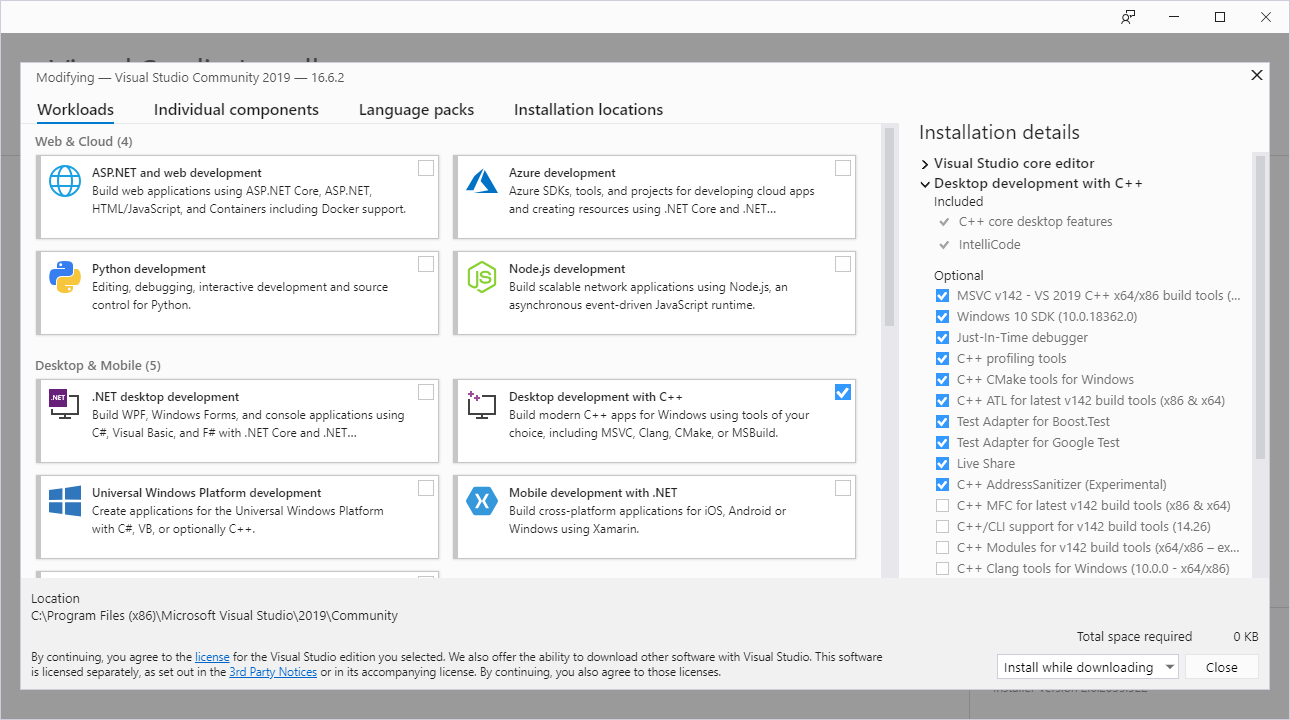
\includegraphics[width=\textwidth]{000installworkload}
\caption{Selecteren van de C++-workload.}
\label{fig:000installworkload}
\end{figure}


Start Visual Studio door op het icoon te klikken. Visual Studio opent een beginscherm waarin een nieuw project kan worden aangemaakt. Dit is te zien in figuur~\ref{fig:001newproject}. Klik op het kader \texttt{Create a new project}.

\begin{figure}[H]
\centering
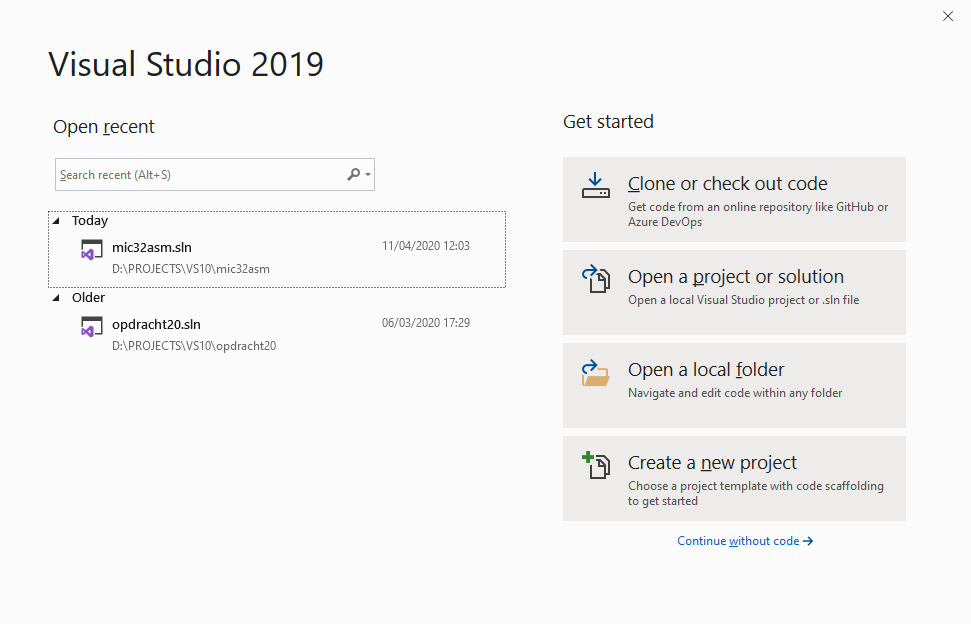
\includegraphics[scale=0.5]{001newproject}
\caption{Aanmaken van een nieuw project.}
\label{fig:001newproject}
\end{figure}

Er wordt een nieuw scherm geopend, zie figuur~\ref{fig:002create}. Klik daarin op het kader \texttt{Empty Project}. \textbf{Klik niet op\texttt{ Console App}.}

\begin{figure}[H]
\centering
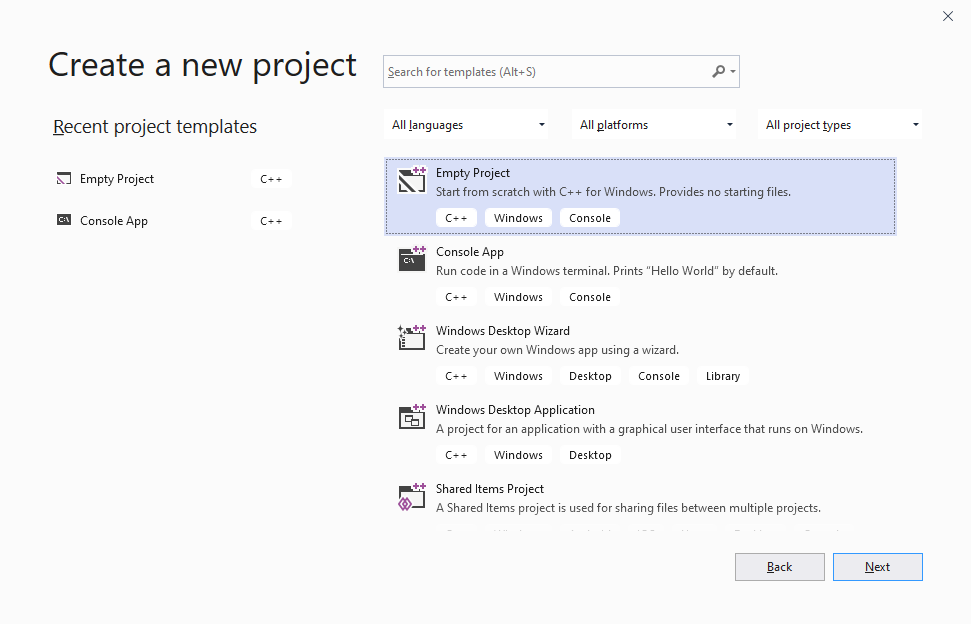
\includegraphics[scale=0.5]{002create}
\caption{Aanmaken van een leeg project.}
\label{fig:002create}
\end{figure}

Daarna moeten wat gegevens worden ingevuld. Vul de projectnaam in en de map waarin het project terecht moet komen. Vink de checkbox onderaan aan en klik op de knop \texttt{Create}. Zie figuur~\ref{fig:003configure}.

\begin{figure}[H]
\centering
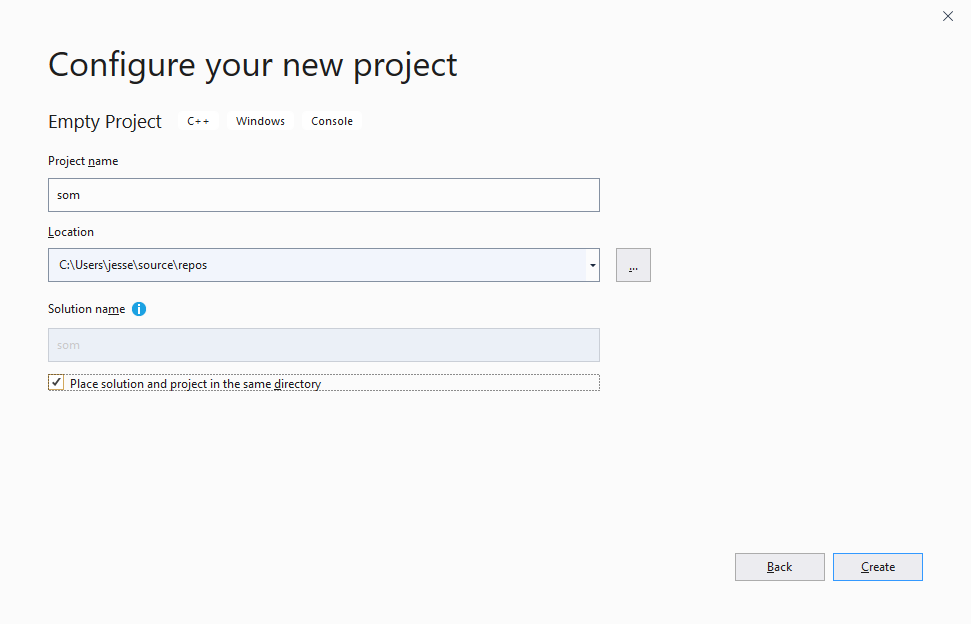
\includegraphics[scale=0.5]{003configure}
\caption{Gegevens van het project invoeren.}
\label{fig:003configure}
\end{figure}

Visual Studio komt nu met het hoofdscherm waarin een aantal vensters (Engels: pane) te zien zijn. Er is nog geen C-bestand aangemaakt, dat moeten we zelf doen. In de \textsl{Solution Explorer} aan de rechterkant is een map \texttt{Source Files} te zien. Ga met de muis-pointer daar op staan en klik op de \textbf{rechter} muisknop.

Selecteer daarna de optie \texttt{Add} en daarna \texttt{New item..}. Zie figuur~\ref{fig:004addnewitem}.

\begin{figure}[H]
\centering
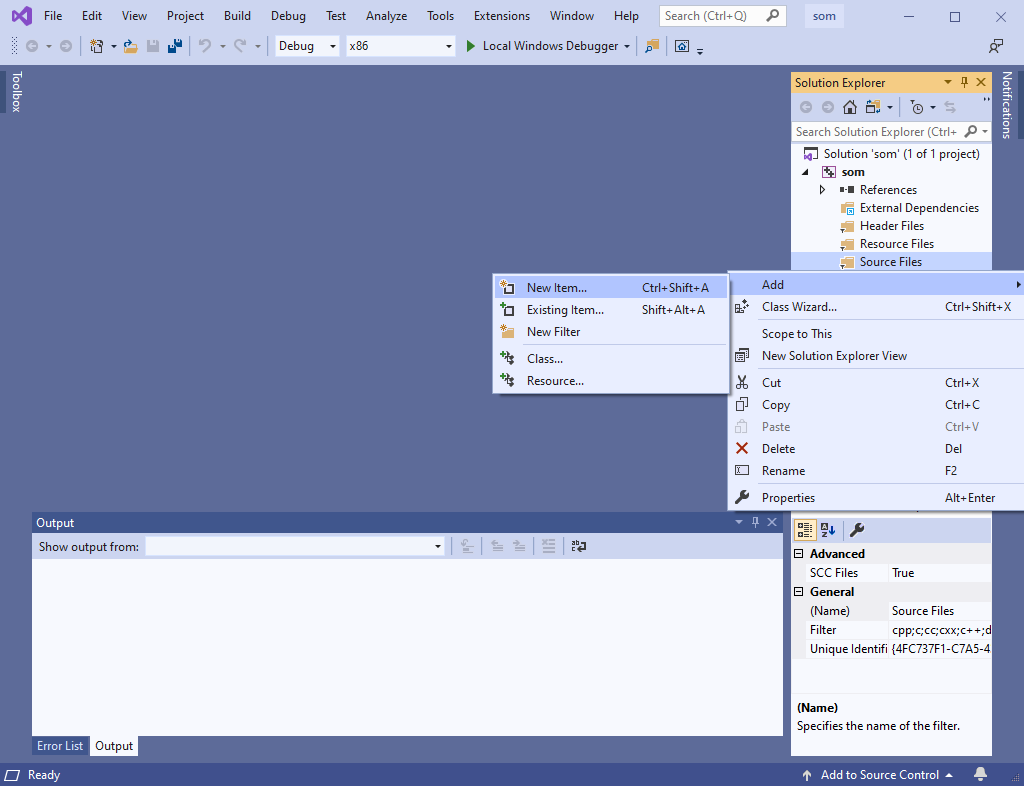
\includegraphics[scale=0.5]{004addnewitem}
\caption{Een nieuw bestand aanmaken.}
\label{fig:004addnewitem}
\end{figure}

In het volgende scherm moet een bestandstype en een naam worden opgegeven. Klik op \texttt{C++ File (.cpp)}. Vul onderin bij  \texttt{Name} de naam van het bestand in \textbf{en zorg ervoor dat de naam eindigt met \texttt{.c}}, anders wordt een C++-bestand aangemaakt. Klik daarna op de knop \texttt{Add}. Zie figuur~\ref{fig:005enterfilename}.

Voer het programma in zoals te zien is in figuur~\ref{fig:006build}. Klik daarna op de knop \texttt{Local Windows Debugger}. Het programma wordt nu gecompileerd en als er geen fouten zijn gevonden, wordt het programma uitgevoerd. Herstel eventuele fouten die door de compiler gevonden worden en herstart de compilatie.

Het programma drukt de regel \texttt{De som van 3 en 7 is 10} af. Dit wordt gedaan in een zogenoemde \textsl{console}. Dit is te zien in figuur~\ref{fig:007output}.

De tutorial is hiermee ten einde.

\begin{figure}[H]
\centering
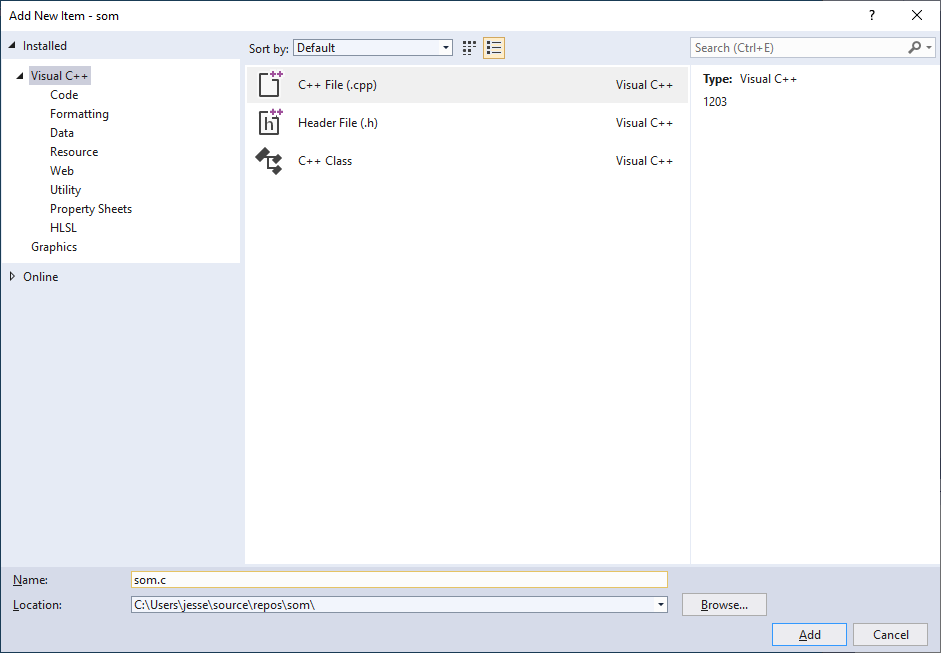
\includegraphics[scale=0.5]{005enterfilename}
\caption{Gegevens van het C-bestand invullen.}
\label{fig:005enterfilename}
\end{figure}

\begin{figure}[H]
\centering
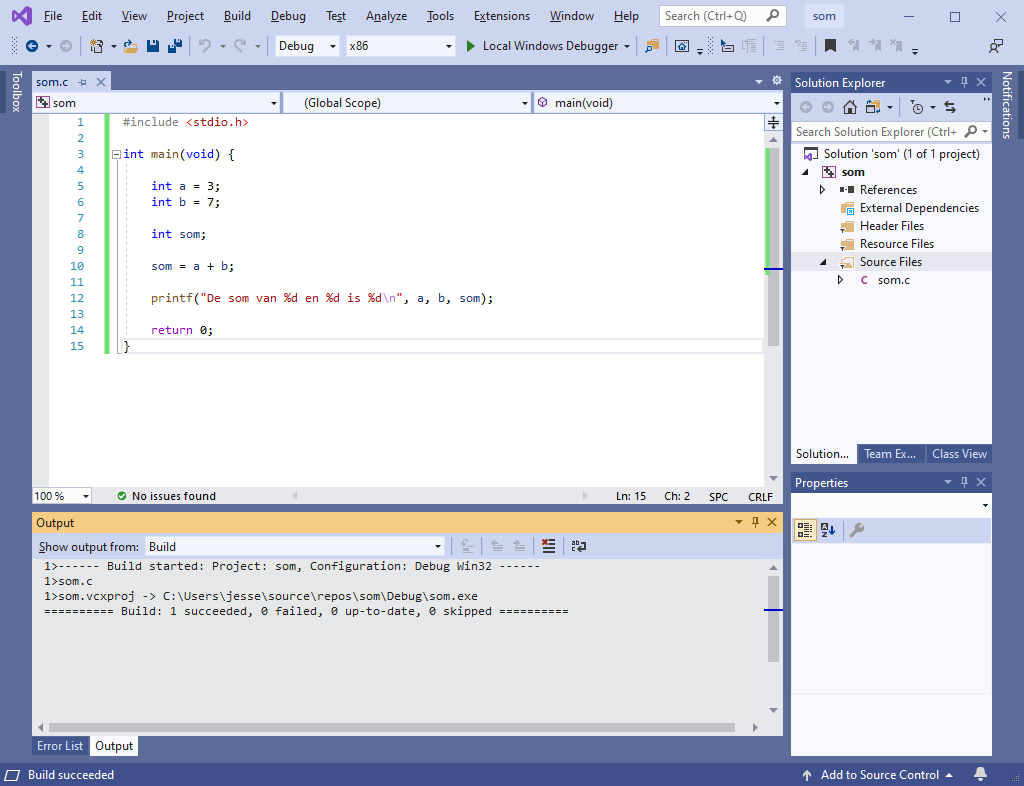
\includegraphics[scale=0.5]{006build}
\caption{Compileren en starten van de executable.}
\label{fig:006build}
\end{figure}

\begin{figure}[H]
\centering
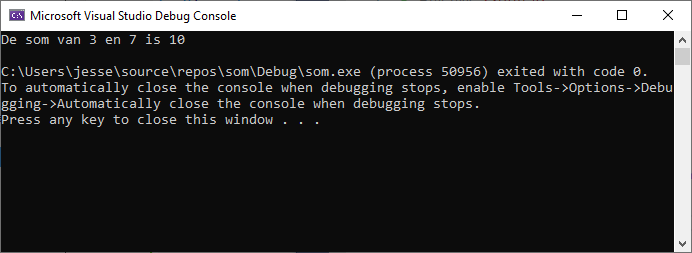
\includegraphics[scale=0.5]{007output}
\caption{Uitvoer van het programma in een console.}
\label{fig:007output}
\end{figure}



\section{Installatie Code::Blocks}
\label{sec:installcodeblocks}

In deze bijlage zijn instructies te vinden voor het installeren en gebruiken van Code::Blocks 20.03. De instructies zijn als volgt:

\begin{itemize}
\item Download Code::Blocks van \url{https://sourceforge.net/projects/codeblocks/files/Binaries/20.03/Windows/codeblocks-20.03mingw-setup.exe/download} (let erop dat in de naam de term \texttt{mingw} staat)
\item Installeer vervolgens Code::Blocks door de gedownloade executable te runnen. (Bij installatie continu op \texttt{next} drukken)
\item Bij het opstarten van Code::Blocks wordt er gevraagd naar de compiler die gebruikt zal gaan worden. Als het goed is, is er al \'e\'en geselecteerd en hoef je alleen op \texttt{OK} te drukken.
\item Nu kun je een project aanmaken en code gaan compileren en runnen:
\begin{enumerate}[label=\alph*.]
\item \lstinline[language=,literate=]|File->New->Project|
\item Selecteer \lstinline[language=,literate=]|Console application| + \lstinline|GO|
\item \lstinline[language=,literate=]|Next|
\item Selecteer \lstinline[language=,literate=]|C| (!!!NIET!!! \lstinline[language=,literate=]|C++|)
\item \lstinline[language=,literate=]|Project Title = helloworld|
\item \lstinline[language=,literate=]|Folder to create project in|: Selecteer een map die je later nog terug kan vinden\ldots
\item \lstinline[language=,literate=]|Next|
\item \lstinline[language=,literate=]|Finish| (vinkjes aan, GNU GCC compiler geselecteerd)
\item Links in de projectomgeving is nu de file \lstinline[language=,literate=]|main.c| te vinden met code:

\begin{lstlisting}
#include <stdio.h>
#include <stdlib.h>

int main(void)
{
    printf("Hello world\n");
    return 0;
}
\end{lstlisting}
\item Klik op \lstinline|Build| (Ctrl+F9) (het tandwiel symbool bovenaan)
\item Klik op \lstinline|Run| (Ctrl+F10) (het groene play symbool bovenaan)
\end{enumerate}
\end{itemize}


\iffalse
\section{Moeilijkheidsgraad}
In de onderstaande tabel is de moeilijkheidsgraad te vinden. A = eenvoudig, B = iets moeilijker, C = lastig, D = moeilijk, E = heel moeilijk.
 
\begin{multicols}{4}
2.2 B\\
2.3 A\\
2.4 A\\
2.5 C\\
2.6 A\\
2.7 A\\
2.8 B\\
2.9 D\\
2.10 D\\
2.11 D\\
2.12 B\\
2.13 C\\
2.14 C\\
2.15 D
\end{multicols}

\begin{multicols}{4}
3.2 A\\
3.3 A\\
3.4 A\\
3.5 B\\
3.6 B\\
3.7 D\\
3.8 C\\
3.9 A\\
3.10 B\\
3.11 B\\
3.12 A\\
3.13 D
\end{multicols}

\begin{multicols}{4}
4.2 B\\
4.3 B\\
4.4 A\\
4.5 B\\
4.6 A\\
4.7 A\\
4.8 A\\
4.9 B\\
4.10 C\\
4.11 C\\
4.12 C\\
4.13 B\\
4.14 C
\end{multicols}

\begin{multicols}{4}
5.2 A\\
5.3 A\\
5.4 B\\
5.5 C\\
5.6 A\\
5.7 C\\
5.8 D\\
5.9 A\\
5.10 B\\
5.11 D\\
5.12 B\\
5.13 D\\
5.14 D\\
5.15 C\\
5.16 B\\
5.17 C\\
5.18 D\\
5.19 E\\
5.20 D\\
\end{multicols}

\begin{multicols}{4}
6.2 A\\
6.3 C\\
6.4 D\\
6.5 C\\
6.6 B\\
6.7 C\\
6.8 D\\
6.9 C\\
6.10 B\\
6.11 A\\
6.12 D
\end{multicols}
\fi
\end{document}
